\documentclass[10pt]{beamer}

\usetheme{metropolis}
\usepackage{appendixnumberbeamer}

\usepackage[]{algorithm2e}
% \usepackage{algorithm}
% \usepackage{algpseudocode}
\usepackage{amsfonts}
\usepackage[ngerman]{babel}
\usepackage[backend=biber]{biblatex}
\usepackage{booktabs}
\usepackage[scale=2]{ccicons}
\usepackage{graphicx}
\usepackage{hyperref}
\usepackage[utf8]{inputenc} 
\usepackage{lipsum}
\usepackage{listings}
\usepackage{multirow}

\usepackage{pgfplots}
\usepackage{xcolor}

\addbibresource{presentation.bib}

\SetInd{0.25em}{0.4em}


\usepgfplotslibrary{dateplot}

\usepackage{xspace}
\newcommand{\themename}{\textbf{\textsc{metropolis}}\xspace}

\addto{\captionsngerman}{%
  \renewcommand*{\figurename}{Abb.}
}

\let\svthefootnote\thefootnote

\definecolor{mGreen}{rgb}{0,0.6,0}
\definecolor{mGray}{rgb}{0.5,0.5,0.5}
\definecolor{mPurple}{rgb}{0.58,0,0.82}

\lstdefinestyle{CStyle}{
    commentstyle=\color{mGreen},
    keywordstyle=\color{magenta},
    numberstyle=\tiny\color{mGray},
    stringstyle=\color{mPurple},
    basicstyle=\footnotesize,
    breakatwhitespace=false,
    breaklines=true,
    captionpos=b,
    keepspaces=true,
    numbers=left,
    numbersep=5pt,
    showspaces=false,
    showstringspaces=false,
    showtabs=false,
    tabsize=2,
    language=C
}

\title{Ein skalierbarer L\"oser f\"ur Randwertprobleme unter Verwendung der
       Greenschen Kreuzapproximationsmethode und GPUs}
\date{\today}
\author{Bennet Carstensen}
\institute{Christian-Albrechts-Universität zu Kiel\\
           Institut für Informatik\\
           Scientific Computing}
% \titlegraphic{\hfill\includegraphics[height=1.5cm]{logo.pdf}}

\begin{document}

\maketitle

\begin{frame}{Agenda}
  \setbeamertemplate{section in toc}[sections numbered]
  \tableofcontents[hideallsubsections]
\end{frame}

\section{Einleitung}

\begin{frame}{Randwertprobleme}
  \begin{columns}
    \column{0.675\linewidth}
      \begin{itemize}
        \visible<1->{\item Wird verwendet in der
                     \begin{itemize}
                       \item Elektrostatik
                       \item Wärmeleitung
                       \item Akustik
                     \end{itemize}}
        \item \visible<1->{Sei \(\Omega \subseteq \mathbb{R}^{d}\) gegeben,
                           \( d \in \{ 2, 3 \} \)}
        \item \visible<2->{\( \int\limits_{\Omega} g(x, y) u(y) dy = f(x)
                              \newline \text{ für alle } x \in \Omega \)}
        \item \visible<2->{z.B. \(g(x, y) = \frac{1}{4\pi\left\lVert x - y
                           \right\rVert_{2}}\) (Fundamentallösung der
                           Laplacegleichung)}
      \end{itemize}
    \column{0.325\linewidth}
      \centering
      \begin{overprint}
        \onslide<1>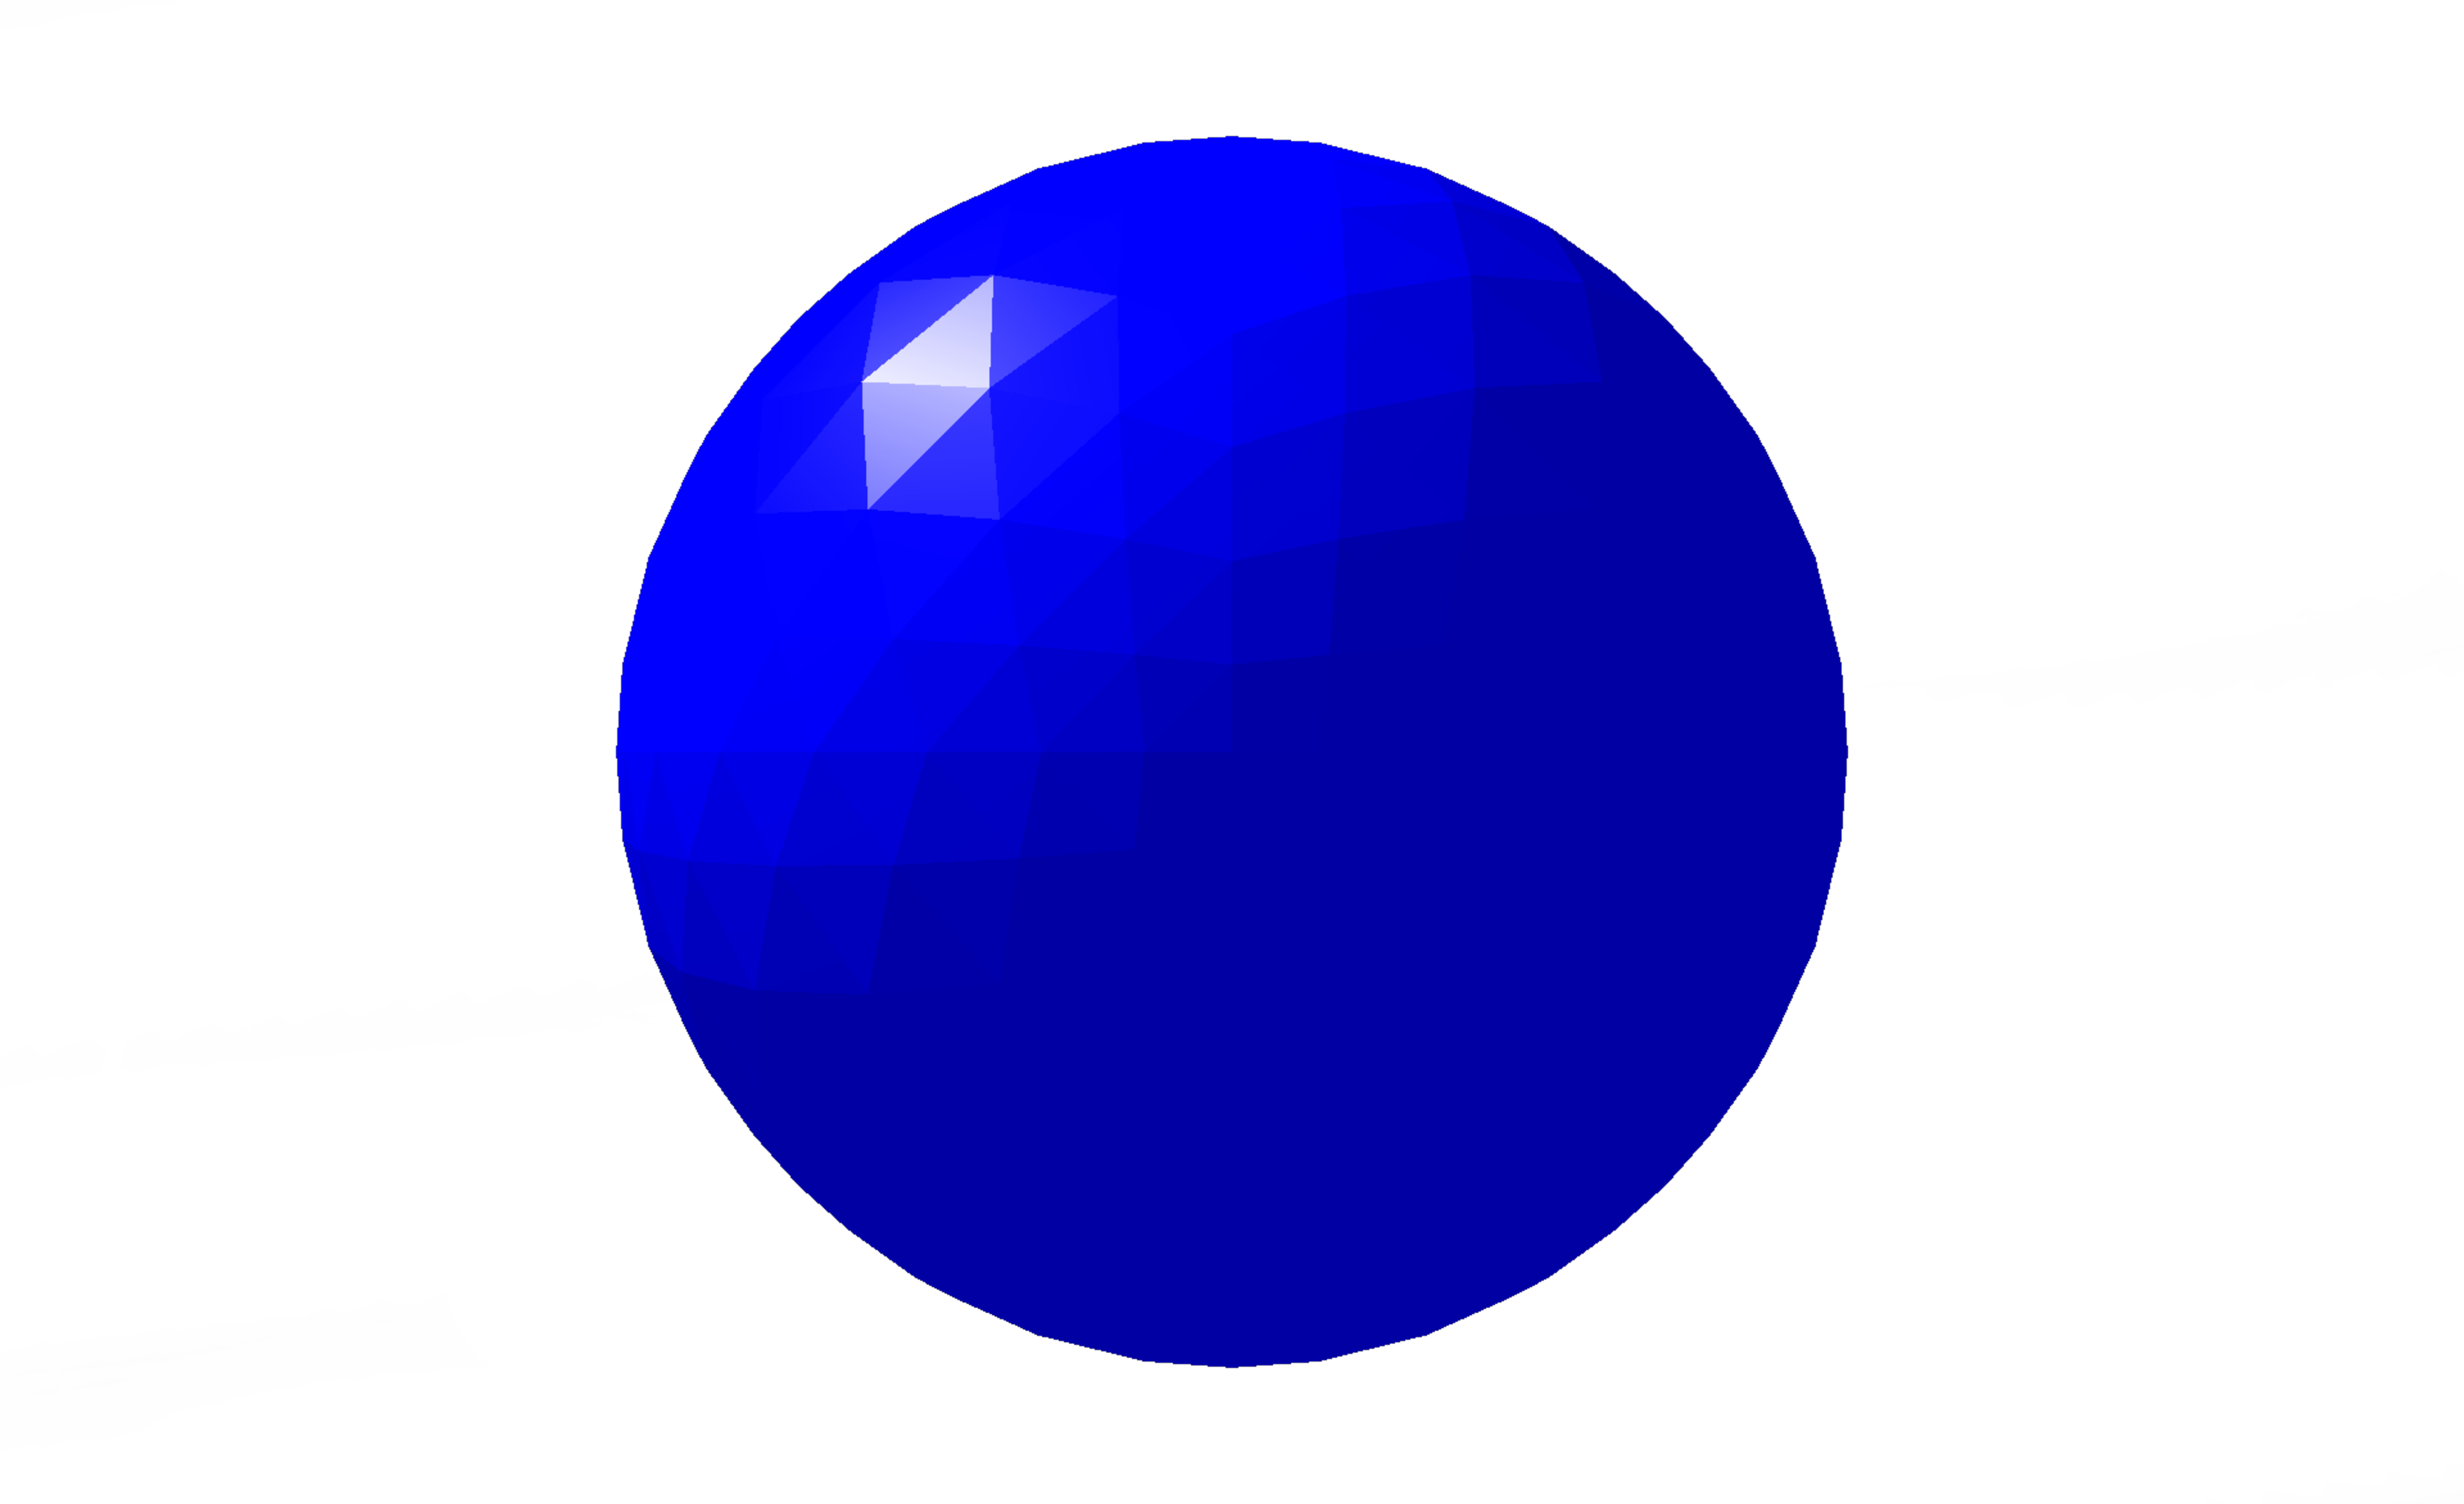
\includegraphics[width=1.5\linewidth]{figures/fg-sphere-full.pdf}
        \onslide<2>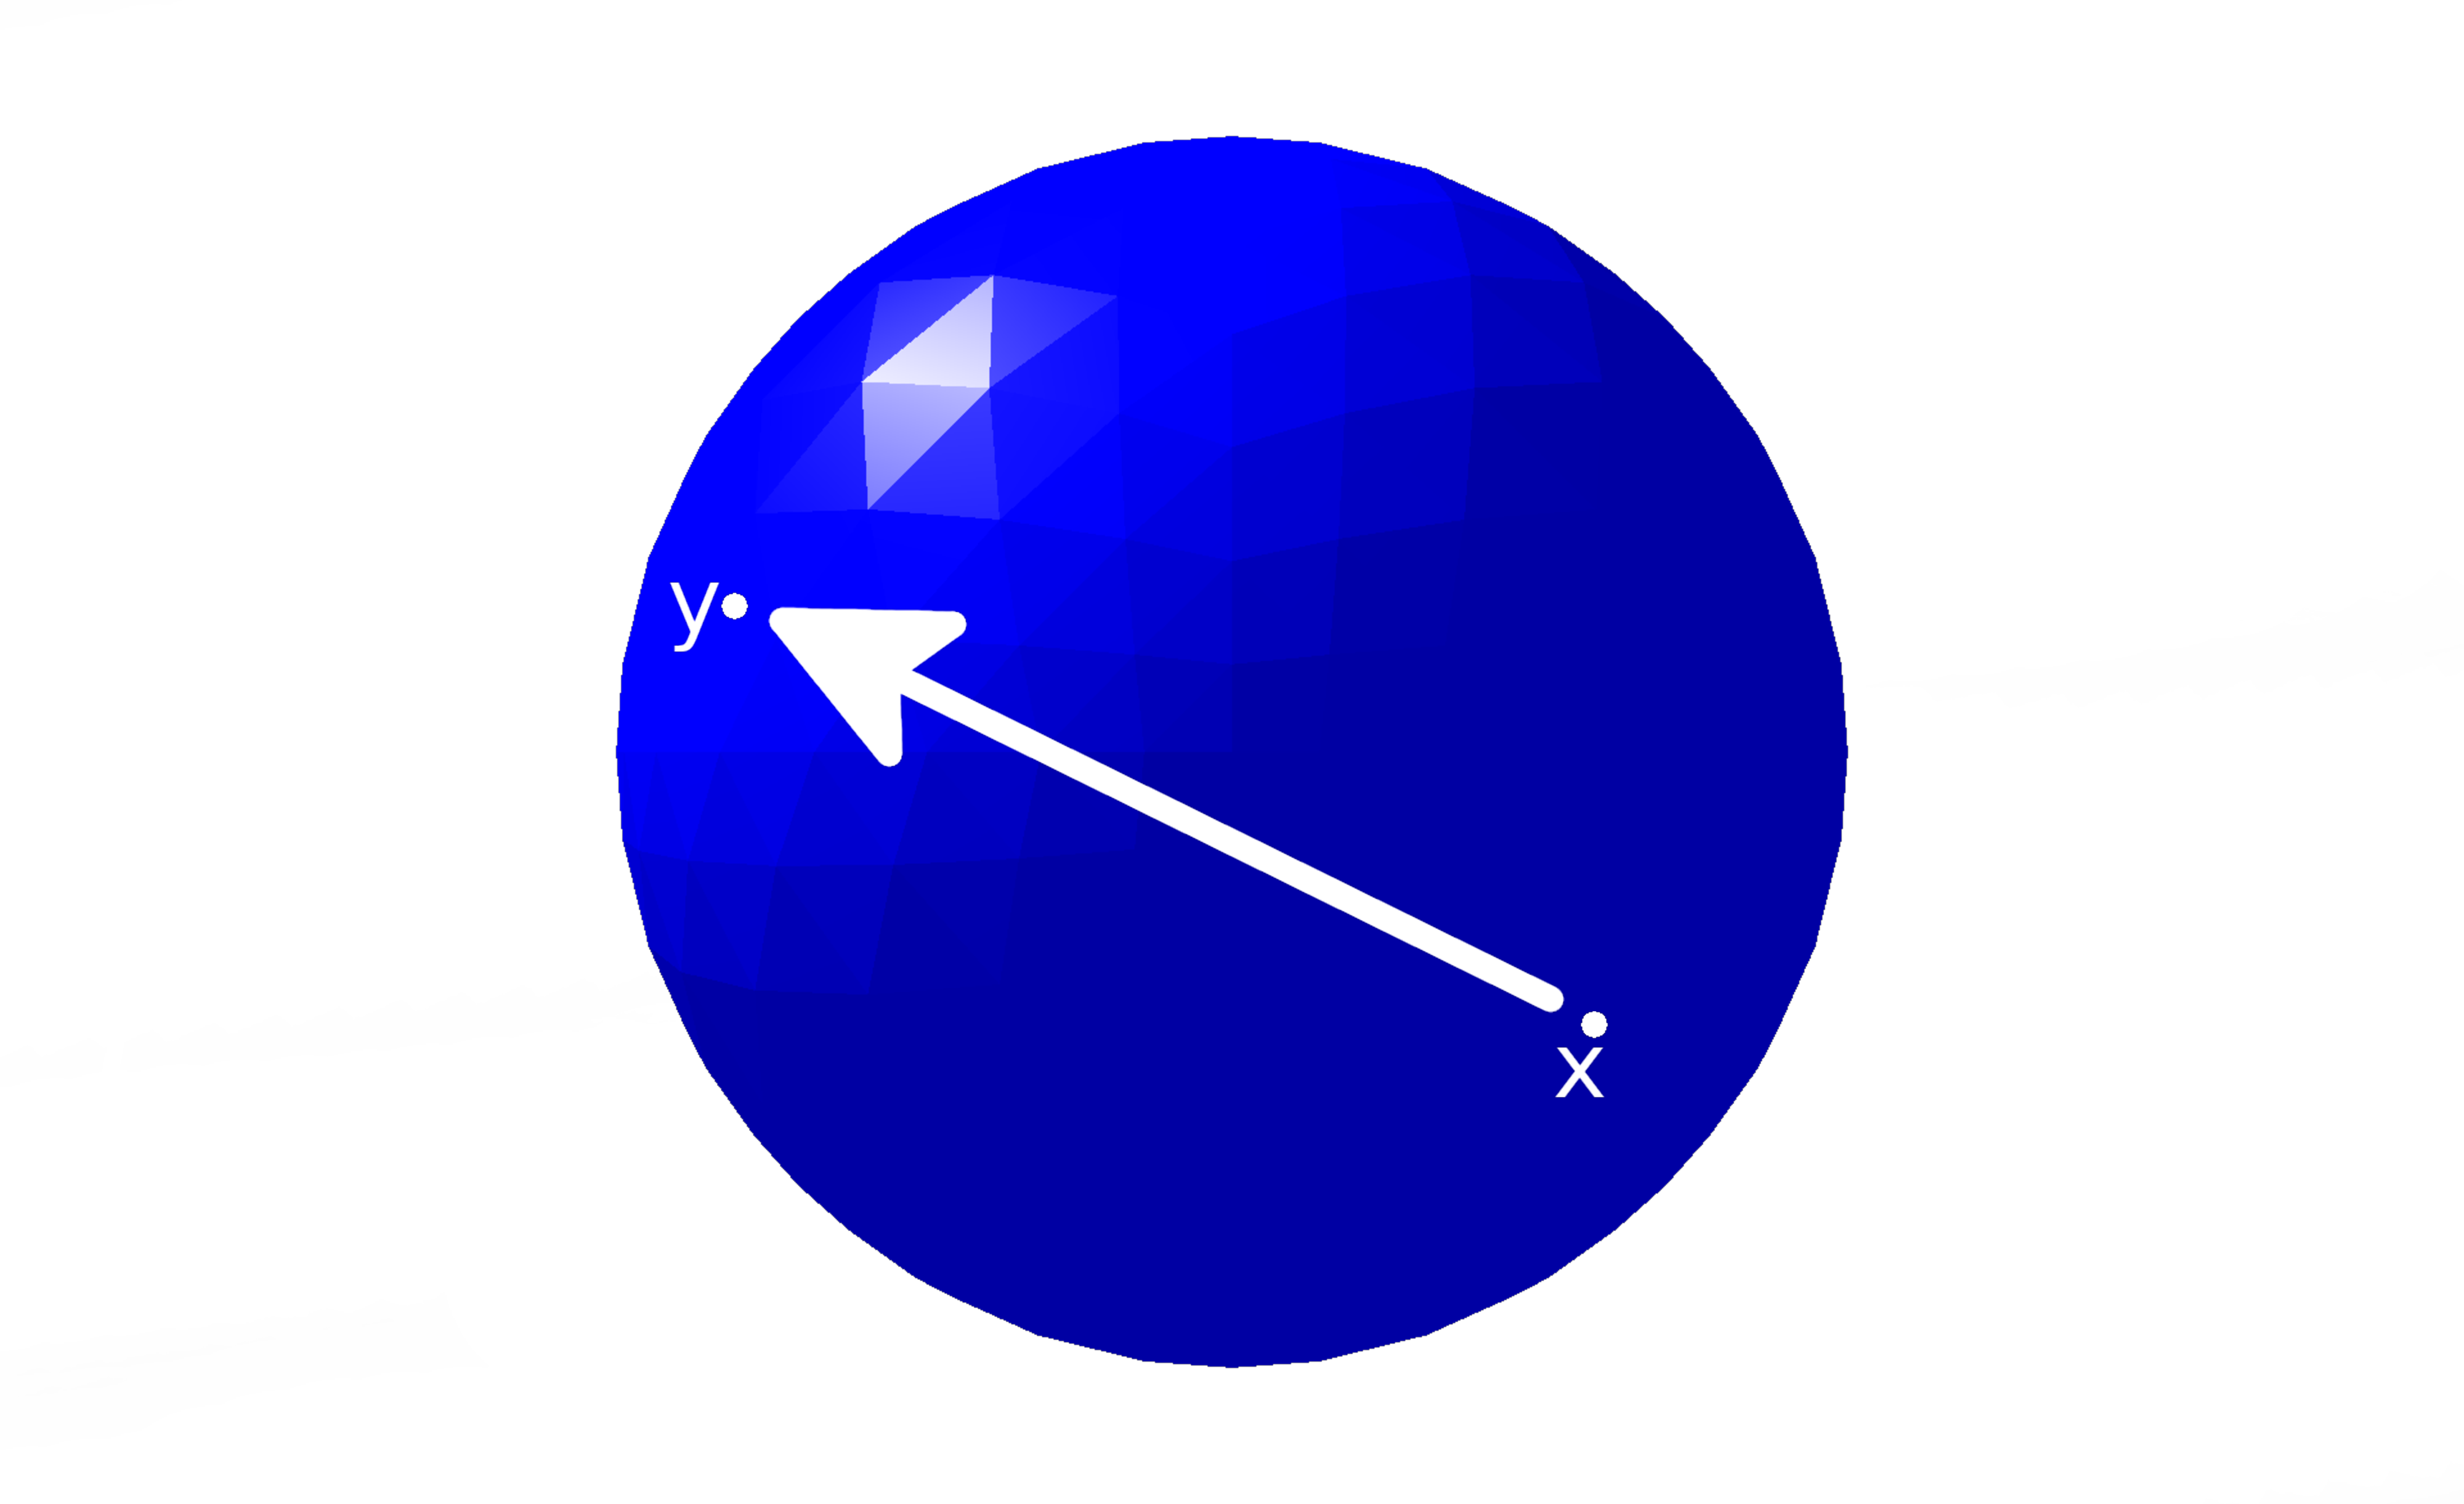
\includegraphics[width=1.5\linewidth]{figures/fg-sphere-full-inf.pdf}
      \end{overprint}

  \end{columns}
  \footnotesize
  \let\thefootnote\relax\footnote{Steffen Börm und Sven Christophersen.
  \href{https://link.springer.com/article/10.1007\%2Fs00211-015-0757-y}{
  ``Approximation of integral operators by Green quadrature and nested cross 
  approximation''}. In:   \textit{Numerische Mathematik} 133.3 (2016), S. 
  409-442, 2016.}
  \addtocounter{footnote}{-1}\let\thefootnote\svthefootnote\relax
  \normalsize
\end{frame}

\begin{frame}{Diskretisierung}
  \begin{columns}
    \column{0.675\linewidth}
      Galerkin-Diskretisierung mit Basisfunktionen\\
      \({(\varphi_{i})}_{i = 1}^{n} \text{ und }
        {(\psi_{j})}_{j = 1}^{n}, n \in \mathbb{N}\)
      \begin{itemize}
        \item \( V_{n} = span\{ \varphi_{i} : i \in \{ 1, \hdots, n\} \},
                \newline
                U_{n} = span\{ \psi_{j} : j \in \{ 1, \hdots, n\} \} \)
        \item Finde \(u_{n} \in U_{n}\) mit\\
        \small{\( \int\limits_{\Omega} v_{n}(x) \int\limits_{\Omega} g(x,y) \
                  u_{n}(y)
                   \ dy \ dx = \int\limits_{\Omega} v_{n}(x) \ f(x) \ dx \) \\
                für alle \(v_{n} \in V_{n}\)}
      \end{itemize}
    \column{0.325\linewidth}
      \centering
      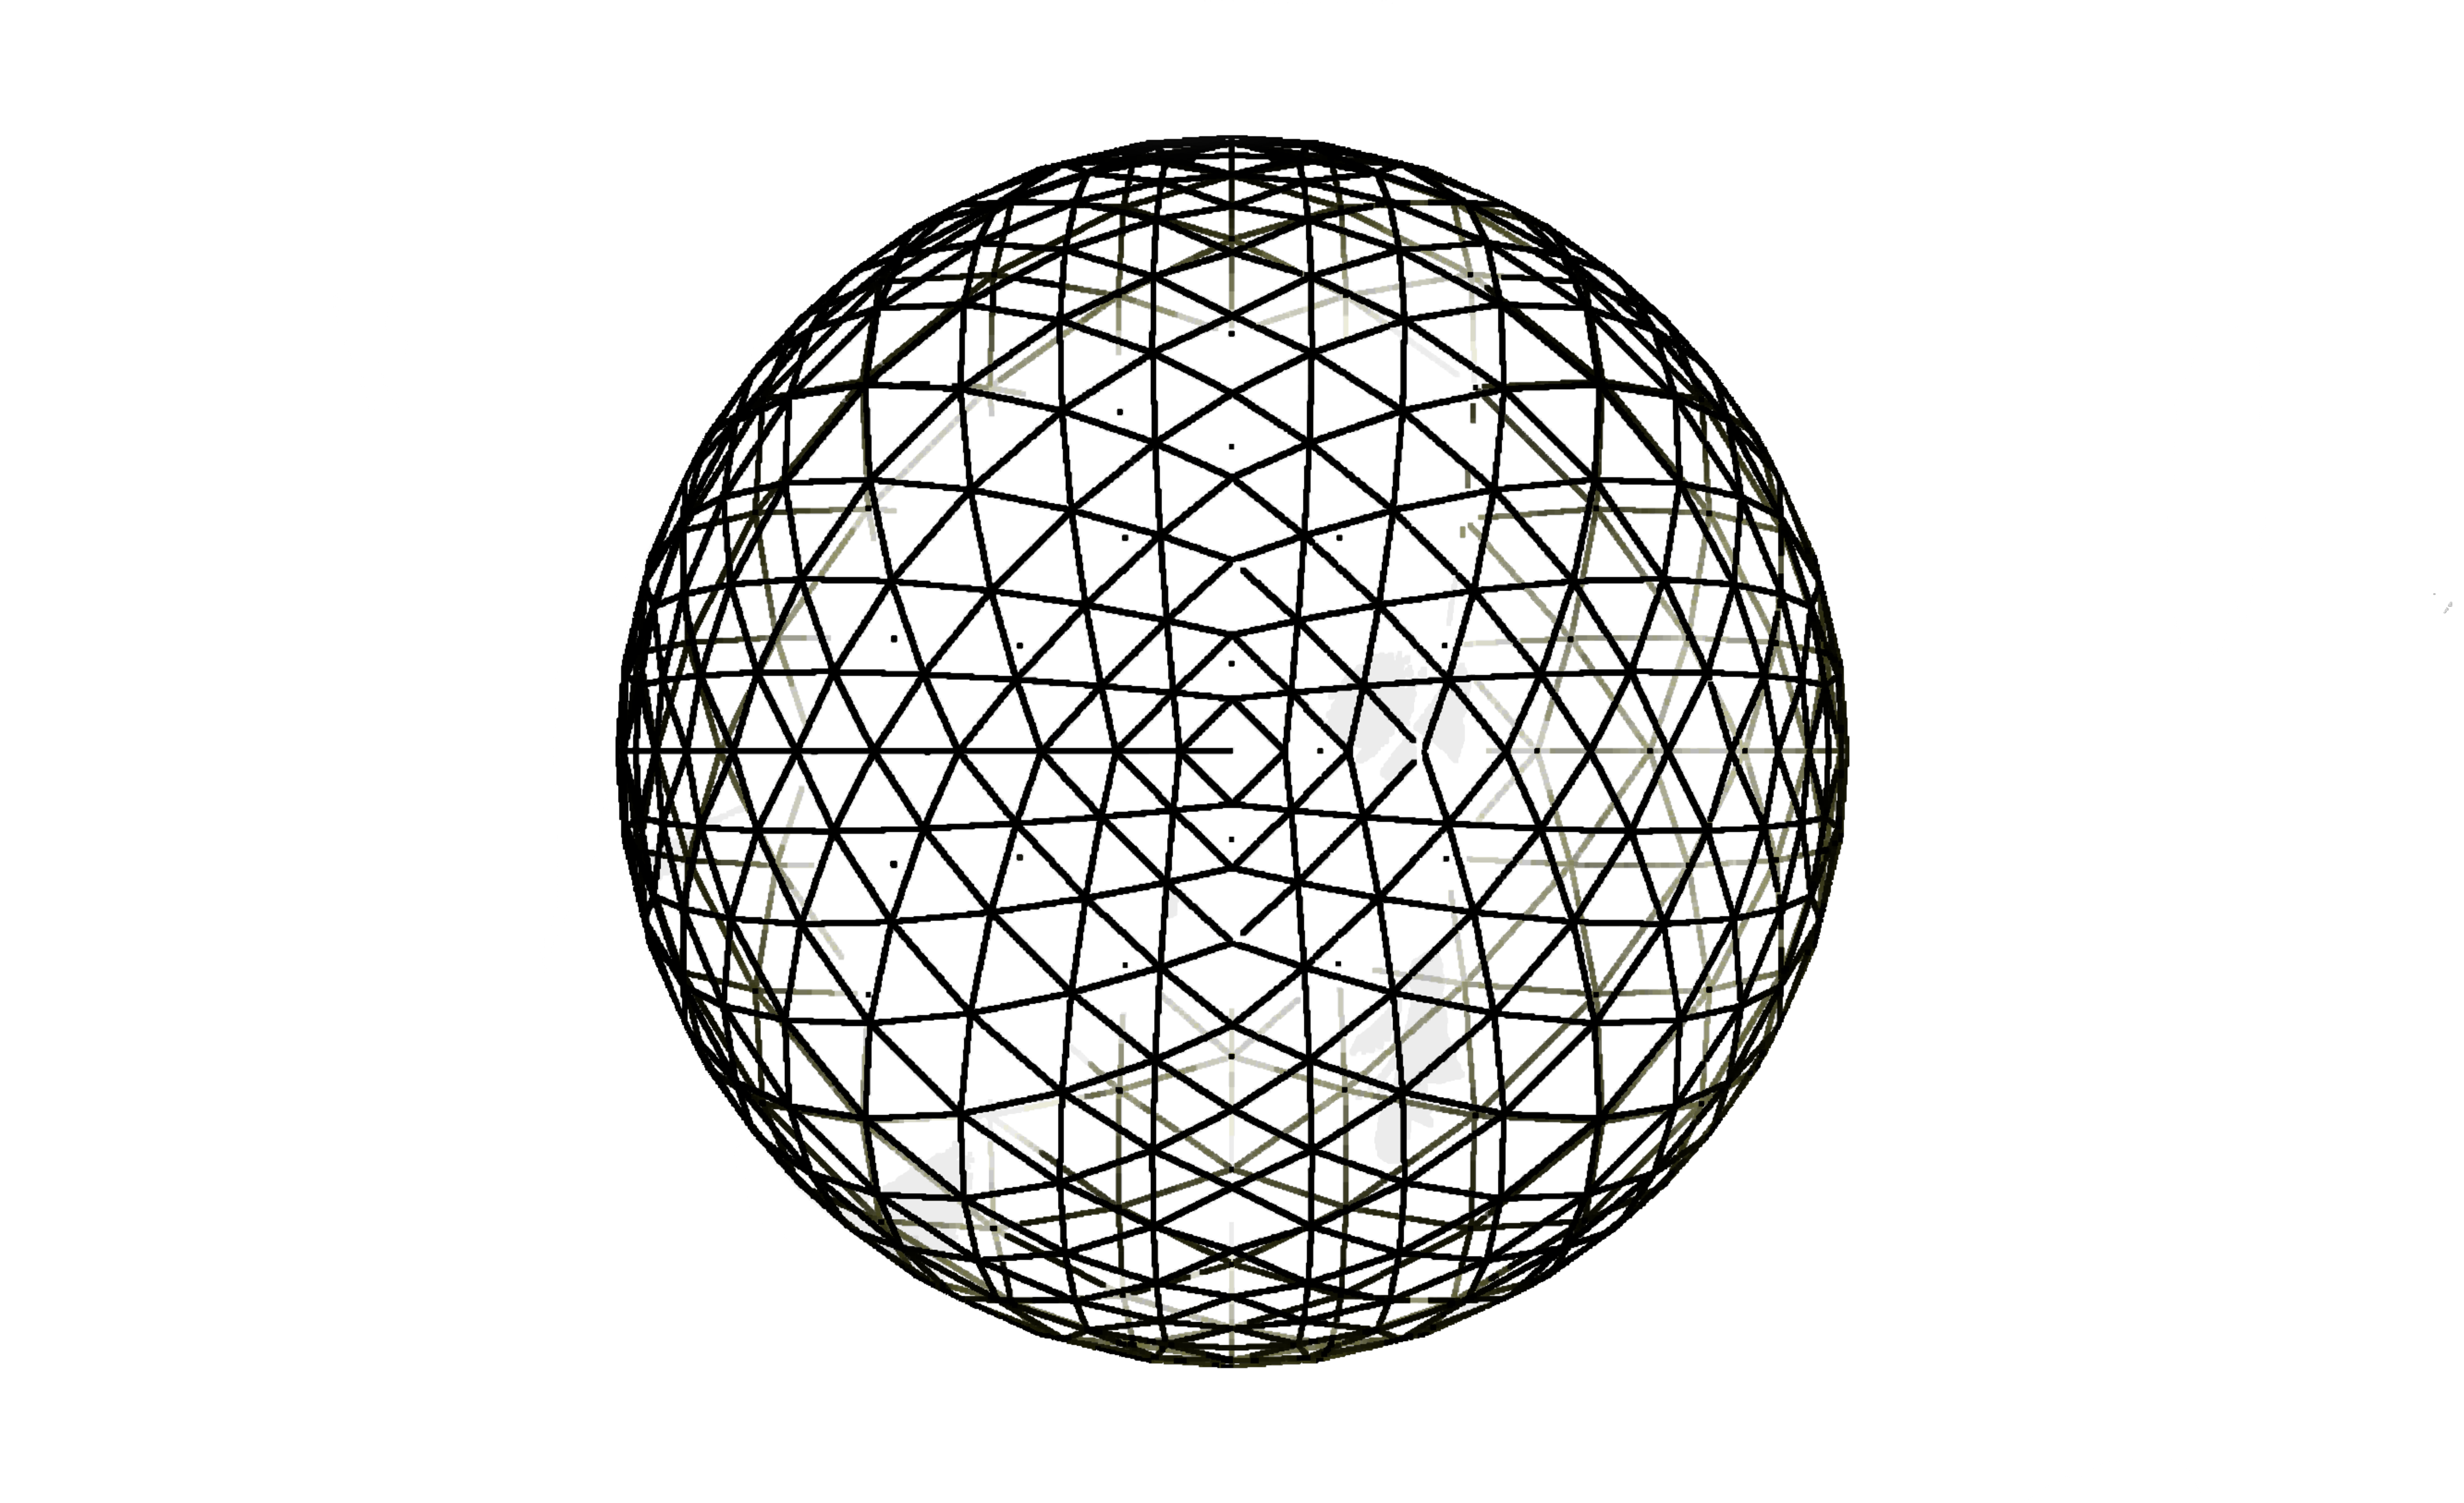
\includegraphics[width=1.5\linewidth]{figures/fg-sphere-tri.pdf}
  \end{columns}
  \footnotesize
  \let\thefootnote\relax\footnote{Steffen Börm und Sven Christophersen.
  \href{https://link.springer.com/article/10.1007\%2Fs00211-015-0757-y}{
  ``Approximation of integral operators by Green quadrature and nested cross 
  approximation''}. In:   \textit{Numerische Mathematik} 133.3 (2016), S. 
  409-442, 2016.}
  \addtocounter{footnote}{-1}\let\thefootnote\svthefootnote\relax
  \normalsize
\end{frame}

\begin{frame}{Lineares Gleichungssystem}
  Sei \(u_{n}  = \sum\limits_{j = 1}^{n} \psi_{j} z_{j}, z_{j} \in
        \mathbb{R} \)
  \begin{itemize}
    \item Finde \(z = (z_{1}, \hdots, z_{n}) \in \mathbb{R}^{n}\) mit\\
          \(Gz = b\)
    \item \(g_{ij} = \int\limits_{\Omega} \varphi_{i}(x) \int\limits_{\Omega}
            g(x, y) \ \psi_{j}(y) \ dy \ dx\)
    \item \(b_{i} = \int\limits_{\Omega} \varphi_{i} \ f(x) \ dx\)
    \item \(i, j \in \{ 1, \hdots, n \}\)
  \end{itemize}
  \footnotesize
  \let\thefootnote\relax\footnote{Steffen Börm und Sven Christophersen.
  \href{https://link.springer.com/article/10.1007\%2Fs00211-015-0757-y}{
  ``Approximation of integral operators by Green quadrature and nested cross 
  approximation''}. In:   \textit{Numerische Mathematik} 133.3 (2016), S. 
  409-442, 2016.}
  \addtocounter{footnote}{-1}\let\thefootnote\svthefootnote\relax
  \normalsize
\end{frame}

\begin{frame}{Probleme \& Lösungsansätze}
  \begin{overprint}
    \onslide<1-2>
      \begin{table}[h]
        \begin{tabular}{rrr} \toprule
          \multirow{2}{*}{Dimension} & \multicolumn{2}{c}{Speicherbedarf (in 
          GB)} \\ \cmidrule{2-3}
                      & Galerkin & \\ \midrule
              16\,384 &      1.0 & \\
              32\,768 &      4.0 & \\
              65\,536 &     16.0 & \\
             131\,072 &     64.0 & \\
             262\,144 &    256.0 & \\ \bottomrule
        \end{tabular}
      \end{table}
    \onslide<3>
      \begin{table}[h]
        \begin{tabular}{rrr} \toprule
          \multirow{2}{*}{Dimension} & \multicolumn{2}{c}{Speicherbedarf (in 
          GB)} \\ \cmidrule{2-3}
                      & Galerkin & \(\mathcal{H}^2\)-Matrix \\ \midrule
              16\,384 &      1.0 & 0.206 \\
              32\,768 &      4.0 & 0.438 \\
              65\,536 &     16.0 & 0.883 \\
             131\,072 &     64.0 & 1.809 \\
             262\,144 &    256.0 & 3.571 \\ \bottomrule
        \end{tabular}
      \end{table}
  \end{overprint}

  \begin{itemize}
    \item \visible<1->{Problem: \(G\) meist vollbesetzt \(\Rightarrow\) hohe
                       Speicheranforderungen und hoher Rechenaufwand}
    \visible<2->{\item Lösungsansätze:}
    \begin{itemize}
      \item \visible<2->{Schnelle Multipol-Methode (bessere
                         Laufzeitkomplexität)}
      \item \visible<3->{\(\mathcal{H}^2\)-Matrizen +
                           Greensche Kreuzapproximationsmethode\\
                           (engl. \textit{Green cross approximation (GCA)
                           method})\\
                           (geringere Speicheranforderungen \(\Rightarrow\)
                           bessere Laufzeitkomplexität)}
    \end{itemize}
  \end{itemize}
\end{frame}

\begin{frame}{Problem \& Lösungsansätze}
  \begin{figure}
    \centering
    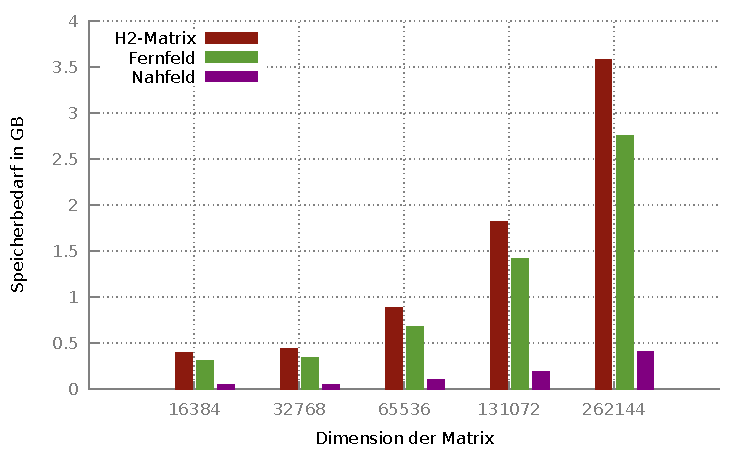
\includegraphics[width=.45\linewidth]{figures/fg-memory-h2-nf-ff.pdf}
    \caption{Speicherbedarf einer \(\mathcal{H}^2\)-Matrix und deren Blockmatrizen}
  \end{figure}
  \begin{itemize}
    \item Problem: Reale Problemstellungen benötigen immer größere Matrizen
          \(\Rightarrow\) reduzierte Speicheranforderungen durch
          \(\mathcal{H}^2\)-Matrizen haben ihre Grenzen
    \item Lösungsansätz:
    \begin{itemize}
      \item Mehr Arbeitsspeicher
      \item Berechne reproduzierbare Untermatrizen einer
            \(\mathcal{H}^2\)-Matrix on-the-fly, wenn sie benötigt werden.
            (75-90 \% des Speicherbedarfs wird eingespart)
    \end{itemize}
  \end{itemize}
\end{frame}

\begin{frame}{Problem \& Lösungsansätze}
  \small
  \begin{table}[h]
    \begin{tabular}{rrr} \toprule
      \multirow{2}{*}{Dimension} & \multicolumn{2}{c}{Rechenzeit in
      ms\footnotemark[1]} \\ \cmidrule{2-3}
                & \(\mathcal{H}^2\)-MVM &
      \begin{tabular}{@{}c@{}}\(\mathcal{H}^2\)-MVM + \\ Blockmatrizen \\ on-the-fly\end{tabular} \\ \midrule
        16\,384 &    140 &  6\,980 \\
        32\,768 &    300 & 14\,640 \\
        65\,536 &    660 & 29\,440 \\
       131\,072 & 1\,190 & 60\,920 \\ \bottomrule
    \end{tabular}
  \end{table}
  \normalsize
  \begin{itemize}
    \item Problem: Wesentlich größerer Rechenaufwand bei letzterem Ansatz
    \item Lösungsansatz (diese Masterarbeit):
    \begin{itemize}
      \item Quadratur zur Auswertung der Integrale bestimmt Performance
      \item Quadratur ist äußerst parallelisierbar/vektorisierbar
      \item Auslagern der Auswertungen auf eine Grafikkarte
    \end{itemize}
  \end{itemize}
  \footnotesize
  \footnotetext[1]{Gleikommazahlen einfacher Genauigkeit auf einer Intel Xeon
                   E5-4640 mit OpenMP parallelisiert und AVX beschleunigt.}
  \normalsize
\end{frame}

\section{\(\mathcal{H}^2\)-Matrizen}

\begin{frame}{\(\mathcal{H}^2\)-Matrizen}
  \begin{figure}
    \begin{overprint}
      \onslide<1>\centering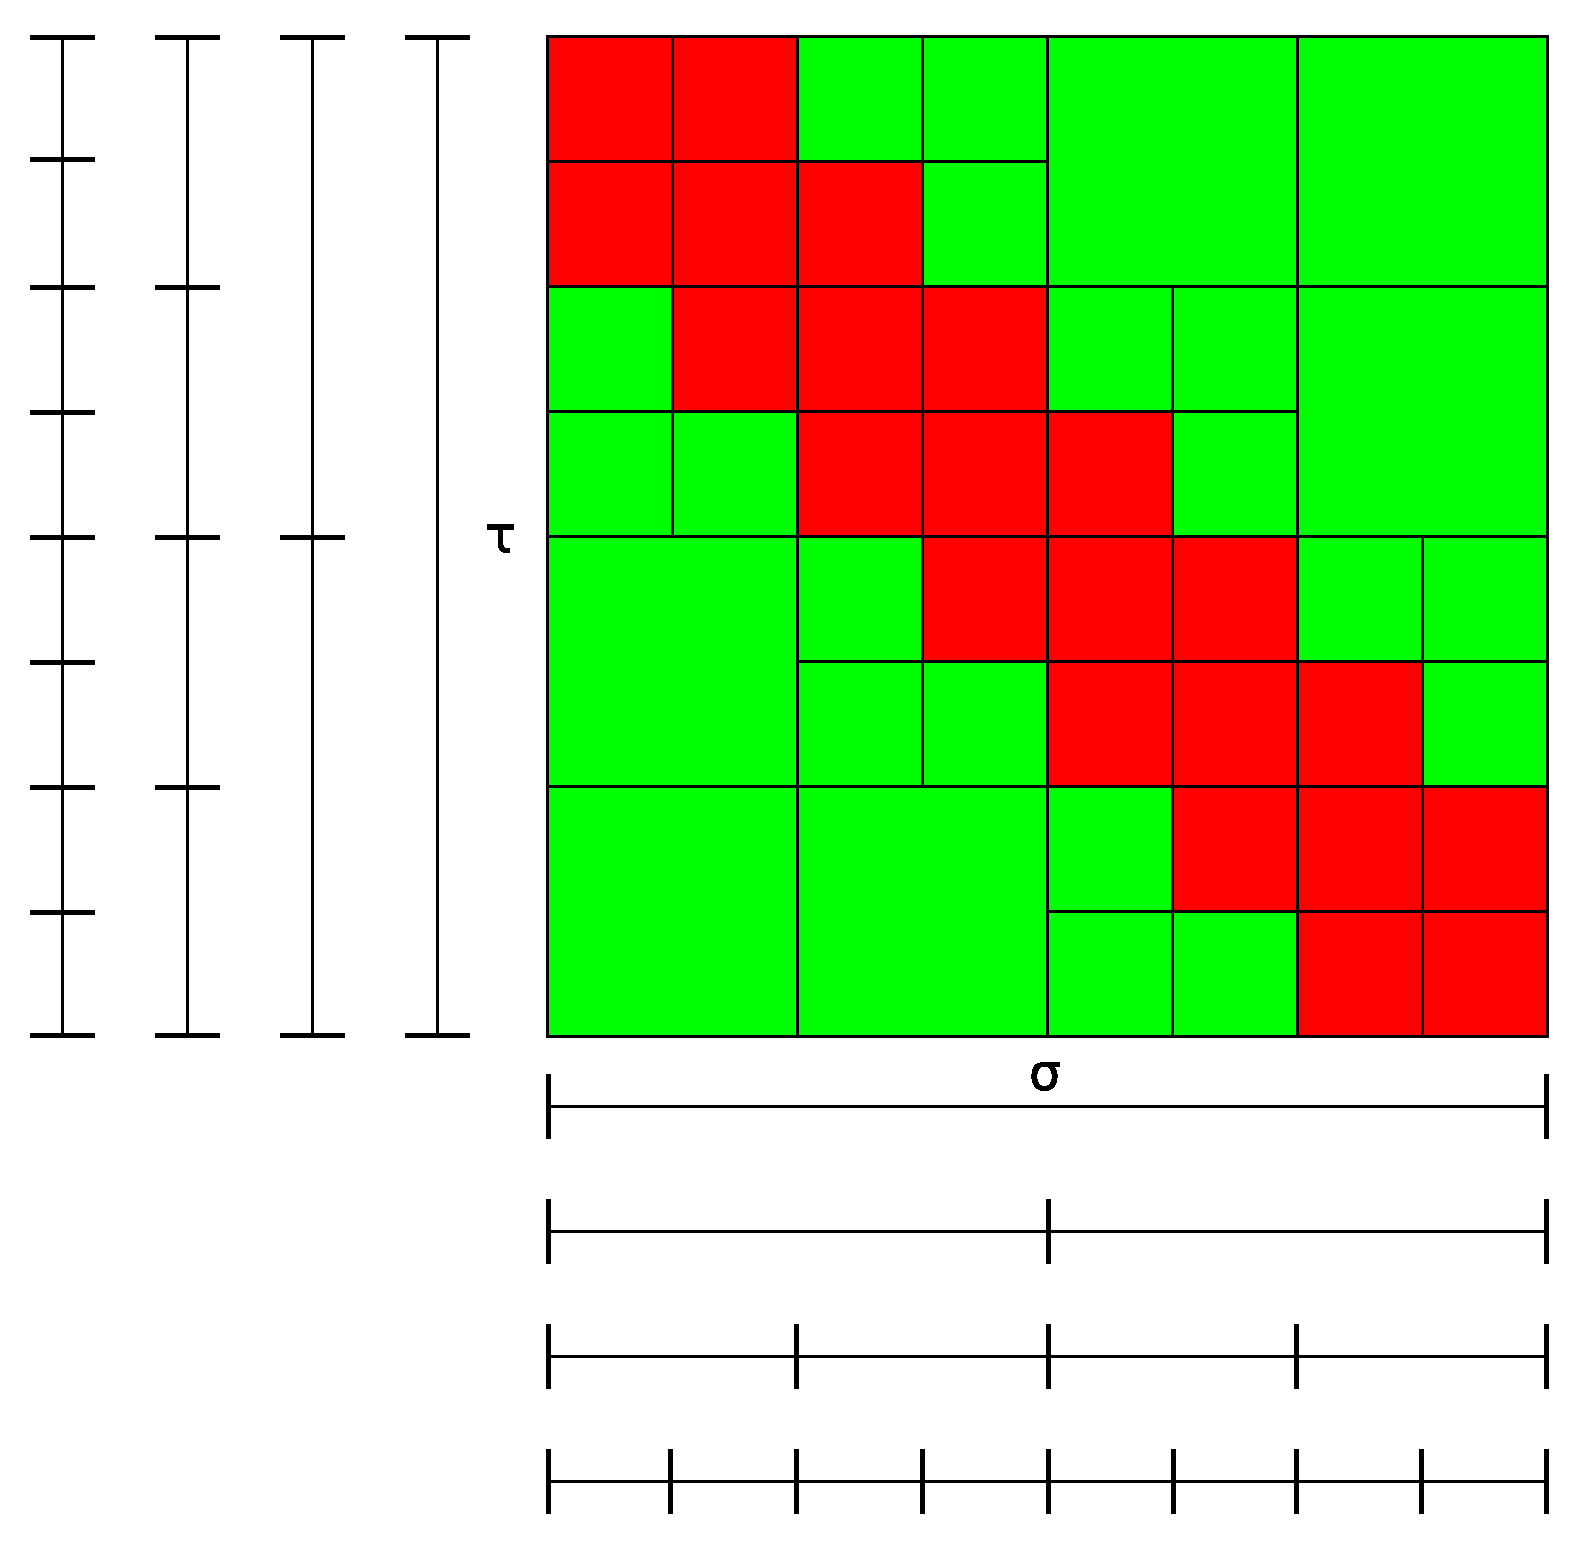
\includegraphics[width=.5\linewidth]{figures/fg-h2-matrix.pdf}\caption{Aufbau einer \(\mathcal{H}^2\)-Matrix aus Clusterbasen \( \tau \) und \( \sigma \)}
      \onslide<2>\centering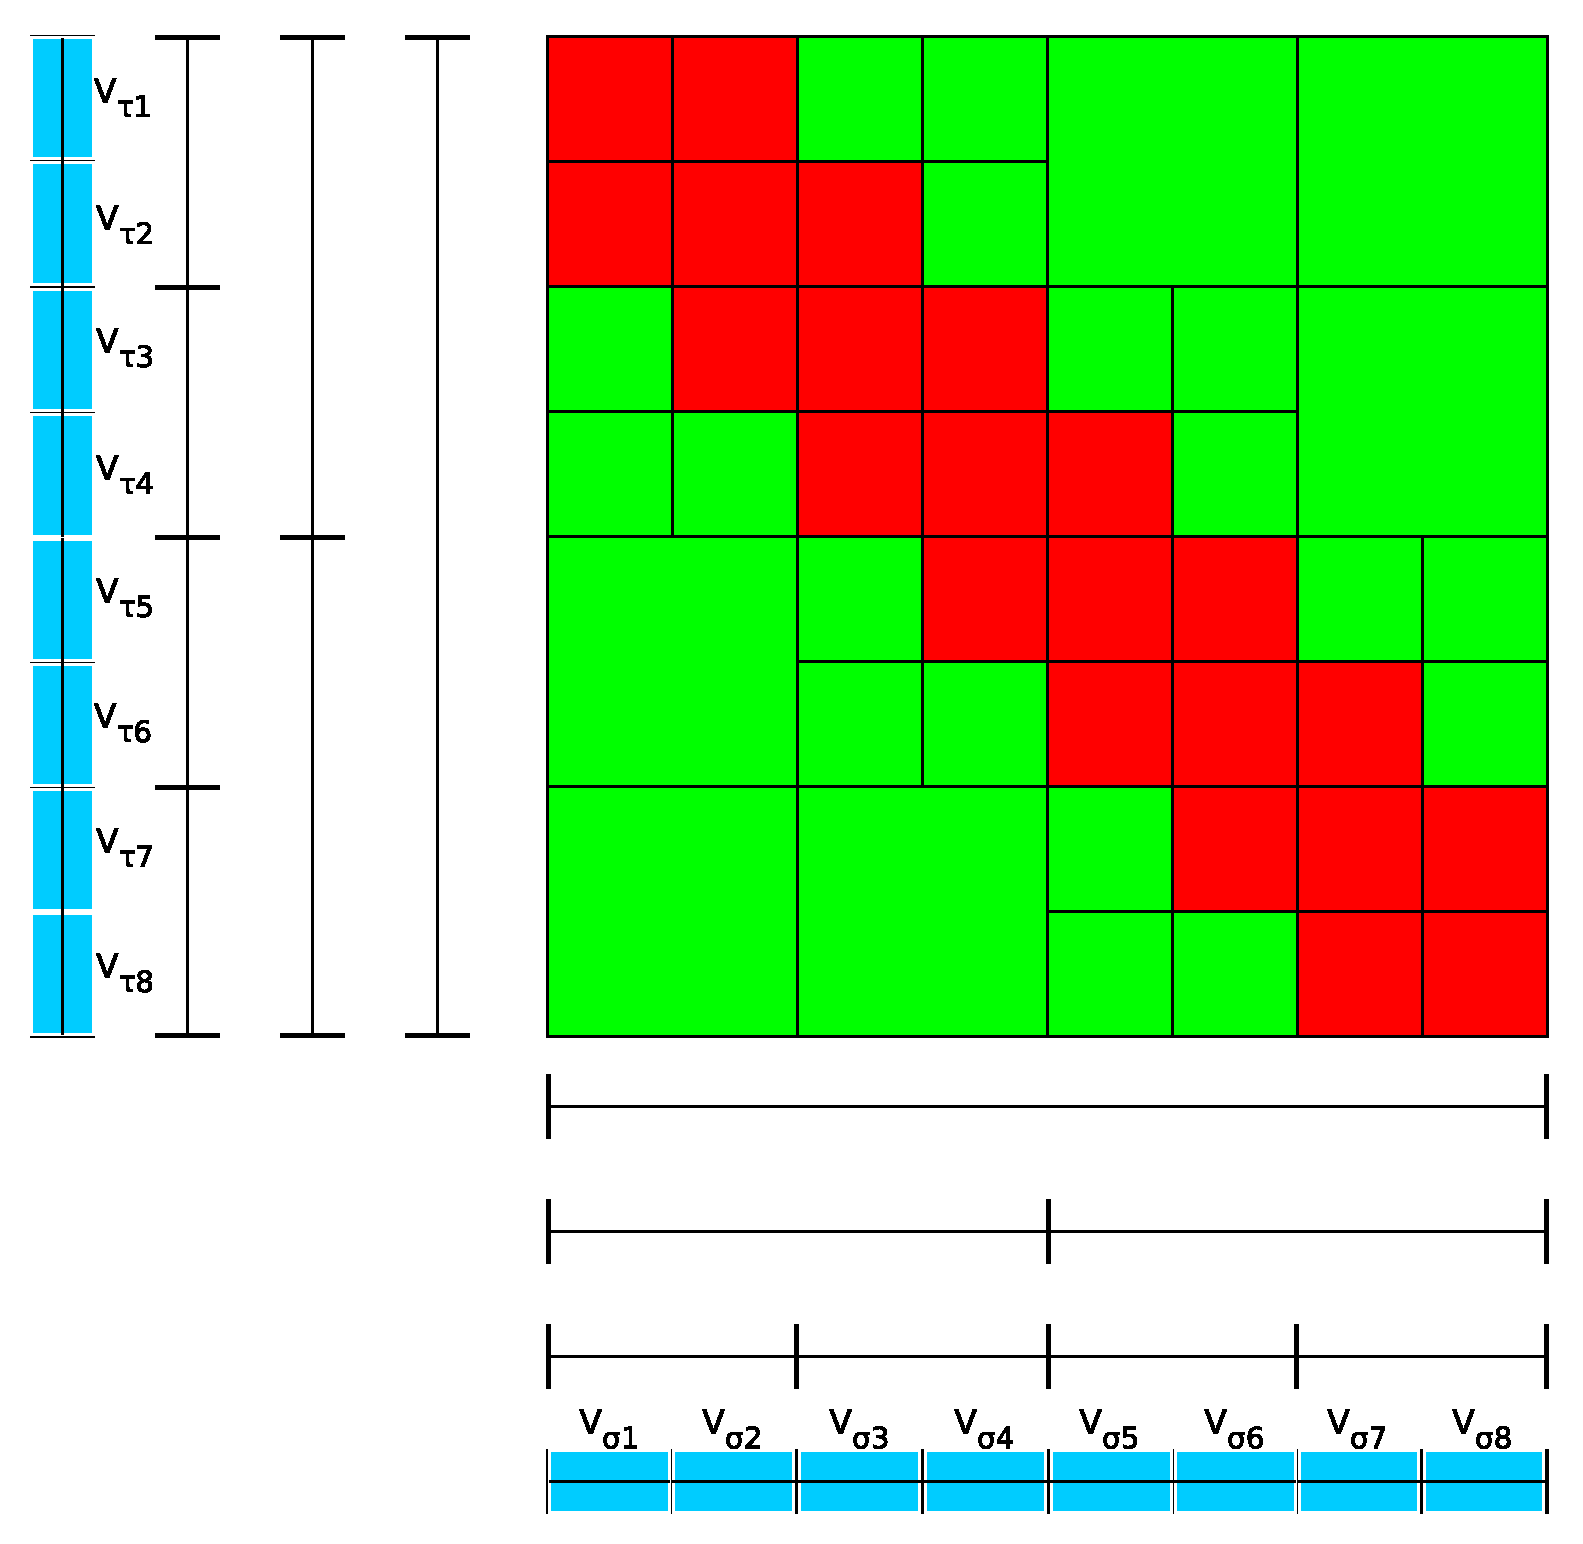
\includegraphics[width=.5\linewidth]{figures/fg-h2-leaf-matrices.pdf}\caption{Blattmatrizen der Clusterbasen \(\tau\) und \(\sigma\)}
      \onslide<3>\centering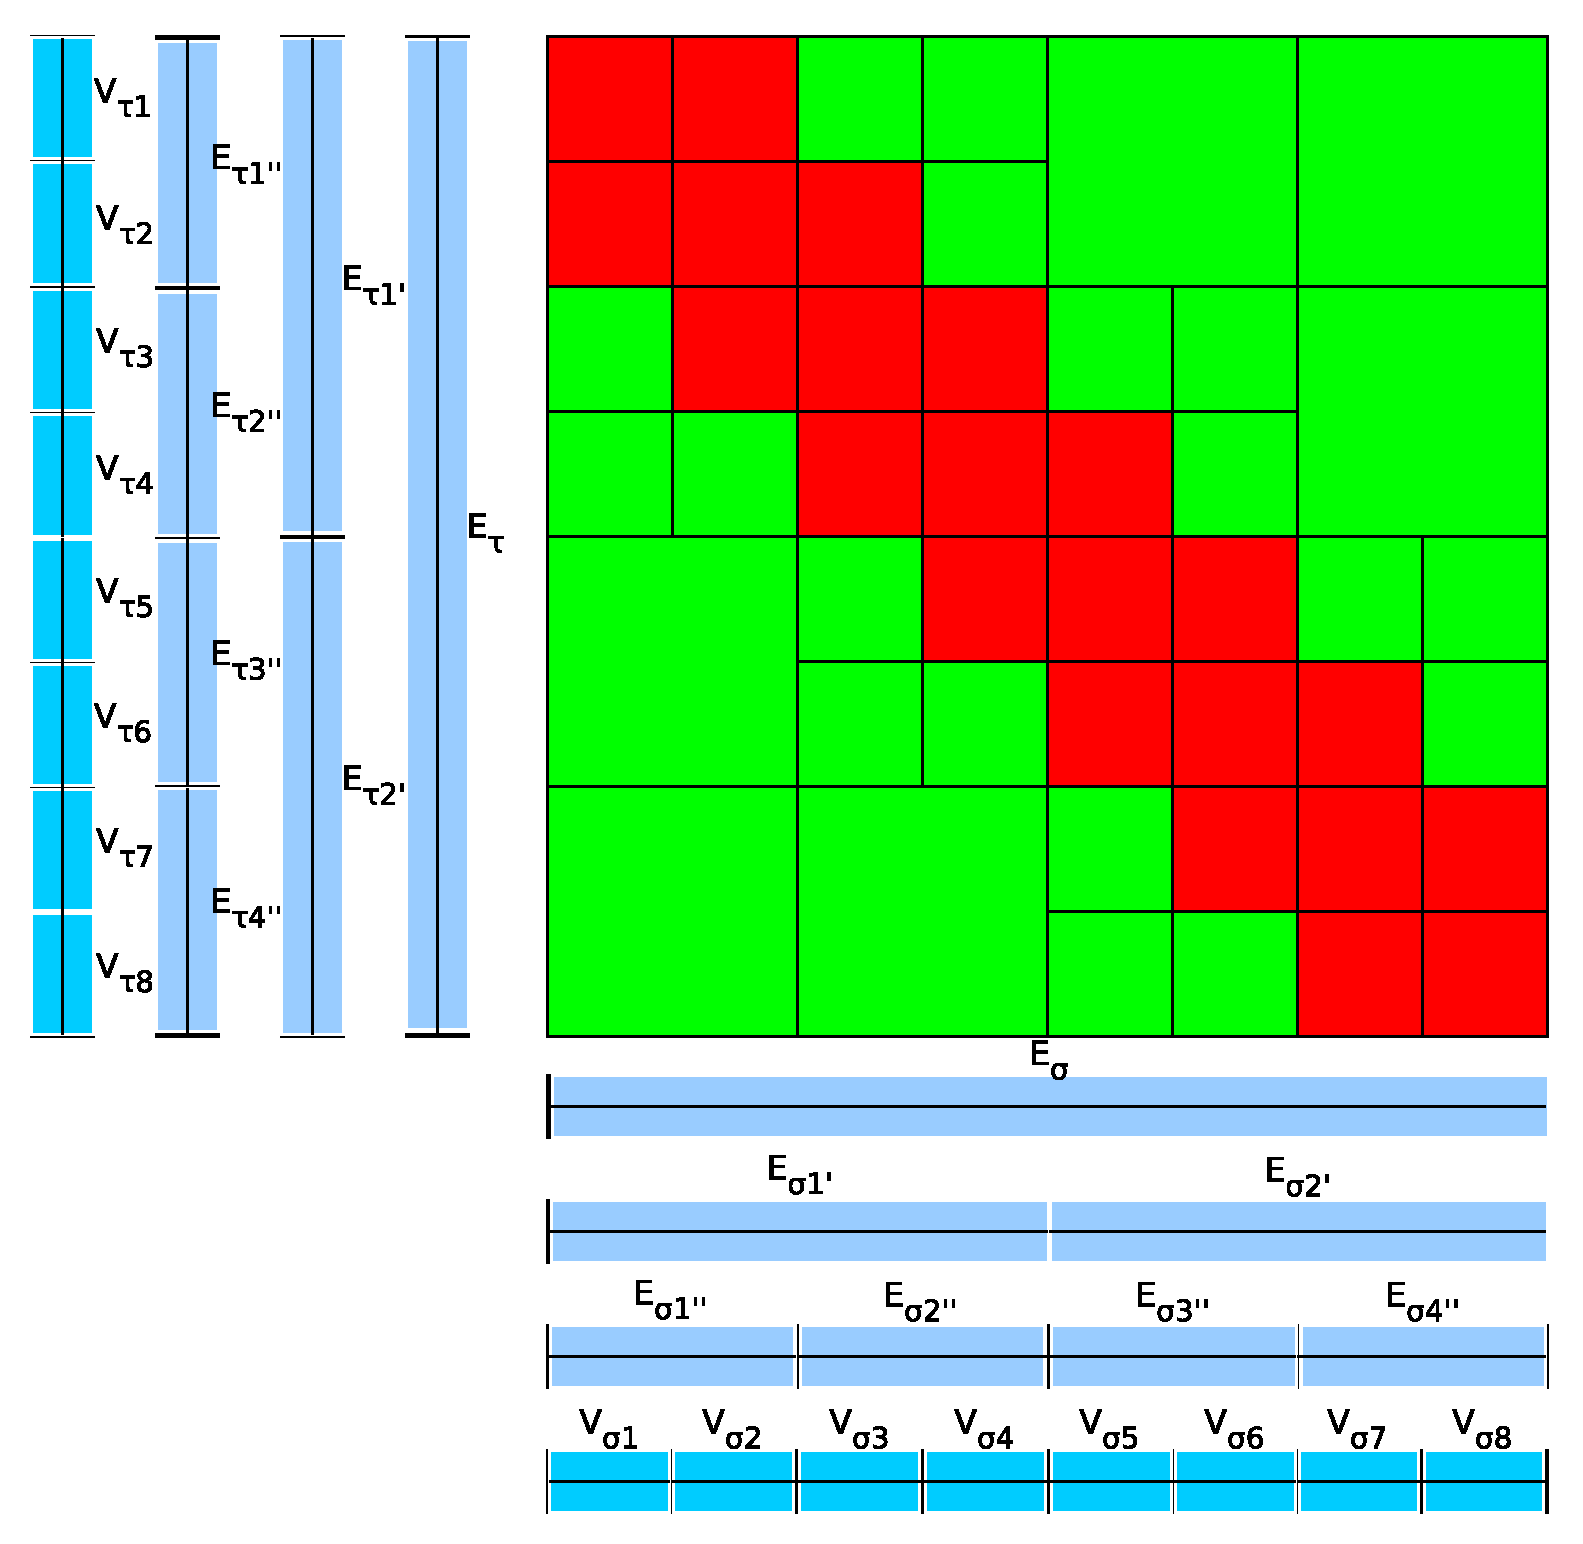
\includegraphics[width=.5\linewidth]{figures/fg-h2-transfer-matrices.pdf}\caption{Aufbau der Teilclusterbasen von \(\tau\) und \(\sigma\)}
      \onslide<4>\centering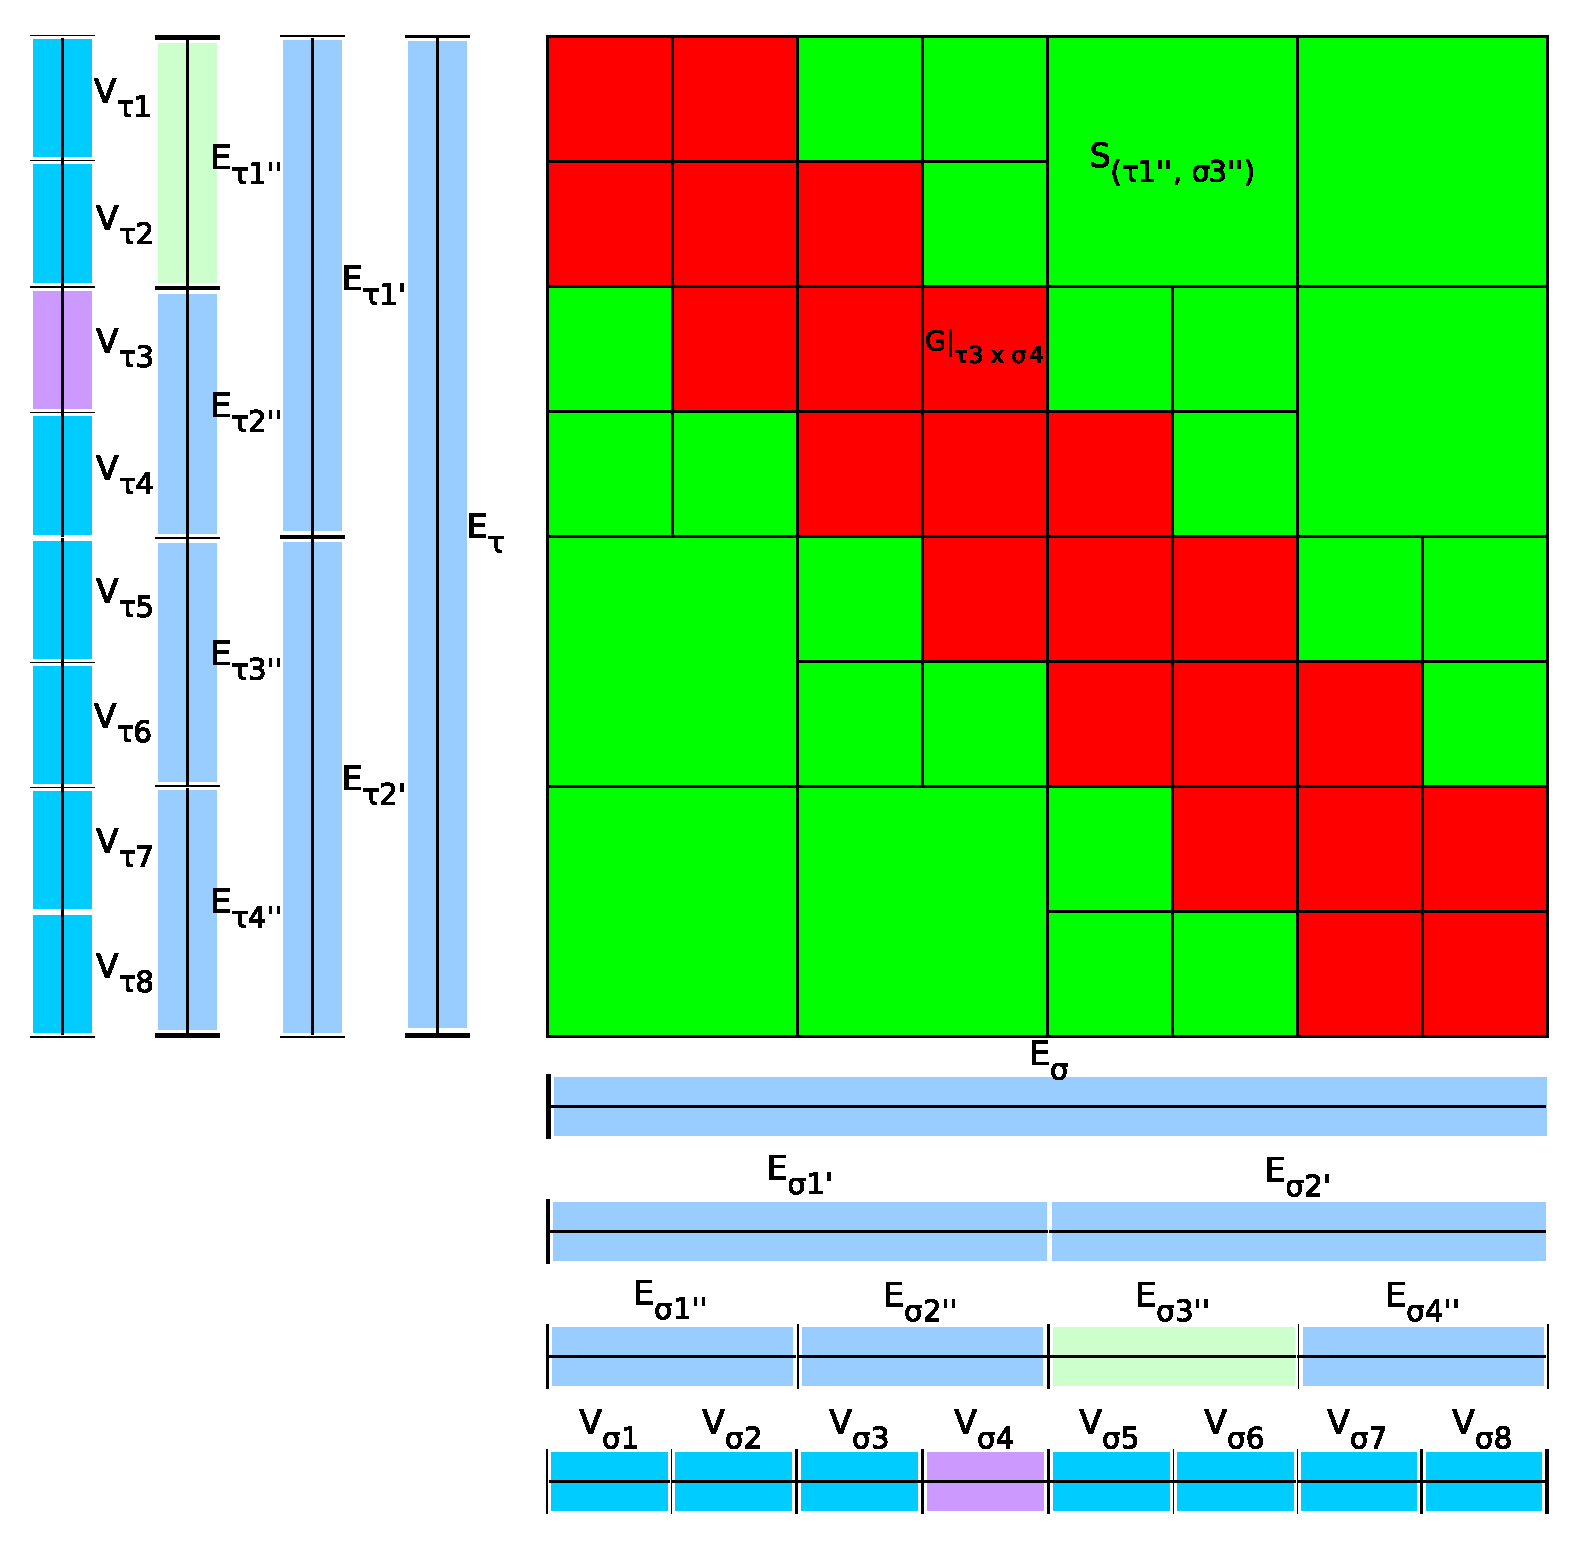
\includegraphics[width=.5\linewidth]{figures/fg-h2-near-far-field-matrices.pdf}\caption{Matrizen für zulässige und unzulässige Blöcke}
    \end{overprint}
  \end{figure}

  \footnotesize
  \let\thefootnote\relax\footnote{Wolfgang Hackbusch und Steffen B{\"o}rm.
  \href{https://link.springer.com/article/10.1007\%2Fs00607-002-1450-4?LI=true}{``Data-sparse approximation by adaptive \(\mathcal{H}^2\)-matrices''}. In:
   \textit{Computing} 69.1 (2002), S. 1-35.}
  \addtocounter{footnote}{-1}\let\thefootnote\svthefootnote\relax
  \normalsize
\end{frame}

\begin{frame}{\(\mathcal{H}^2\)-Matrizen}
  \begin{itemize}
    \item Sei \(\tilde{G}|_{\hat{\tau} \times \hat{\sigma}} =
    \begin{cases}
      V_{\tau} S_{\tau \sigma} V_{\sigma}^T & \tau \times \sigma \text{ zulässig} \\
      G|_{\hat{\tau} \times \hat{\sigma}}   & sonst
    \end{cases}\)
    \begin{itemize}
      \item Seien \(\hat{\tau}\) und \( \hat{\sigma}\) die Indexmengen von \(\tau\) und \(\sigma\)
    \end{itemize}
    \item \(V_{\tau}\) existiert, falls \(\tau\) ein Blatt ist
    \item Ansonsten gilt \(V_{\tau}|_{\hat{\tau} '} = V_{\tau '} E_{\tau '}\) für alle  \(\tau ' \in sons(\tau)\)
    \item \(V_{\sigma}\) ist analog definiert
  \end{itemize}

  \footnotesize
  \let\thefootnote\relax\footnote{Wolfgang Hackbusch und Steffen B{\"o}rm.
  \href{https://link.springer.com/article/10.1007\%2Fs00607-002-1450-4?LI=true}{``Data-sparse approximation by adaptive \(\mathcal{H}^2\)-matrices''}. In:
   \textit{Computing} 69.1 (2002), S. 1-35.}
  \addtocounter{footnote}{-1}\let\thefootnote\svthefootnote\relax
  \normalsize
\end{frame}

\begin{frame}{\(\mathcal{H}^2\)-Matrix-Vektor-Multiplikation}
  \begin{columns}
    \column{.30\linewidth}
      \begin{overprint}
        \onslide<1>
          \( y|_{\hat{\tau}} := \overbrace{V_{\tau} \underbrace{S_{\tau \sigma}
             \overbrace{V_{\sigma}^T
             x|_{\hat{\sigma}}}^{\textcolor{red}{\text{forward}}}}_{fastaddeval}}^{backward} \)
        \onslide<2>
          \( y|_{\hat{\tau}} := \overbrace{V_{\tau} \underbrace{S_{\tau \sigma}
             \textcolor{orange}{\hat{x}_\sigma}}_{\textcolor{red}{fastaddeval}}}^{backward} \)
        \onslide<3>
           \( y|_{\hat{\tau}} := \overbrace{V_{\tau}
              \textcolor{orange}{\hat{y}_\tau}}^{\textcolor{red}{backward}} \)
      \end{overprint}

    \column{.60\linewidth}
      \begin{overprint}
        \onslide<1>
          \begin{algorithm}[H]
            \SetAlFnt{\tiny}
            \SetKwProg{Proc}{}{}{}
            \Proc{forward\relax(\( \sigma \))}
            {
              \uIf{sons\( (s) = \emptyset \) \textbf{then}}
              {
                \( \hat{x}_{s} \leftarrow W_{s}^{*}x|_{\hat{s}} \) \;
              }
              \Else{
                \( \hat{x}_{s} \leftarrow 0 \) \;
                \ForAll{\( s' \in \text{sons}(s) \)}
                {
                  \textit{forward\relax(}\( W, \ s', \ x, \
                    \hat{x} \)\textit{)} \;
                  \( \hat{x}_{s} \leftarrow \hat{x}_{s} + F_{s'}^{*}
                     \hat{x}_{s'}\) \;
                }
              }
            }
          \end{algorithm}
        \onslide<2>
          \begin{algorithm}[H]
            \SetKwProg{Proc}{}{}{}
            \Proc{fastaddeval \\ \quad \small{(\( \alpha, \ G, \ b = (t, s), \ x, \
                                                   \hat{x}, \, \textbf{var } y, \hat{y}
                                                \))}}
            {
              \uIf{\( b \in \mathcal{L}^{+}_{\mathcal{I} \times \mathcal{J}}
                   \)}
              {
                \( \hat{y}_{t} \leftarrow \hat{y}_{t} + \alpha S_{b}\hat{x}_{s}
                \) \;
              }
              \uElseIf{\( b \in\mathcal{L}^{-}_{\mathcal{I} \times
                          \mathcal{J}} \)}
              {
                \( y|_{\hat{t}} \leftarrow y|_{\hat{t}} + \alpha
                   N_{b}x|_{\hat{s}} \) \;
              }
              \Else{
                \ForAll{\( b' \in \text{sons}(b)\)}
                {
                  \small{\textit{fastaddeval\relax(}\( \alpha, \ G, \ b', \ x, \
                                                                  \hat{x}, \ y, \
                                                                  \hat{y} \)\textit{)} \;}
                }
              }
            }
          \end{algorithm}
        \onslide<3>
          \begin{algorithm}[H]
            \SetKwProg{Proc}{}{}{}
            \Proc{backward\relax(\( V, \ t, \ \textbf{var } \hat{y}, \ y
                                                \))}
            {
              \eIf{sons\( (t) = \emptyset \) \textbf{then}}
              {
                \( y|_{\hat{t}} \leftarrow y|_{\hat{t}} + V_{t}\hat{y}_{t} \) \;
              }
              {
                \ForAll{\( s' \in \text{sons}(s) \)}
                {
                \( \hat{y}_{t'} \leftarrow \hat{y}_{t'} + E_{t'} \hat{y}_{t}\) \;
                  \textit{backward\relax(}\( V, \ t', \ \hat{x}, \ x
                  \)\textit{)} \;
              }
            }
          }
        \end{algorithm}
      \end{overprint}
  \end{columns}

  \footnotesize
  \let\thefootnote\relax\footnote{Wolfgang Hackbusch und Steffen B{\"o}rm.
  \href{https://link.springer.com/article/10.1007\%2Fs00607-002-1450-4?LI=true}{``Data-sparse approximation by adaptive \(\mathcal{H}^2\)-matrices''}. In:
   \textit{Computing} 69.1 (2002), S. 1-35.}
  \addtocounter{footnote}{-1}\let\thefootnote\svthefootnote\relax
  \normalsize
\end{frame}

\section{Sauter-Schwab Quadratur}

\begin{frame}{Sauter-Schwab Quadratur}
  \begin{itemize}
    \item Vier Fälle von Integralen, abhängig von den entsprechenden 
          Dreieckspaaren \( \Delta_{i}, \ \Delta_{j} \) der Triangulation:
    \begin{enumerate}
        \item \( \Delta_{i} \) und \( \Delta_{j} \) sind disjunkt, also \(
                 \Delta_{i} \cap \Delta_{j} = \emptyset \).
        \item \( \Delta_{i} \) und \( \Delta_{j} \) teilen sich einen Vertex \(
                 v \in \mathbb{R}^{d} \), also \( \Delta_{i} \cap \Delta_{j} = 
                 \{ v \} \).
        \item \( \Delta_{i} \) und \( \Delta_{j} \) teilen sich eine Kante
              \( \{ v_{1}, \ v_{2} \} \in \mathbb{R}^{d} \times \mathbb{R}^{d} 
              \), also \( \Delta_{i} \cap \Delta_{j} = \{ v_{1}, \ v_{2} \} \).
        \item \( \Delta_{i} \) und \( \Delta_{j} \) sind identisch, also \(
                 \Delta_{i} = \Delta_{i} \cap \Delta_{j} = \Delta_{j} \).
    \end{enumerate}
    \item Auswertung reduziert sich auf (eine) unterschiedliche (Anzahl von)
          Quadraturpunkten und Permutation der Dreiecksvertices zueinander
  \end{itemize}

  \footnotesize
  \let\thefootnote\relax\footnote{S. A. Sauter und C. Lage.
  \href{https://link.springer.com/article/10.1007\%2Fs00211-015-0757-y}{
  ``On the efficient computation of singular and nearly singular surface 
  integrals arising in 3D-Galerkin BEM''}. In:   \textit{Zeitschrift f\"ur 
  angewandte Mathematik und Mechanik } 76 (1996), S. 273-275.}
  \addtocounter{footnote}{-1}\let\thefootnote\svthefootnote\relax
  \normalsize
\end{frame}

\section{GCA-Methode}

\begin{frame}{GCA-Methode}
  \begin{itemize}
    \item Sei ein zulässiger Block \(b = (\tau \times \sigma)\) gegeben
    \item Algebraische Interpolation in zulässigen Blättern
    \begin{itemize}
      \item Greens zweite Identität, Quadratur und adaptive Kreuzapproximation
      \item \visible<2->{\(\mathfrak{I}_{\tau} = V_{\tau}P_{\tau}, \qquad
                           \mathfrak{I}_{\sigma} = W_{\sigma}P_{\sigma}\)}
      \item \visible<2->{\(V_{\tau} \in \mathbb{R}^{\tau \times \tilde{\tau}},
                           \qquad W_{\sigma} \in \mathbb{R}^{\sigma \times
                           \tilde{\sigma}}\): \glqq Interpolationspolynome \grqq}
      \item \visible<2->{\(P_{\tau} \in \mathbb{R}^{\tilde{\tau} \times \tau},
                           \qquad P_{\sigma} \in \mathbb{R}^{\tilde{\sigma}
                           \times \sigma}\): \glqq Interpolationpunkte \grqq}
      \item \visible<2->{\(\tilde{\tau} \subseteq \tau, \qquad, \tilde{\sigma}
                           \subseteq \sigma\)}
      \item \visible<3->{\(G|_{\tau \times \sigma} \approx
                           \mathfrak{I}_{\tau} G|_{\tau \times \sigma}
                           \mathfrak{I}_{\sigma}^{*} =
                           V_{\tau} G|_{\tilde{\tau} \times \tilde{\sigma}}
                           W_{\sigma}^{*}\)}
    \end{itemize}
    \item \visible<4->{Adaptive Kreuzapproximation in Nicht-Blättern}
  \end{itemize}

  \footnotesize
  \let\thefootnote\relax\footnote{Steffen Börm und Sven Christophersen.
  \href{https://link.springer.com/article/10.1007\%2Fs00211-015-0757-y}{
  ``Approximation of integral operators by Green quadrature and nested cross 
  approximation''}. In:   \textit{Numerische Mathematik} 133.3 (2016), S. 
  409-442, 2016.}
  \addtocounter{footnote}{-1}\let\thefootnote\svthefootnote\relax
  \normalsize
\end{frame}

\section{GPUs}

\begin{frame}{GPUs}
  \begin{columns}
    \column{0.45\linewidth}
      \begin{itemize}
        \item Graphics Processing Unit (GPU) ist ein auf Bildverarbeitung
              spezialisierter Prozessor
        \begin{itemize}
          \item Schnelle Gleitkommaoperationen
          \item Vektorisierte Architektur
        \end{itemize}
        \item Entwicklung von GPUs durch Videospielindustrie stark
              vorangetrieben
        \item Sehr günstig dank Massenproduktion
      \end{itemize}
    \column{0.45\linewidth}
      \begin{figure}
        \centering
        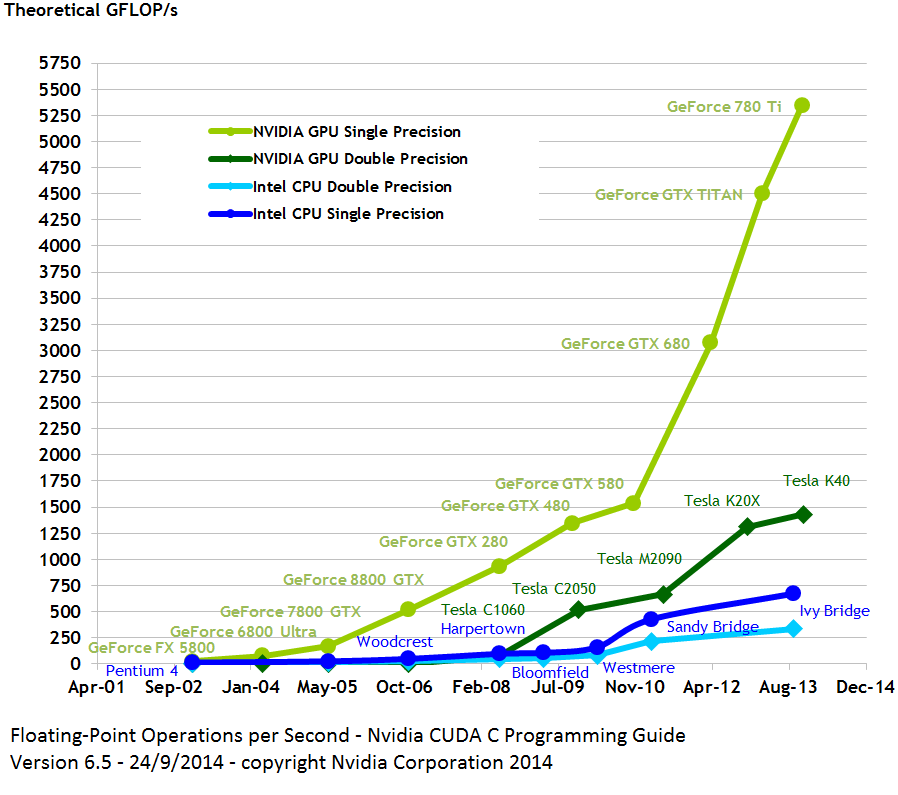
\includegraphics[width=\linewidth]{figures/fg-flops.png}
        \caption{Theoretische Verarbeitungsgeschwindigkeit von
                 Gleitkommaoperationen verschiedener
                 Architekturen\footnotemark[1]}
      \end{figure}
  \end{columns}

  \footnotetext[1]{\url{https://scs.senecac.on.ca/~gpu610/pages/images/flops.png}}
\end{frame}

\begin{frame}{GPUs}
  \begin{figure}
    \centering
    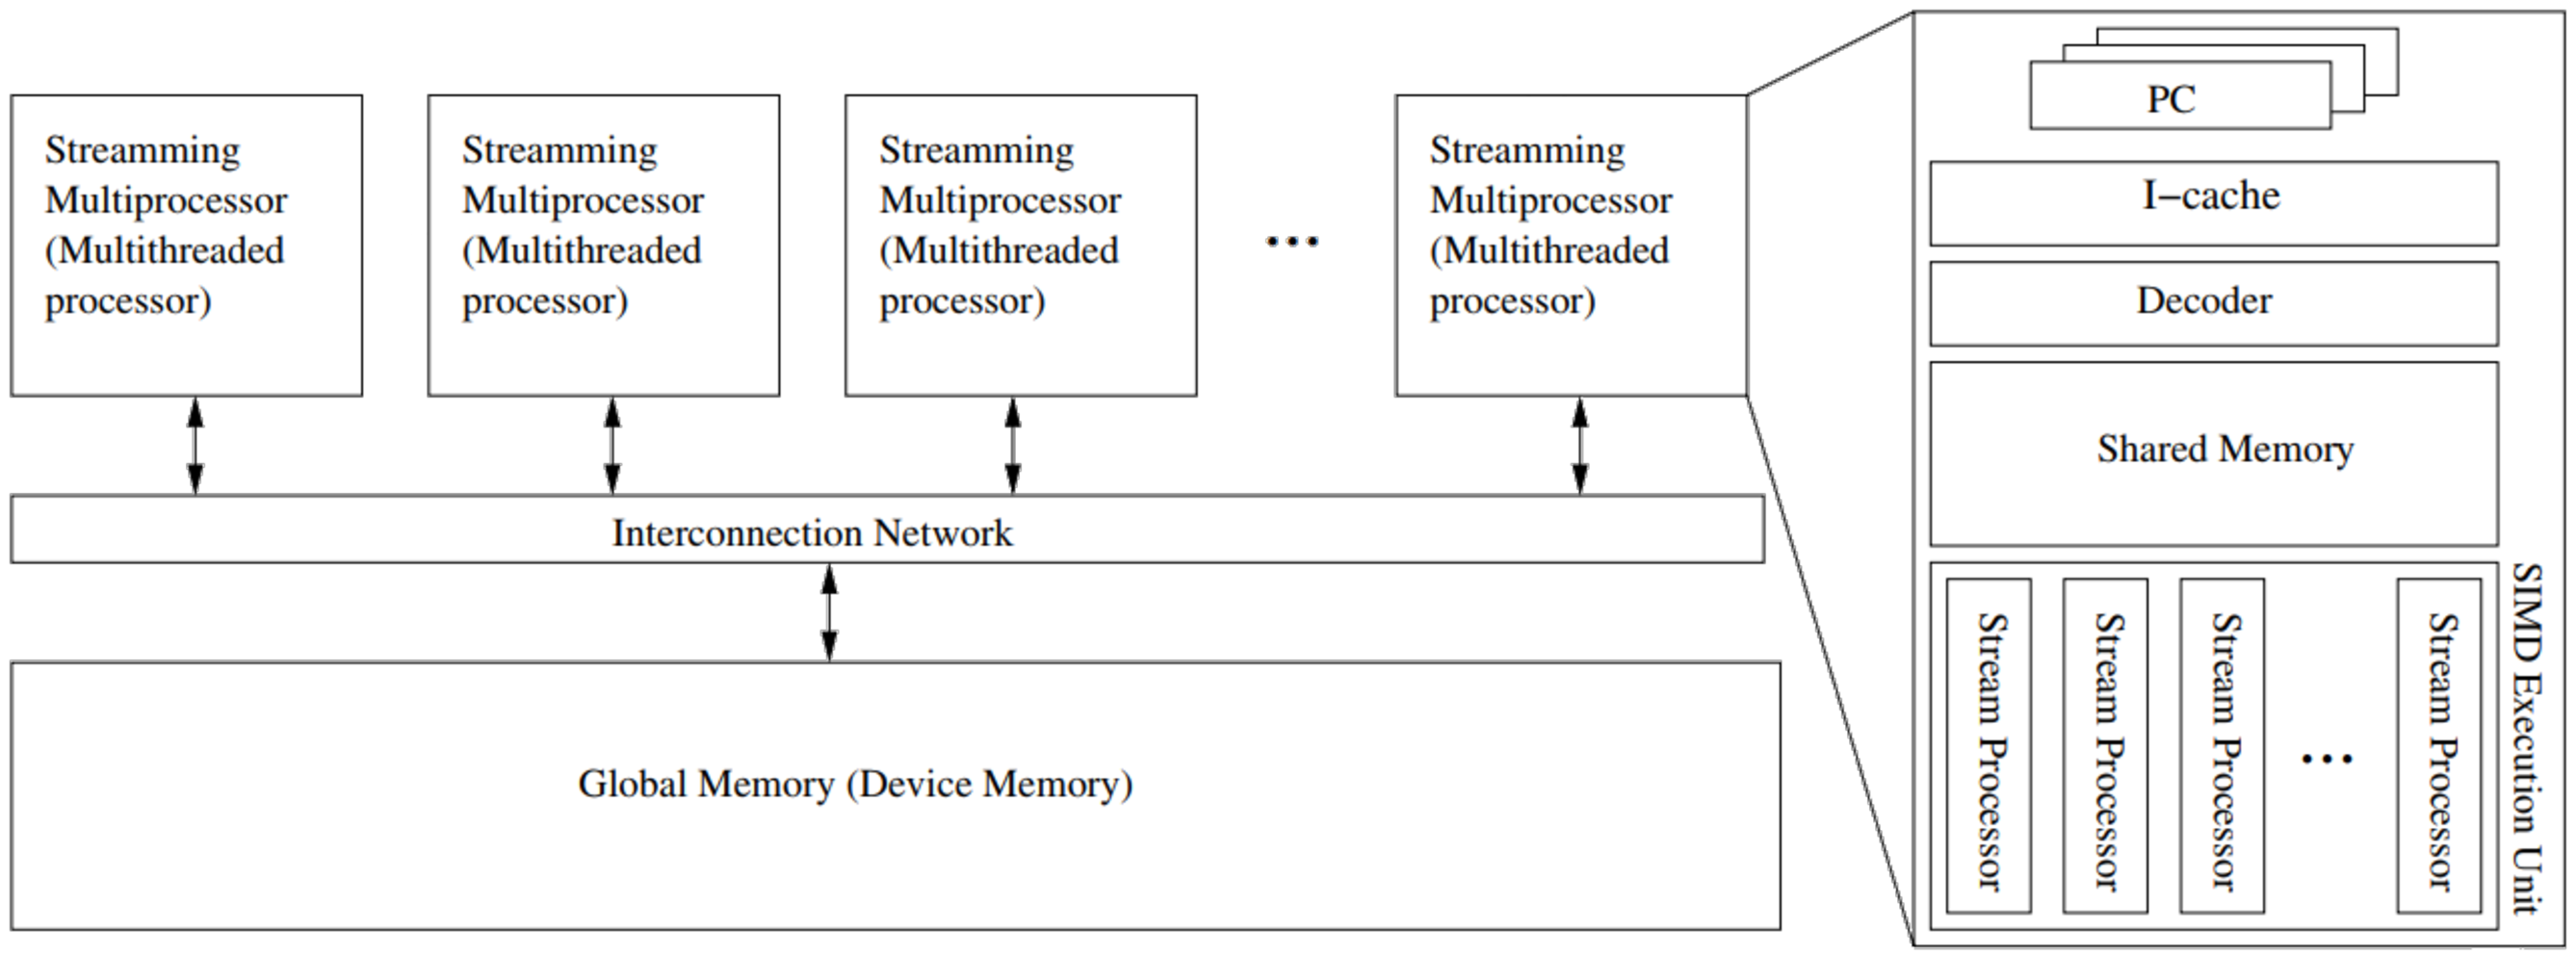
\includegraphics[width=\linewidth]{figures/fg-gpu_architecture.pdf}
    \caption{Architektur einer Graphikkarte}
  \end{figure}

  \footnotesize
  \let\thefootnote\relax\footnote{Sunpyo Hong und Hyesoon Kim.
  \href{https://link.springer.com/article/10.1007\%2Fs00211-015-0757-y}{
  ``An analytical model for a GPU architecture with memory-level and thread-level parallelism awareness''}. In:   \textit{ACM SIGARCH Computer 
  Architecture News}. Bd. 37. 3. 2009, S. 152-163.}
  \addtocounter{footnote}{-1}\let\thefootnote\svthefootnote\relax
  \normalsize
\end{frame}

\section{OpenCL}

\begin{frame}{OpenCL}
  \begin{itemize}
    \item Framework zum Programmieren von/auf unterschiedlichen
          Hardwarearchitekturen
    \begin{itemize}
      \item Field Programmable Gate Arrays (FPGAs)
      \item Digitaler Signalprozessoren (DSPs)
      \item CPUs
      \item GPUs
    \end{itemize}
  \end{itemize}

  \footnotesize
  \let\thefootnote\relax\footnote{Lee Howes. \href{https://www.khronos.org/registry/OpenCL/specs/opencl-2.0.pdf}{\textit{The OpenCL Specifictaion}}. Document Revision: 23. Khronos OpenCL Working Group. Nov. 2015.}
  \addtocounter{footnote}{-1}\let\thefootnote\svthefootnote\relax
  \normalsize
\end{frame}

\begin{frame}{OpenCL}
  \begin{figure}
    \centering
    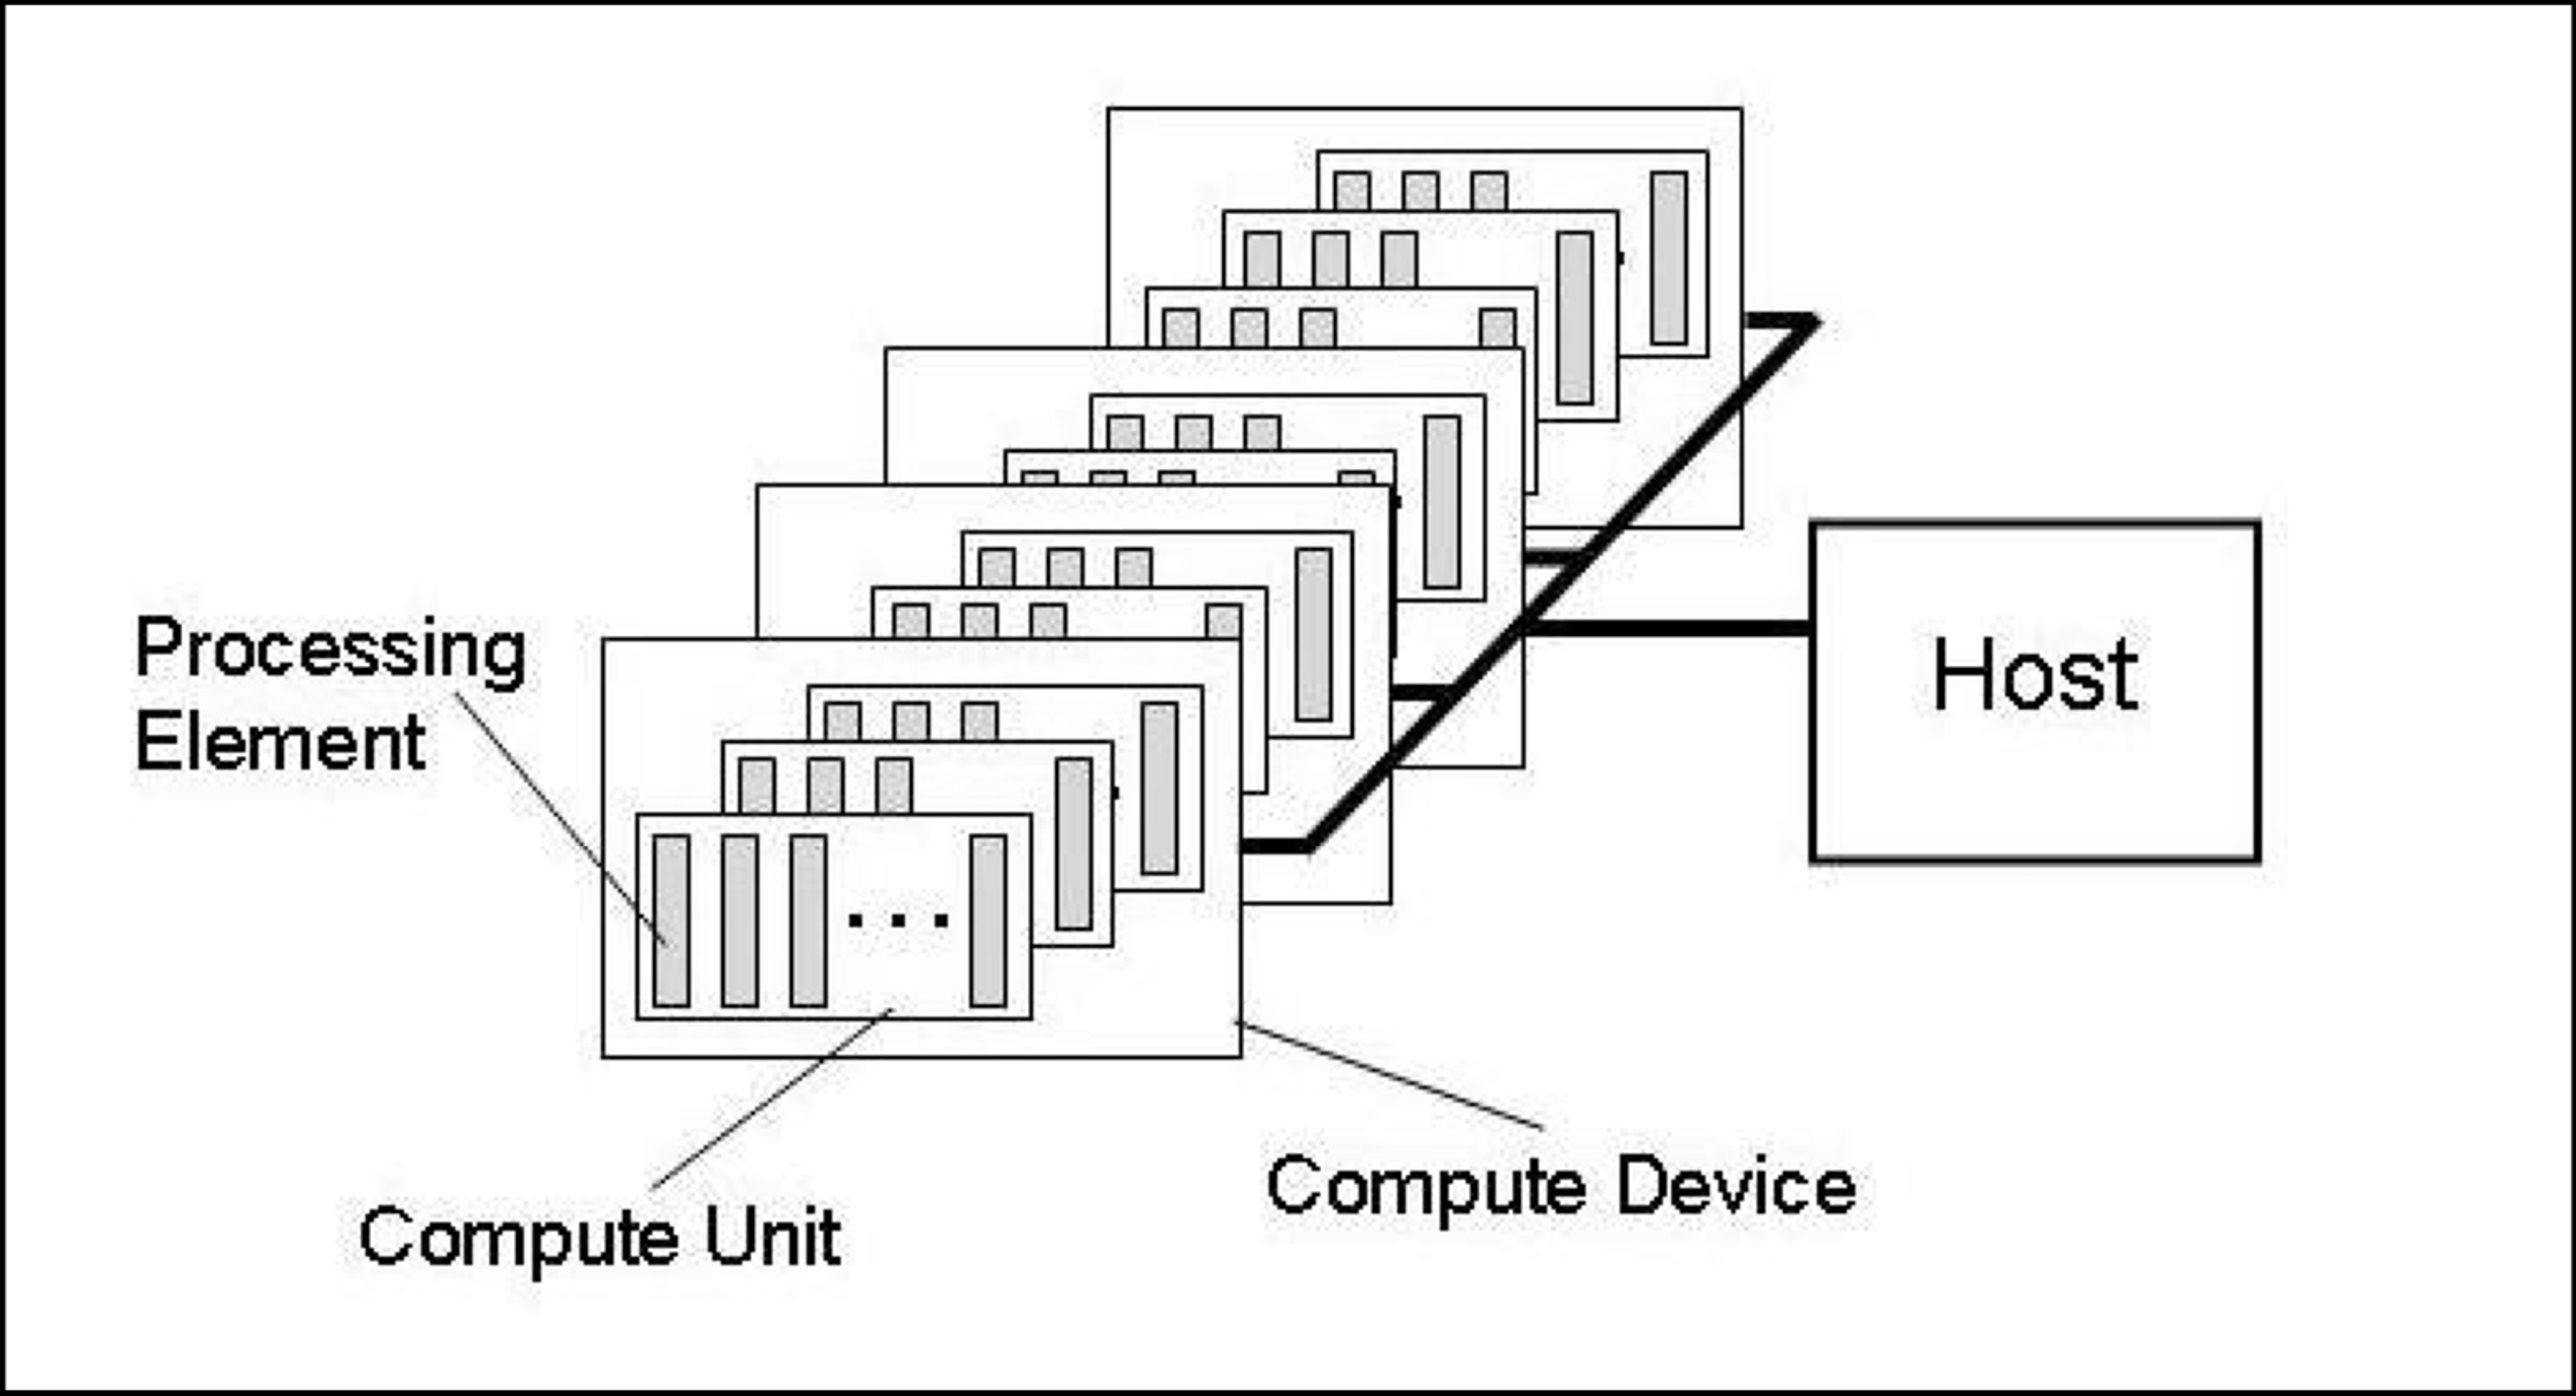
\includegraphics[width=.9\linewidth]{figures/fg-opencl-platform-model.pdf}
    \caption{Das Platformmodell von OpenCL}
  \end{figure}

  \footnotesize
  \let\thefootnote\relax\footnote{Lee Howes. \href{https://www.khronos.org/registry/OpenCL/specs/opencl-2.0.pdf}{\textit{The OpenCL Specifictaion}}. Document Revision: 23. Khronos OpenCL Working Group. Nov. 2015.}
  \addtocounter{footnote}{-1}\let\thefootnote\svthefootnote\relax
  \normalsize
\end{frame}

\begin{frame}{OpenCL}
  \begin{figure}
    \centering
    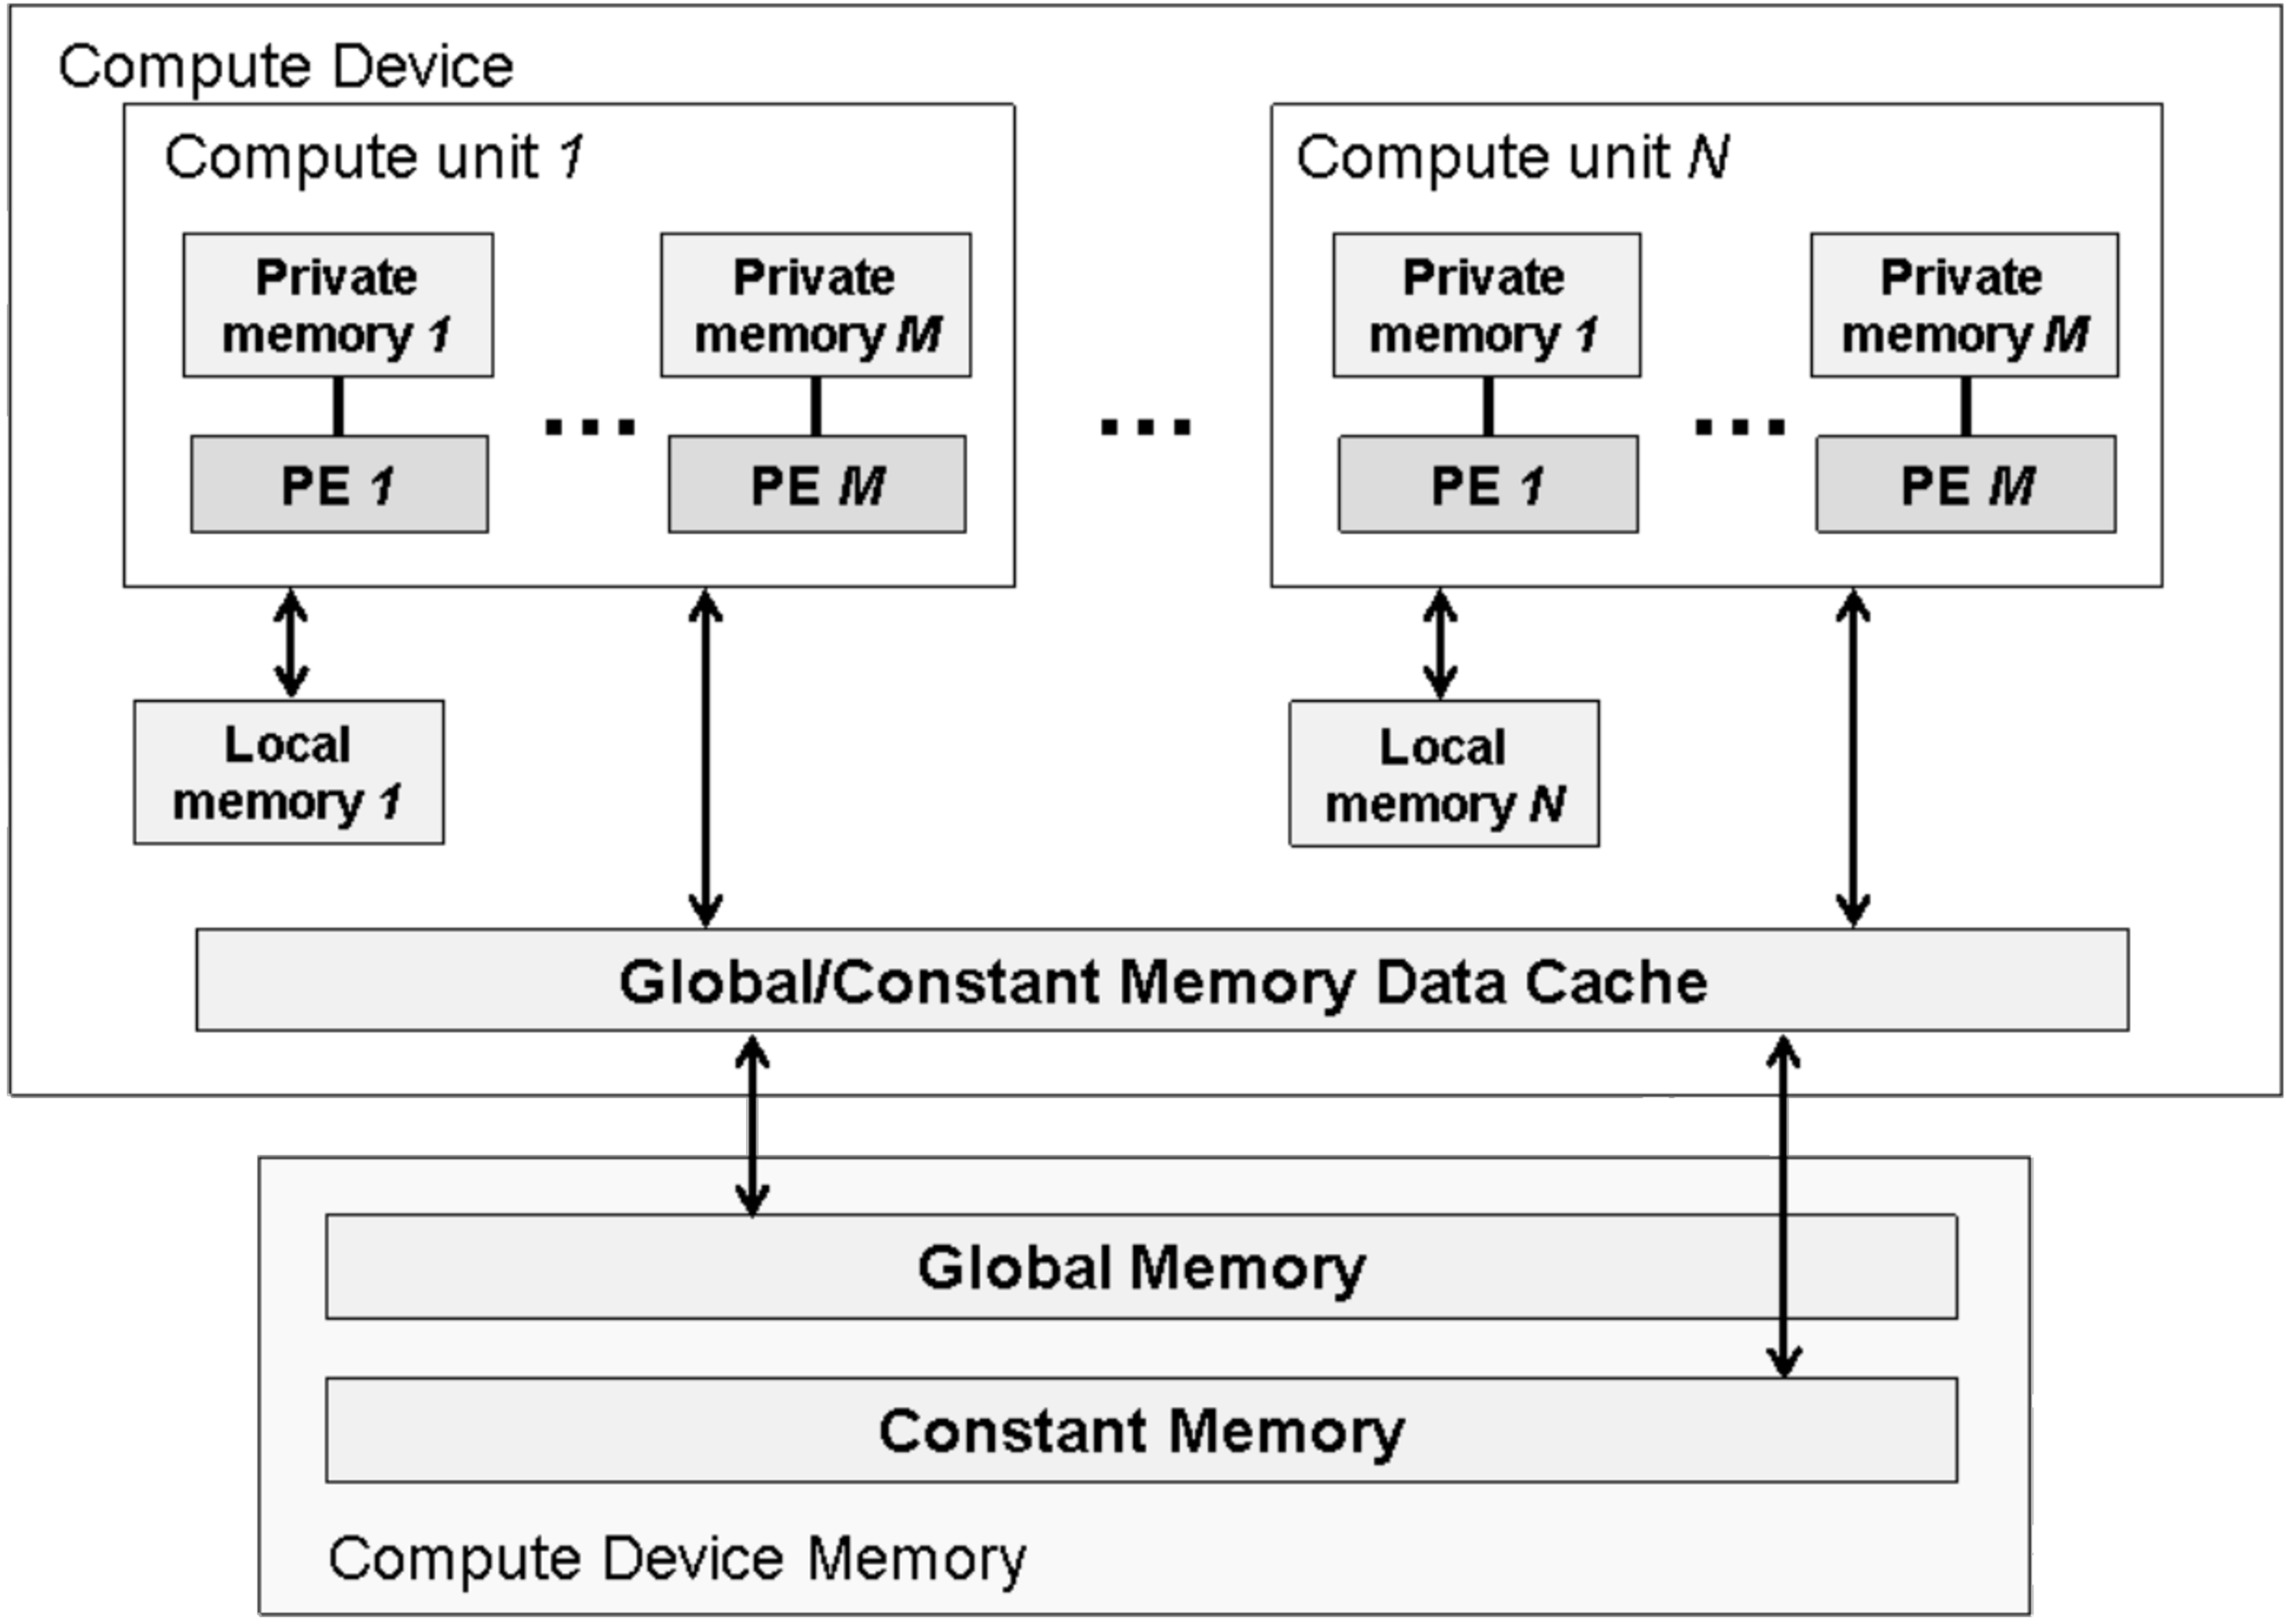
\includegraphics[width=.75\linewidth]{figures/fg-opencl-memory-model.pdf}
    \caption{Das Speichermodell von OpenCL}
  \end{figure}

  \footnotesize
  \let\thefootnote\relax\footnote{Lee Howes. \href{https://www.khronos.org/registry/OpenCL/specs/opencl-2.0.pdf}{\textit{The OpenCL Specifictaion}}. Document Revision: 23. Khronos OpenCL Working Group. Nov. 2015.}
  \addtocounter{footnote}{-1}\let\thefootnote\svthefootnote\relax
  \normalsize
\end{frame}

\begin{frame}{OpenCL}
  \begin{figure}
    \centering
    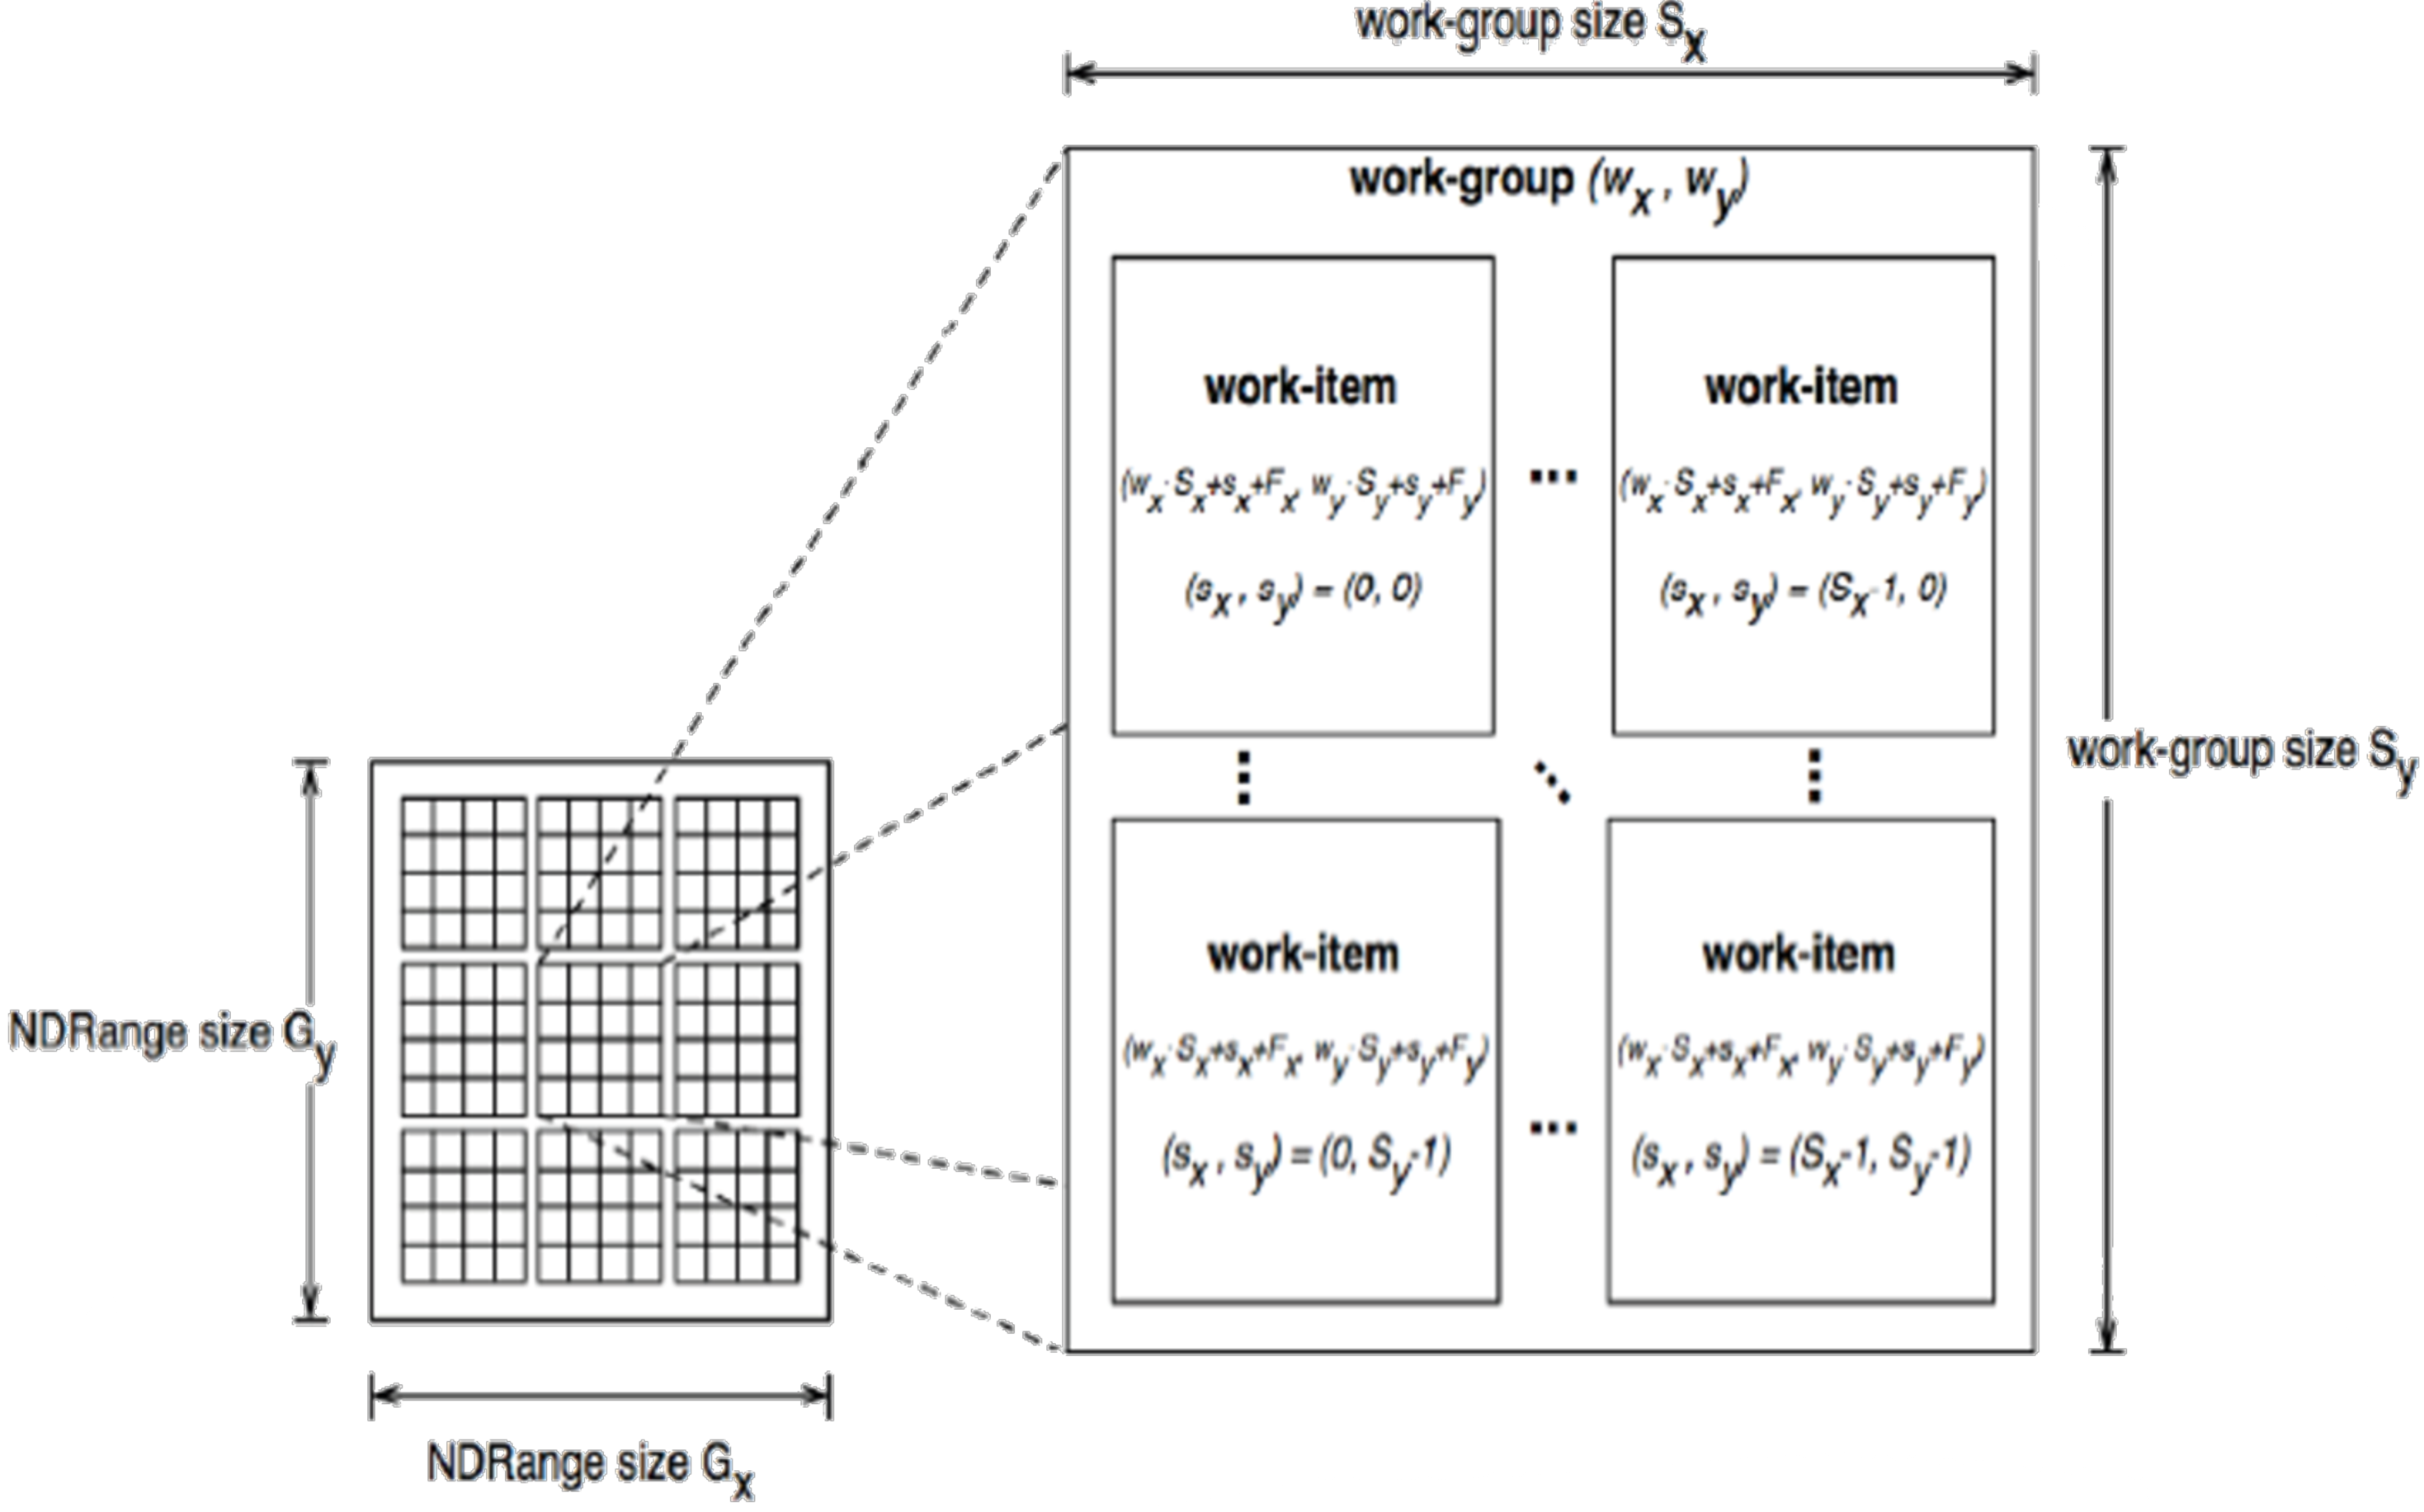
\includegraphics[width=.75\linewidth]{figures/fg-opencl-execution-model.pdf}
    \caption{Das Ausführungsmodell von OpenCL}
  \end{figure}

  \footnotesize
  \let\thefootnote\relax\footnote{Lee Howes. \href{https://www.khronos.org/registry/OpenCL/specs/opencl-2.0.pdf}{\textit{The OpenCL Specifictaion}}. Document Revision: 23. Khronos OpenCL Working Group. Nov. 2015.}
  \addtocounter{footnote}{-1}\let\thefootnote\svthefootnote\relax
  \normalsize
\end{frame}

\begin{frame}[fragile]{OpenCL}
  \begin{lstlisting}[style=CStyle]
  kernel void vec_inc(const size_t n,
                      global float *a,
                      const float b)
  {
    const size_t gid = get_global_id(0);

    if(gid >= n)
      return;

    a[gid] += b;
  }
  \end{lstlisting}
\end{frame}
\section{3 Phasen-fastaddeval}

\begin{frame}{Idee}
  \begin{columns}
    \column{.5\linewidth}
      \begin{itemize}
        \item Berechne reproduzierbare Matrizen nur bei Bedarf:
        \item \(S_{b} = P_{\tau}G|_{\tau \times \sigma} P_{\sigma}^{*}\)
        \begin{itemize}
          \item Permutierte Eintr\"age der Galerkin-Diskretisierung
          \item Eintr\"age bestehen nur aus einem Typ von
                Integralen
        \end{itemize}
        \item \(G|_{\hat{\tau} \times \hat{\sigma}}\)
        \begin{itemize}
          \item Eintr\"age der Galerkin-Diskretisierung
          \item Eintr\"age bestehen aus allen Typen von Integralen
        \end{itemize}
      \end{itemize}
    \column{.5\linewidth}
      \begin{algorithm}[H]
        \SetKwProg{Proc}{}{}{}
        \Proc{fastaddeval \newline \quad \small{(\( \alpha, \ G, \ b = (t, s), \ x, \
                                              \hat{x}, \, \textbf{var } y,
                                              \hat{y} \))}}
        {
          \uIf{\( b \in \mathcal{L}^{+}_{\mathcal{I} \times \mathcal{J}}
               \)}
          {
            \( \hat{y}_{t} \leftarrow \hat{y}_{t} + \alpha S_{b}\hat{x}_{s}
            \) \;
          }
          \uElseIf{\( b \in\mathcal{L}^{-}_{\mathcal{I} \times
                      \mathcal{J}} \)}
          {
            \( y|_{\hat{t}} \leftarrow y|_{\hat{t}} + \alpha
               N_{b}x|_{\hat{s}} \) \;
          }
          \Else{
            \ForAll{\( b' \in \text{sons}(b)\)}
            {
              \scriptsize{\textit{fastaddeval\relax(}\( \alpha, \ G, \ b', \ x, \
                                                   \hat{x}, \ y, \ \hat{y}
                                                \)\textit{)} \;}
            }
          }
        }
      \end{algorithm}
  \end{columns}
\end{frame}

\begin{frame}{Vorbereitung}\vfill
  \begin{figure}
    \begin{overprint}
      \onslide<1>
        \centering
        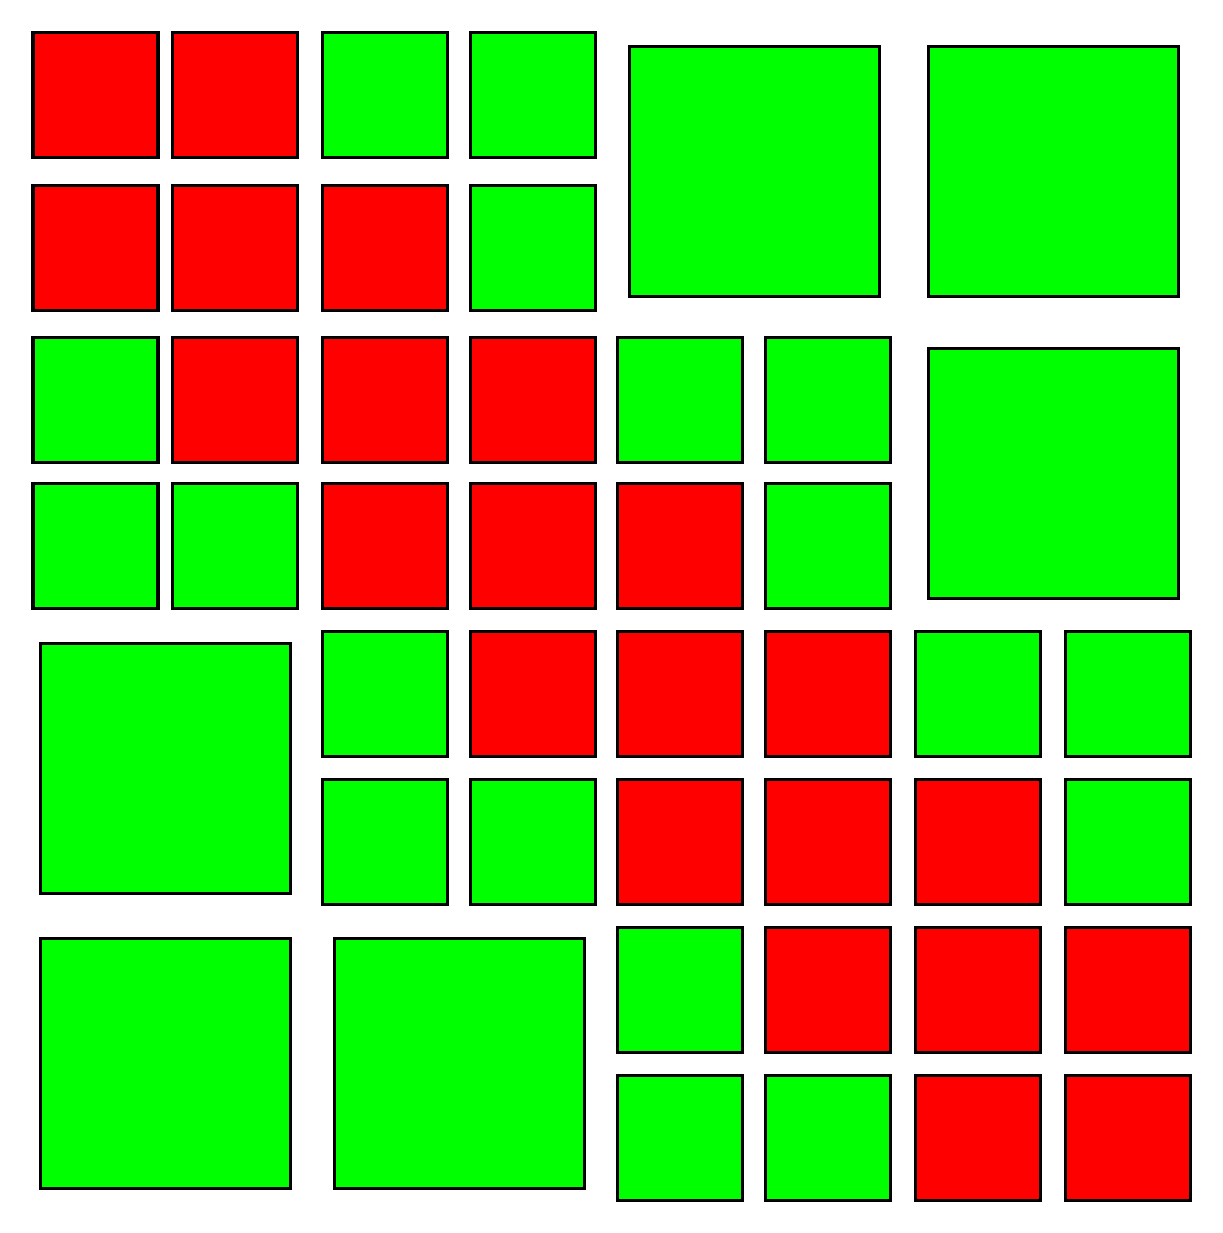
\includegraphics[width=.66\linewidth]{figures/fg-h2-matrix-block.pdf}
        \caption{Betrachte jede Blockmatrix einzeln}
      \onslide<2>
        \centering
        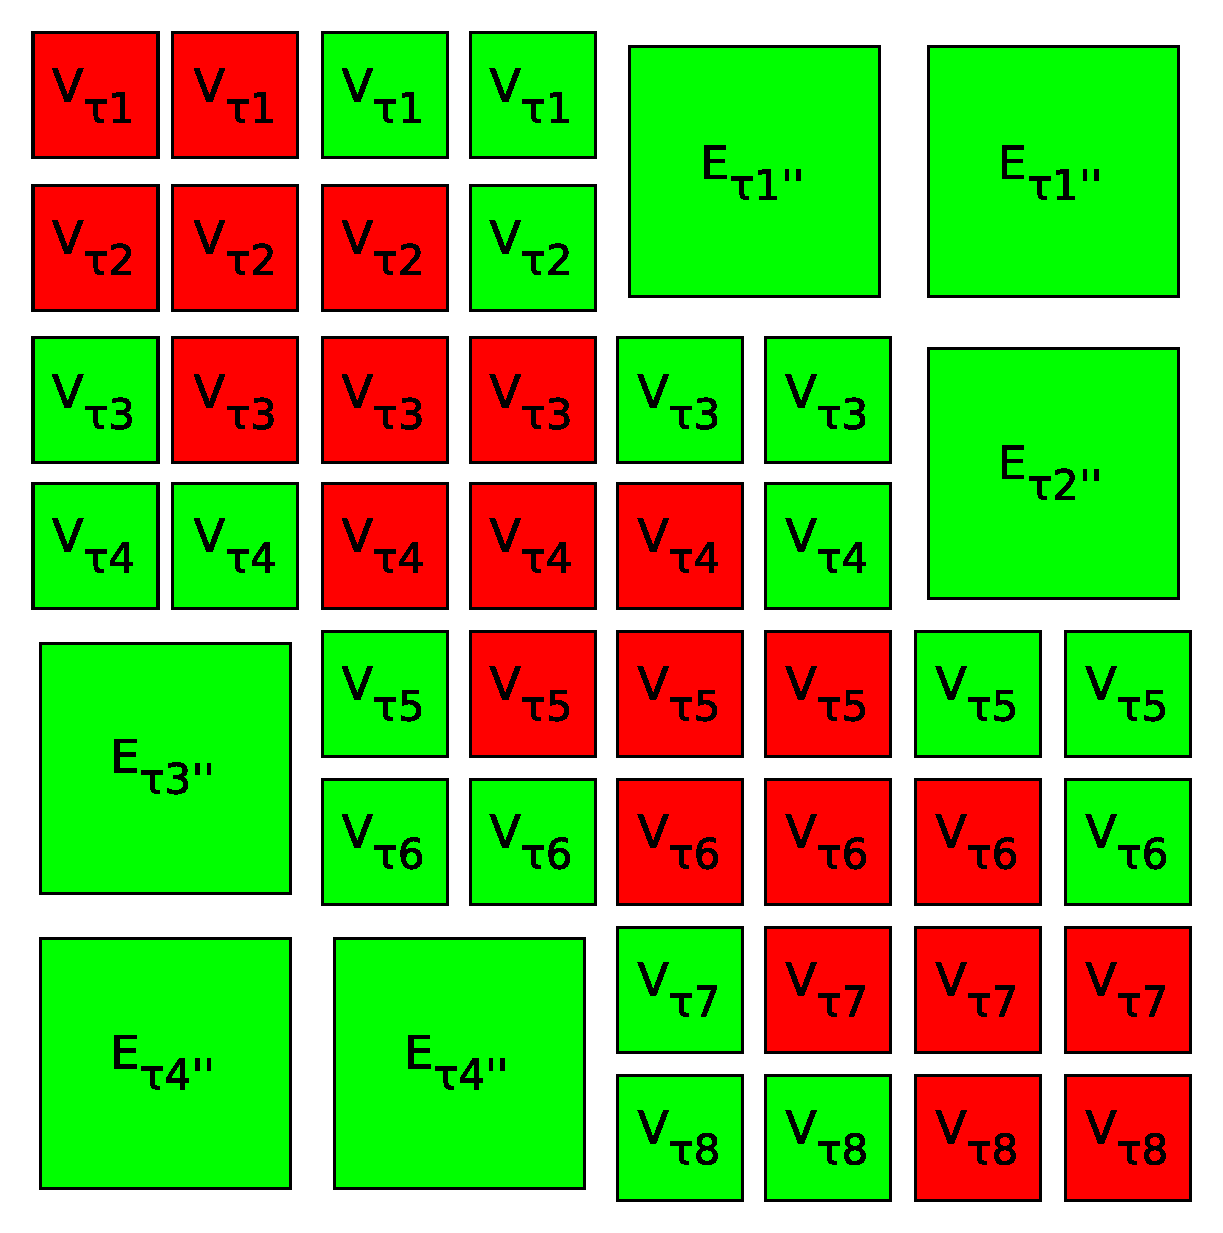
\includegraphics[width=.66\linewidth]{figures/fg-h2-matrix-block-labled.pdf}
        \caption{Kennzeichne die Blockmatrizen mit dem zust\"andigen Zeilencluster}
      \onslide<3>
        \centering
        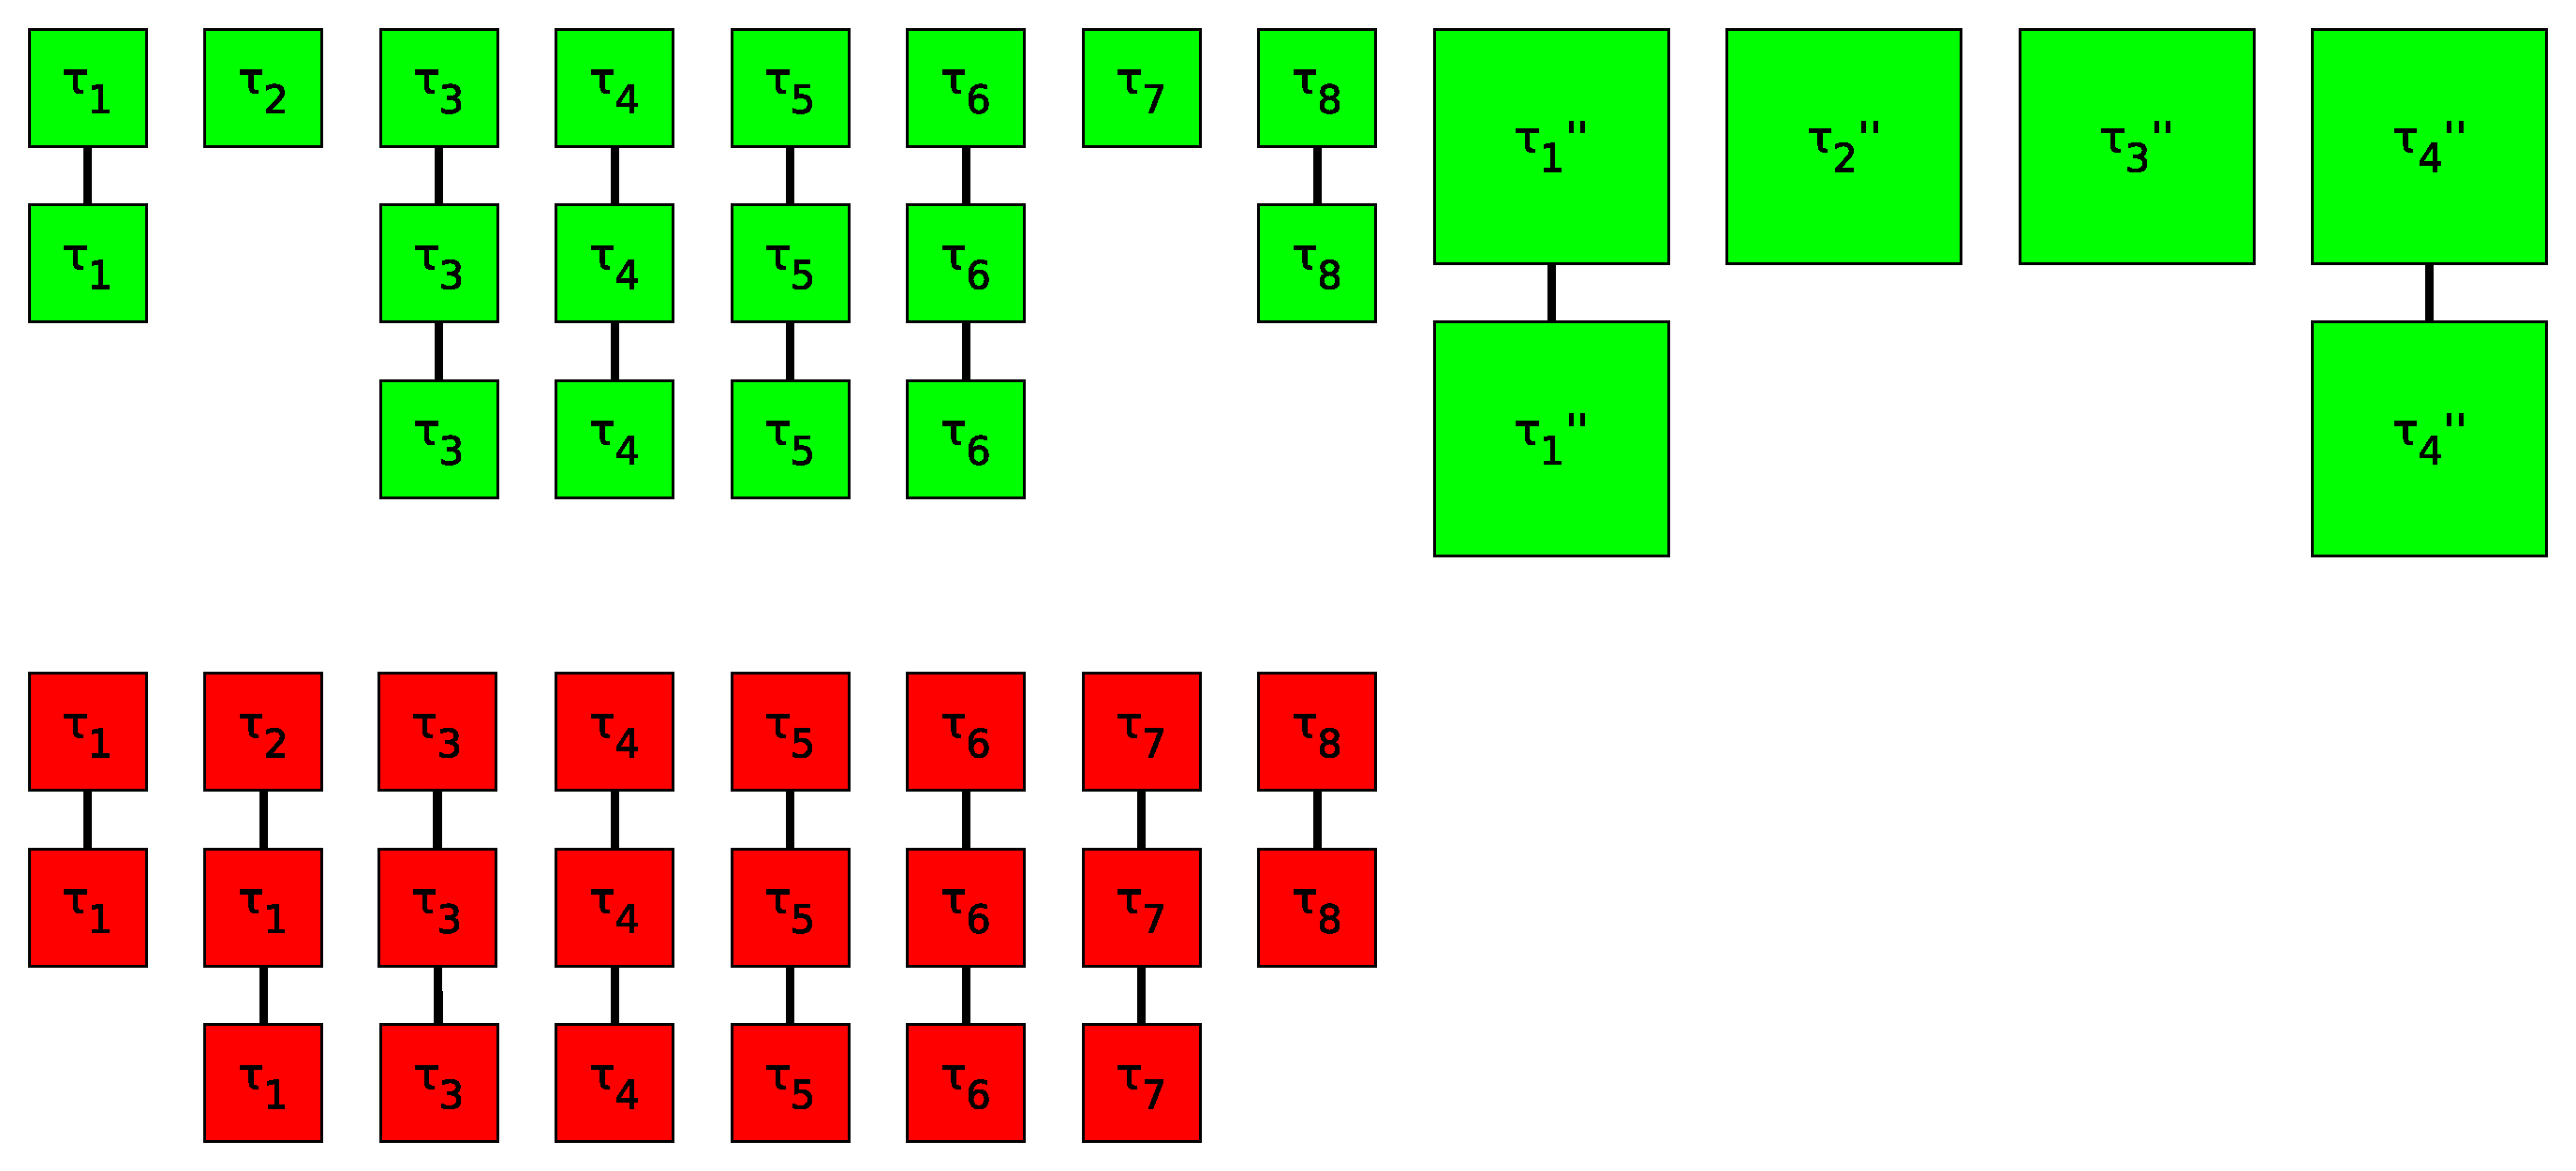
\includegraphics[width=\linewidth]{figures/fg-h2-matrix-block-orderd.pdf}
        \caption{Gruppierung von Blockmatrizen nach Fern- bzw. Nahfeld und nach
                 zust\"andigen Zeilencluster}
    \end{overprint}
  \end{figure}
\end{frame}

\begin{frame}{1. Phase (Fernfeld)}
  \begin{figure}
    \begin{overprint}
      \onslide<1>
        \centering
        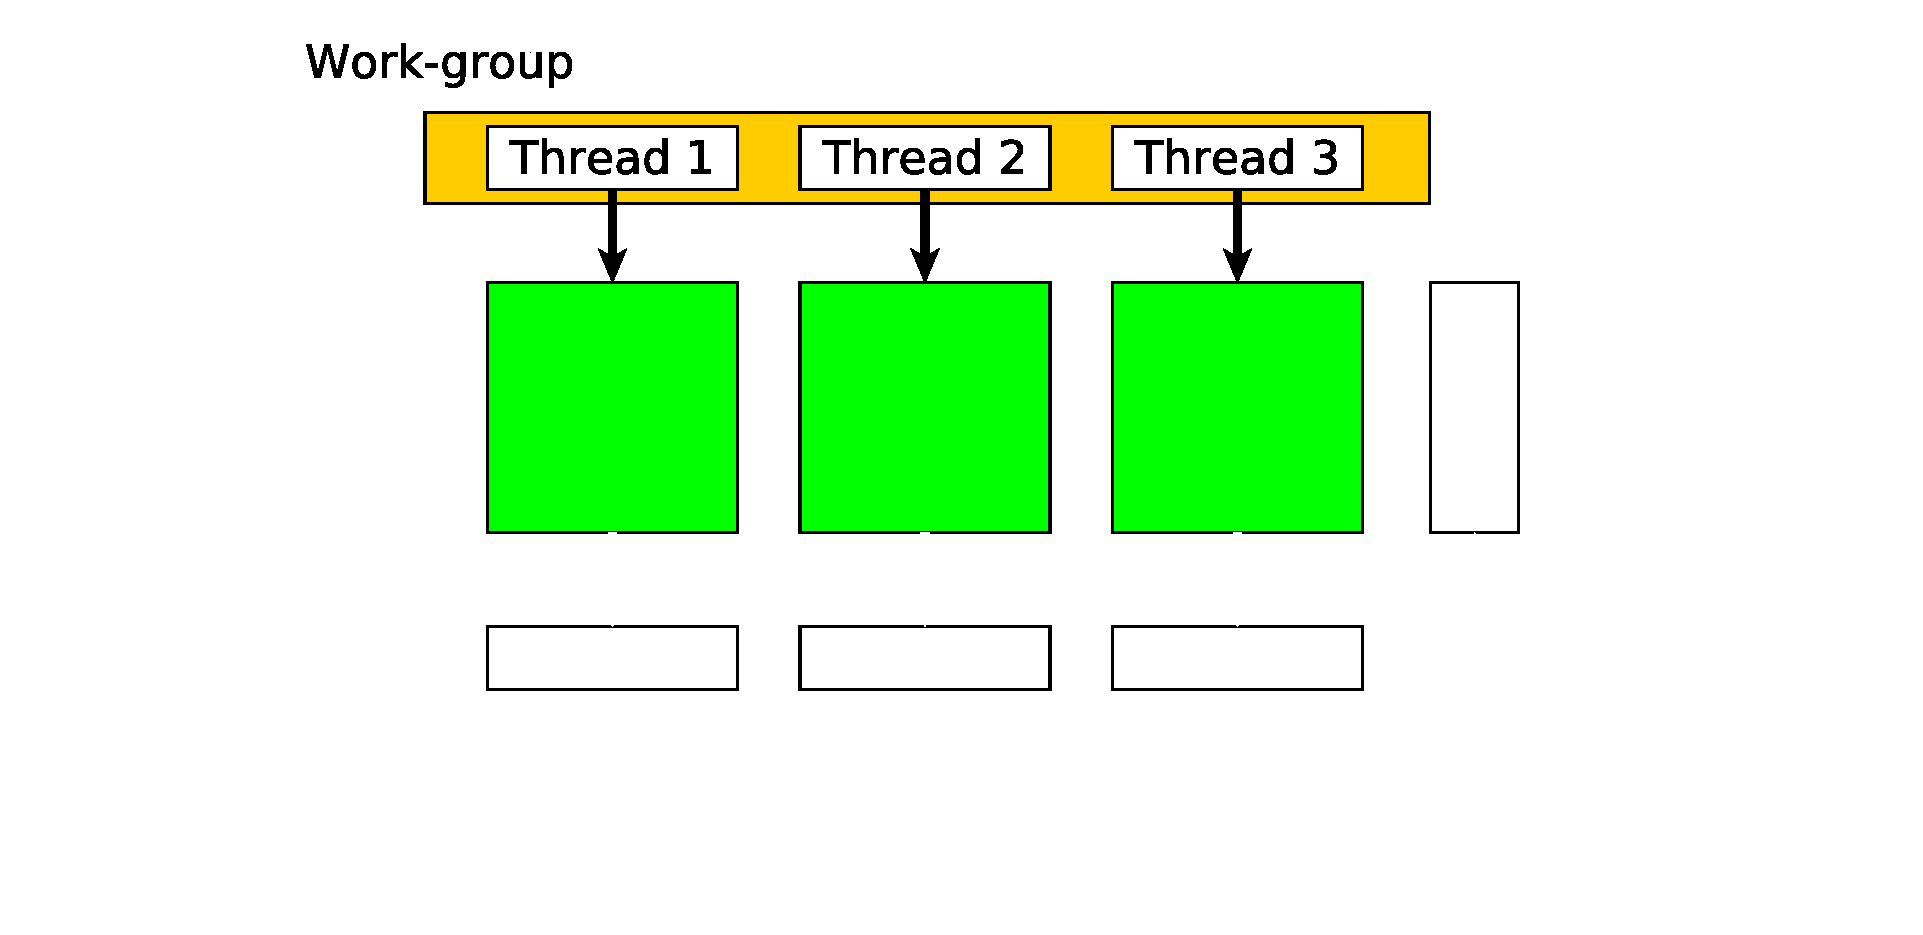
\includegraphics[width=\linewidth]{figures/fg-ff-initial-situation.pdf}
        \caption{Ausgangssituation einer OpenCL work-group in der 1. Phase.}
      \onslide<2>
        \centering
        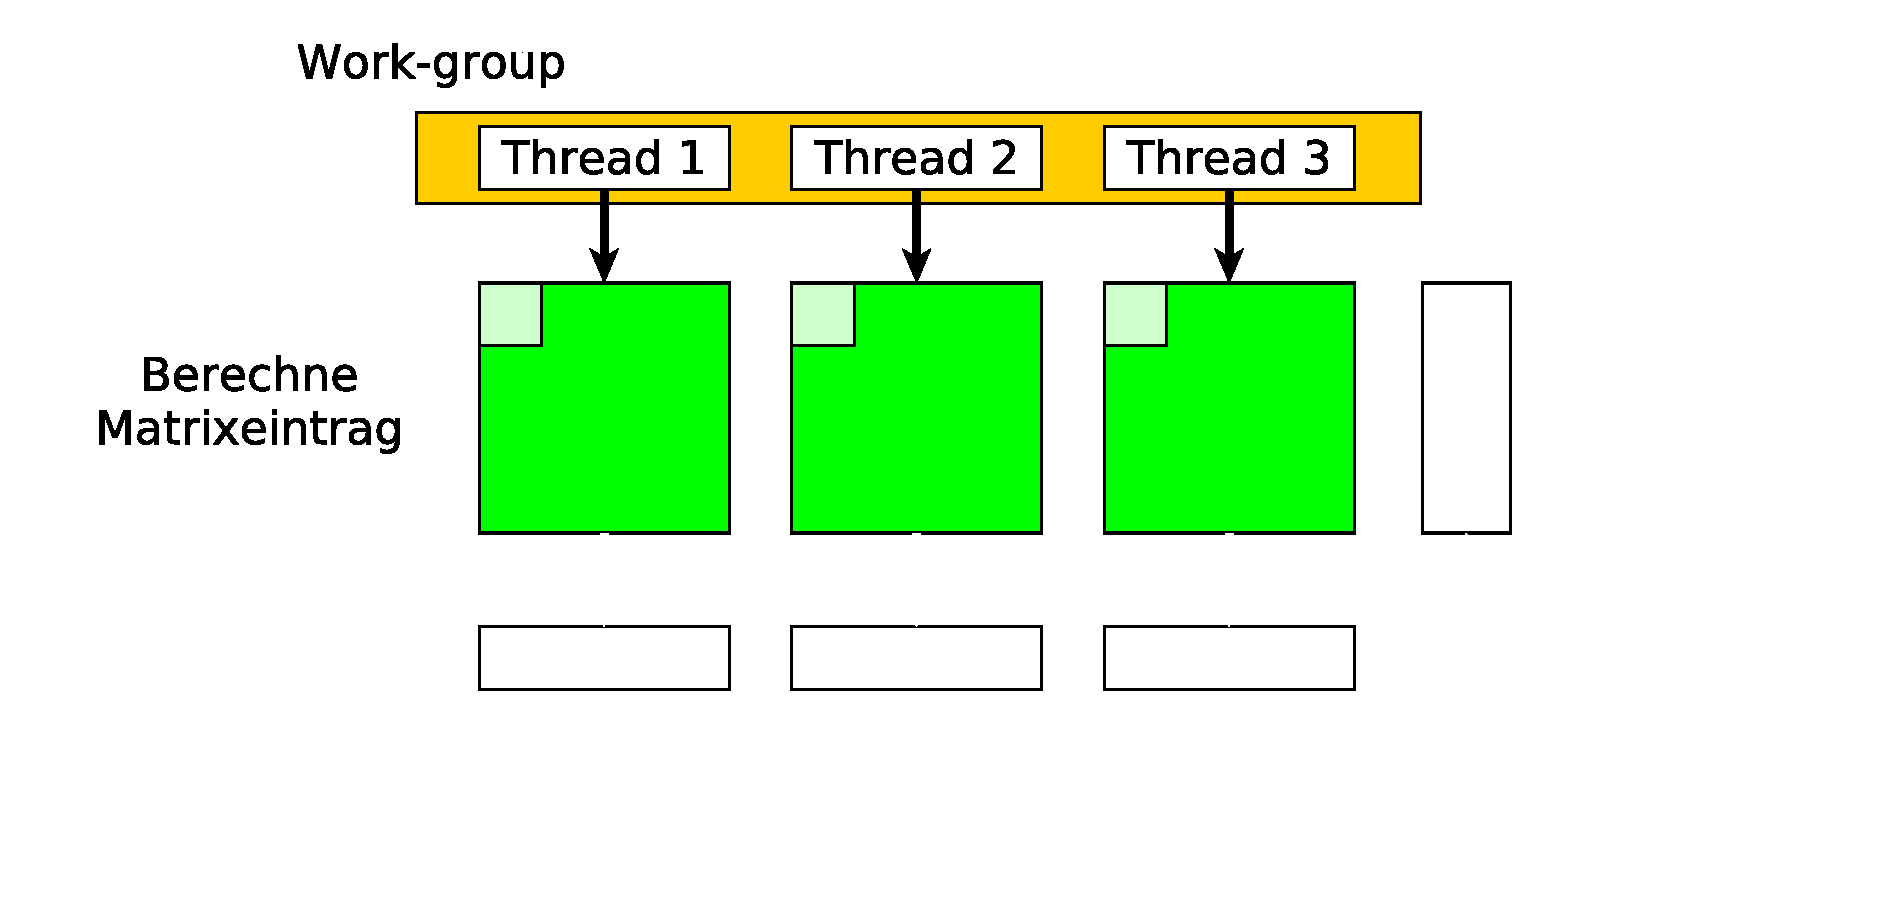
\includegraphics[width=\linewidth]{figures/fg-ff-compute-matrix-entry.pdf}
        \caption{Berechne den ersten Eintrag einer Matrixzeile.}
      \onslide<3>
        \centering
        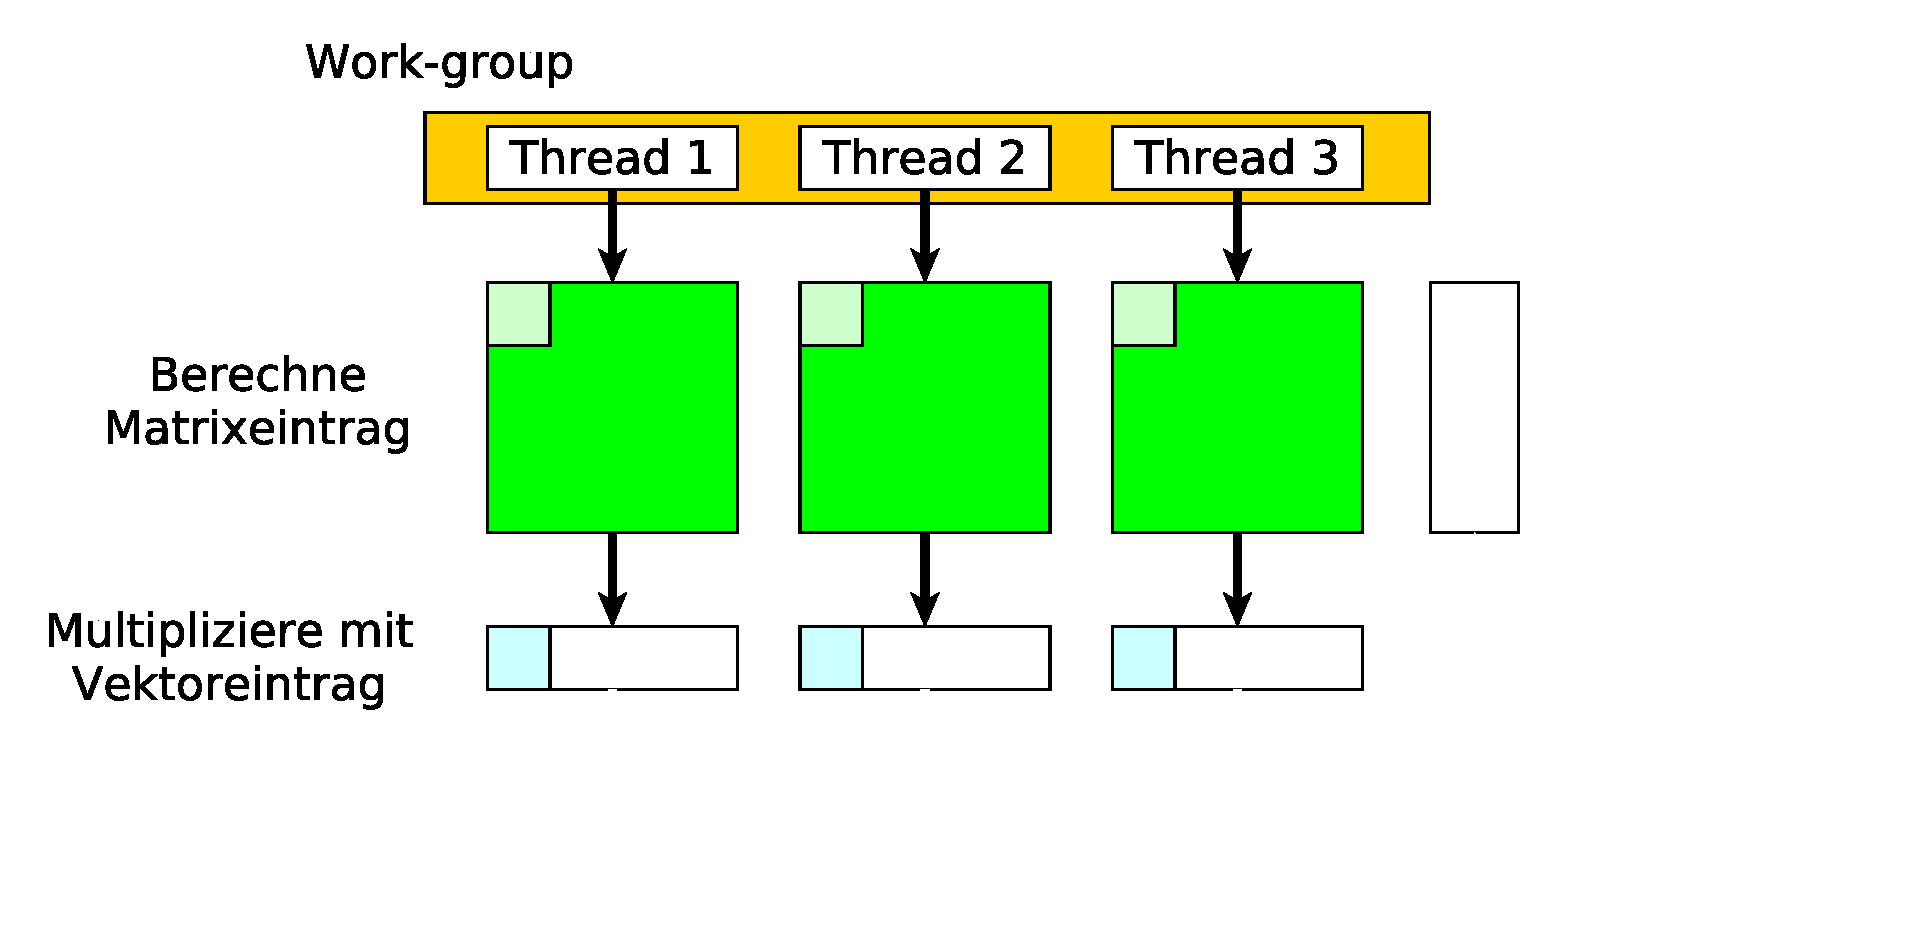
\includegraphics[width=\linewidth]{figures/fg-ff-multiply-vector.pdf}
        \caption{Multipliziere den Matrixeintrag mit dem entsprechenden Eintrag
                 des Eingabevektors.}
      \onslide<4>
        \centering
        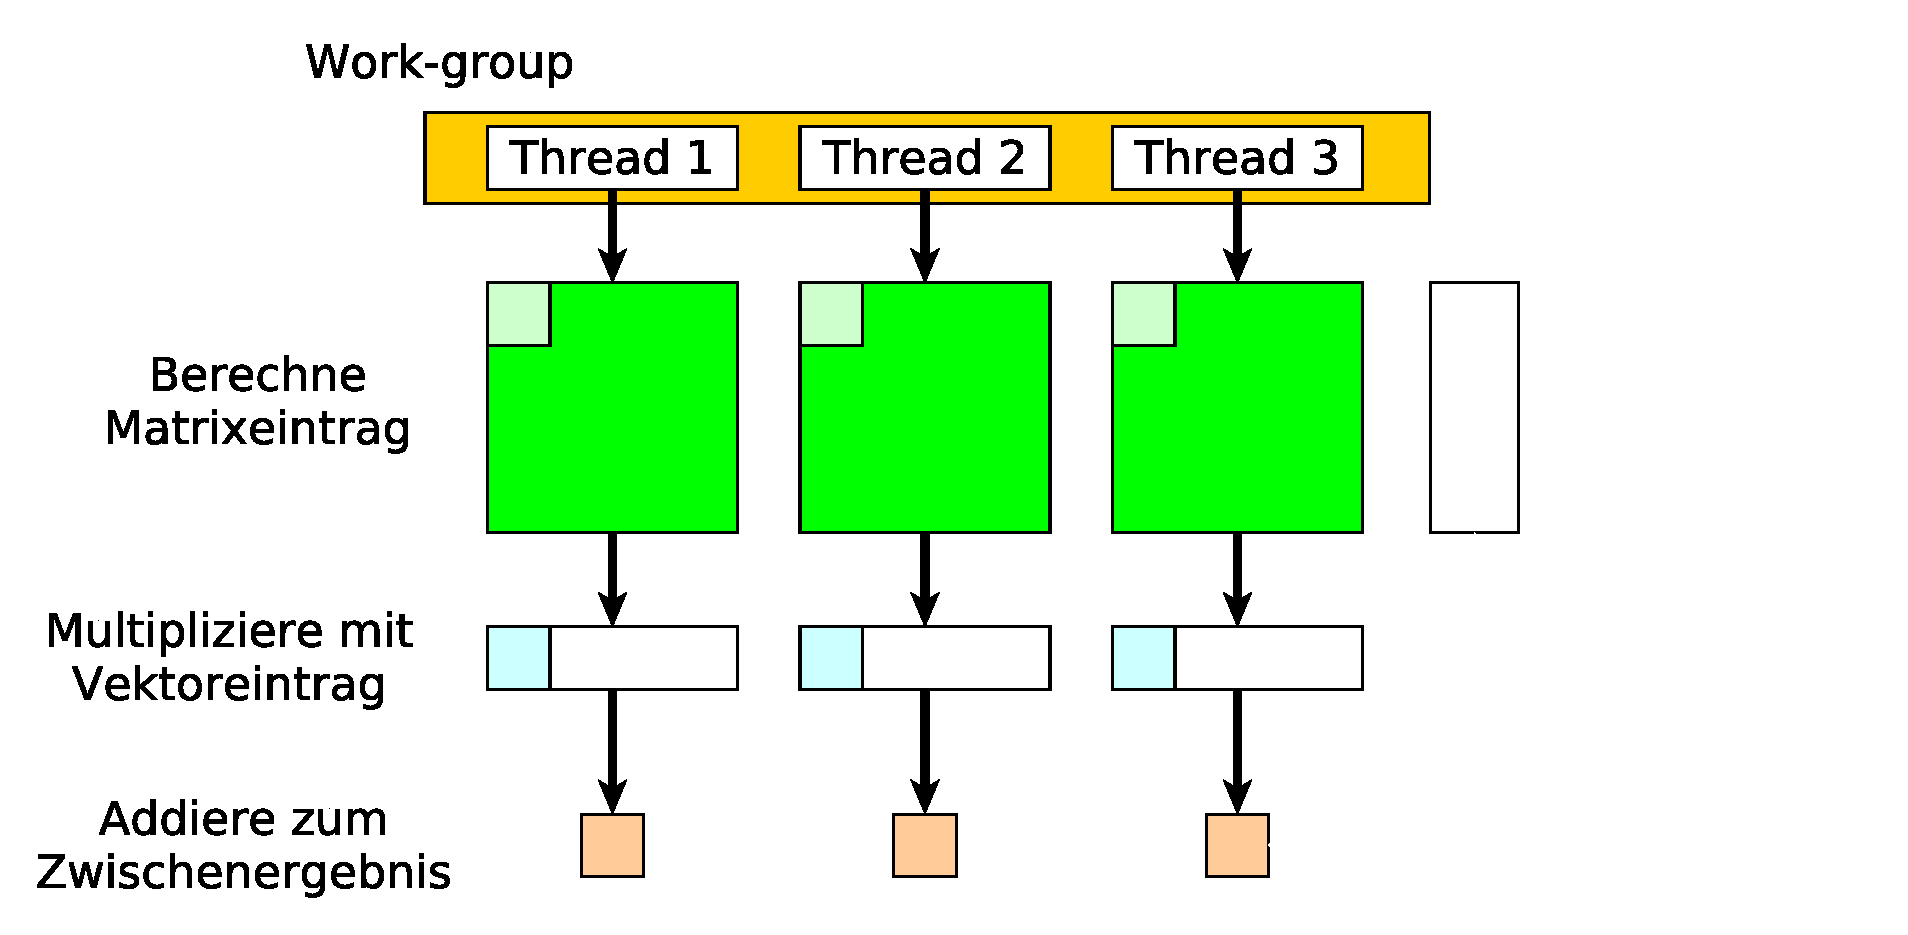
\includegraphics[width=\linewidth]{figures/fg-ff-add-interim-result.pdf}
        \caption{Addiere das Produkt zum Zwischenergebnis hinzu.}
      \onslide<5>
        \centering
        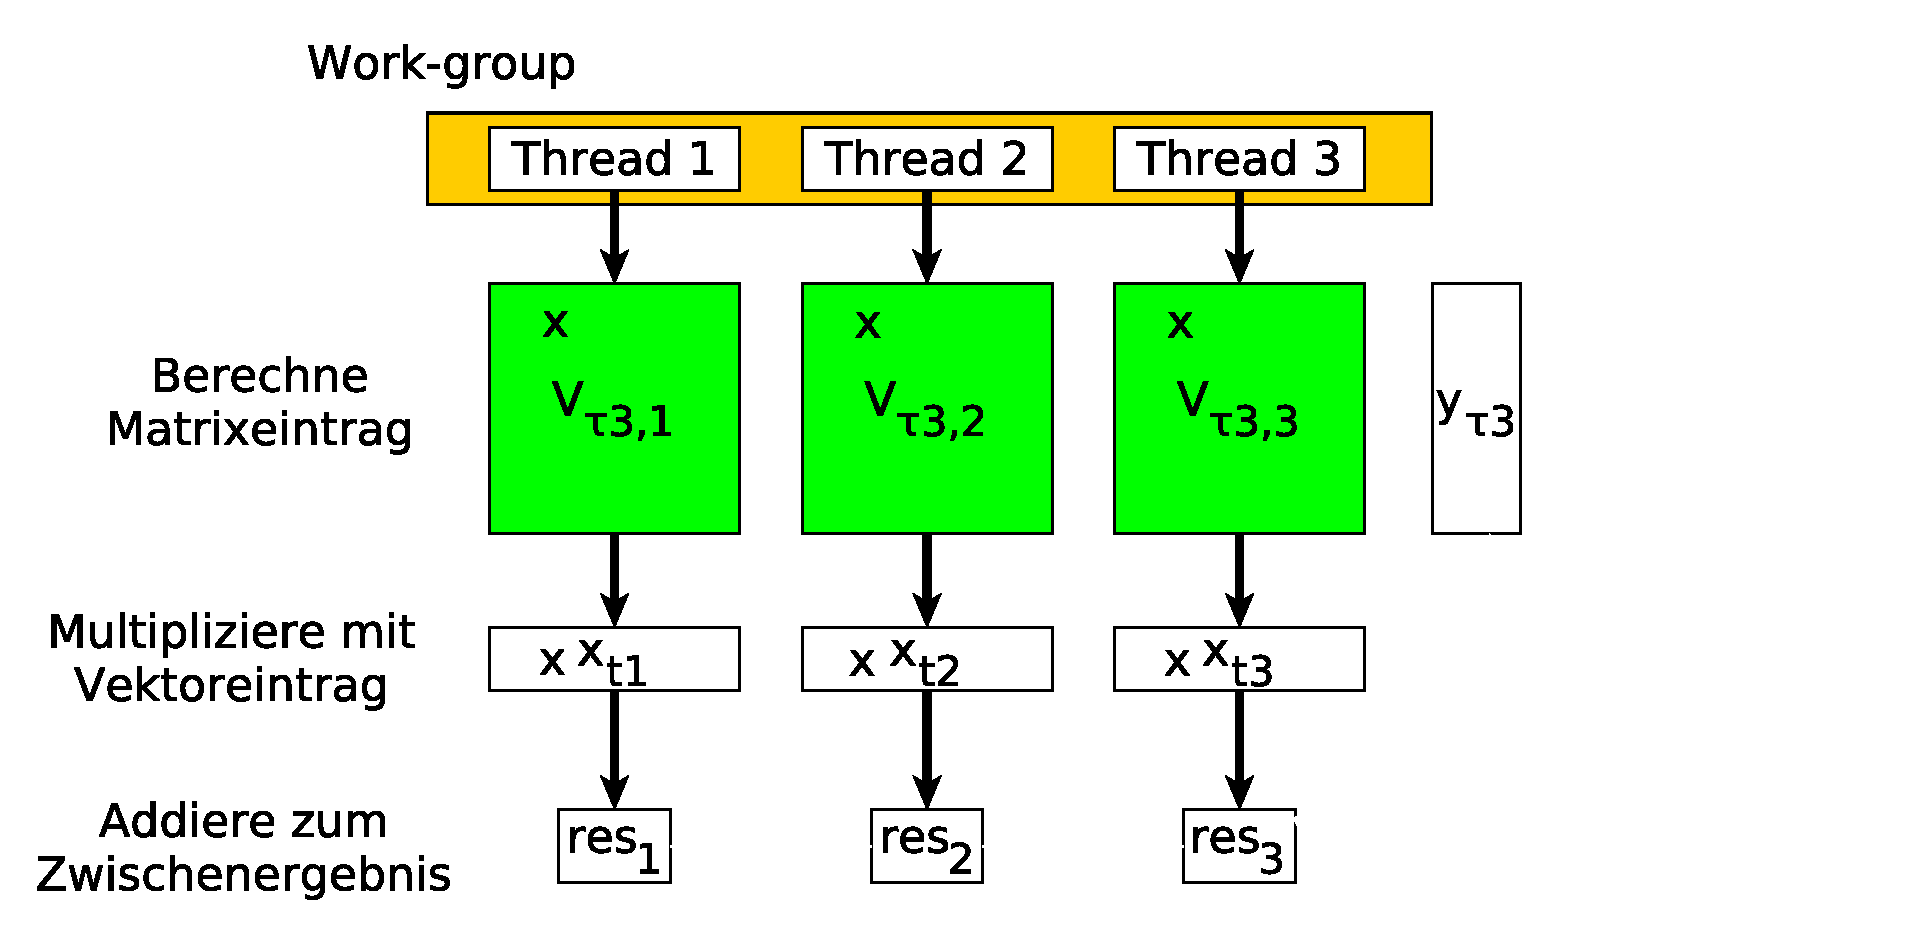
\includegraphics[width=\linewidth]{figures/fg-ff-next-column.pdf}
        \caption{Wiederhole die Prozedur f\"ur alle Eintr\"age einer Zeile.}
      \onslide<6>
        \centering
        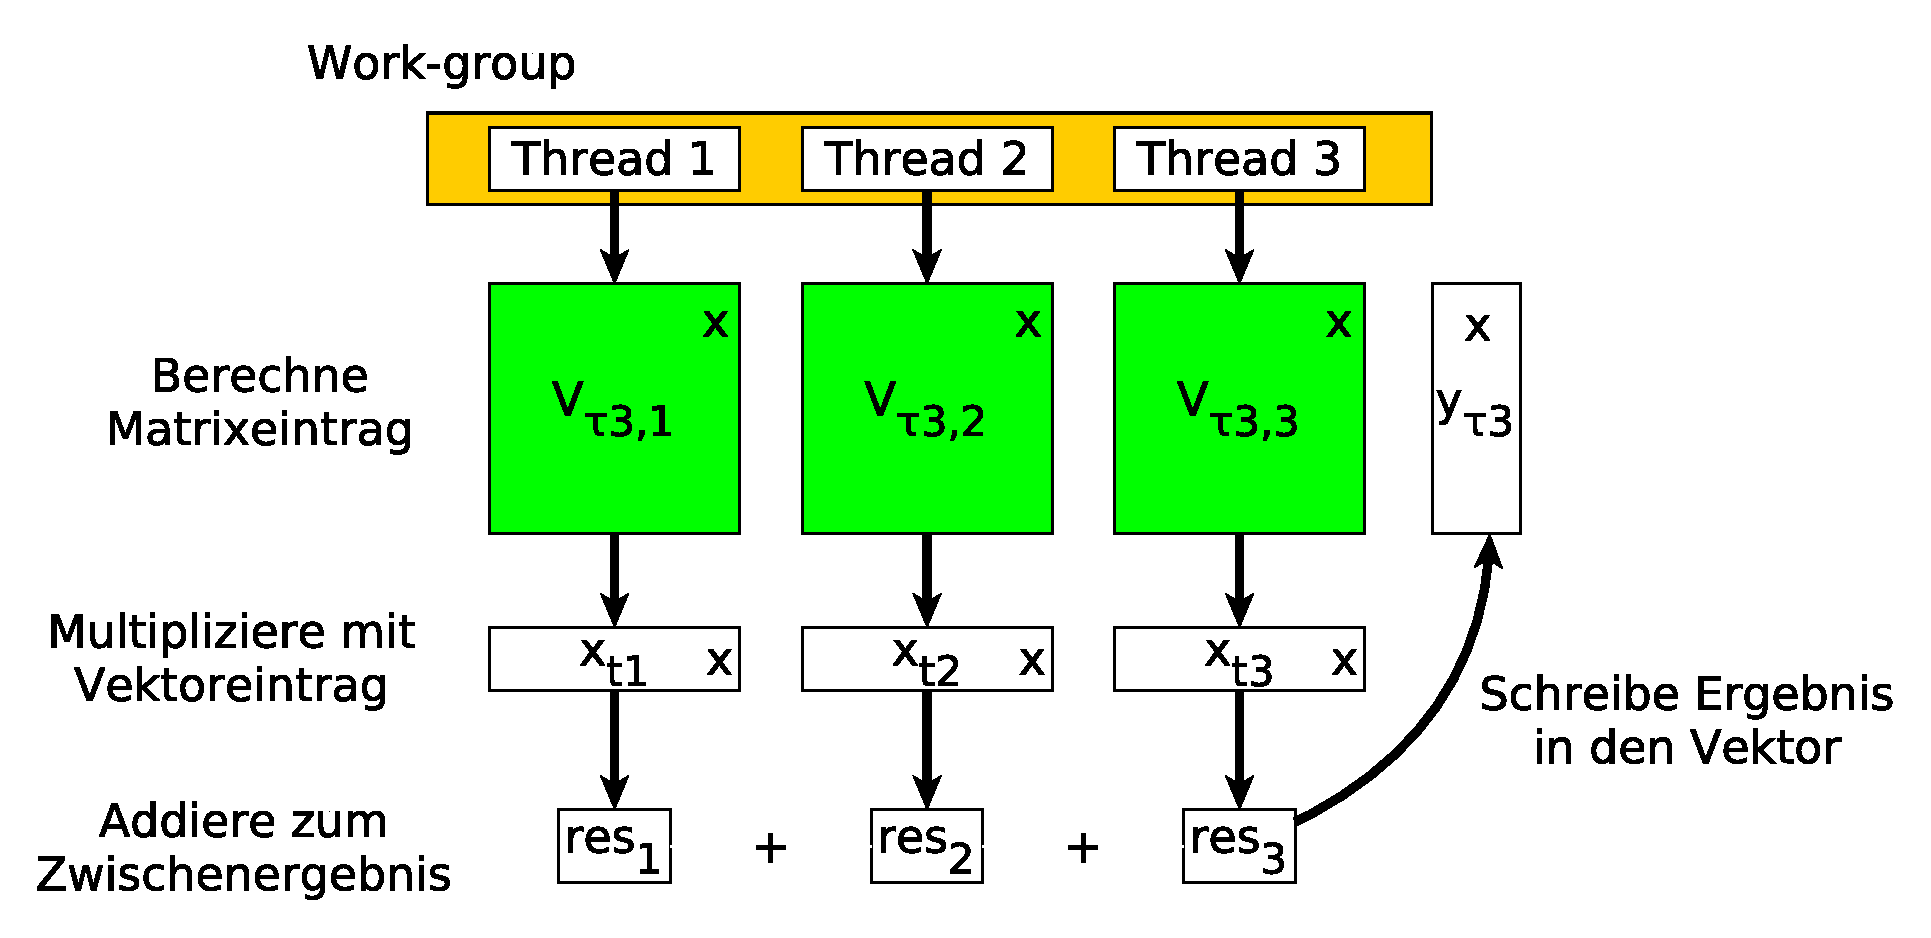
\includegraphics[width=\linewidth]{figures/fg-ff-write-result.pdf}
        \caption{Die Summe der Zwischenergebnisse ergiebt den Eintrag im
                 Ausgabevektor.}
    \end{overprint}
  \end{figure}
\end{frame}

\begin{frame}{1. Phase (Fernfeld)}
  \begin{figure}
    \centering
    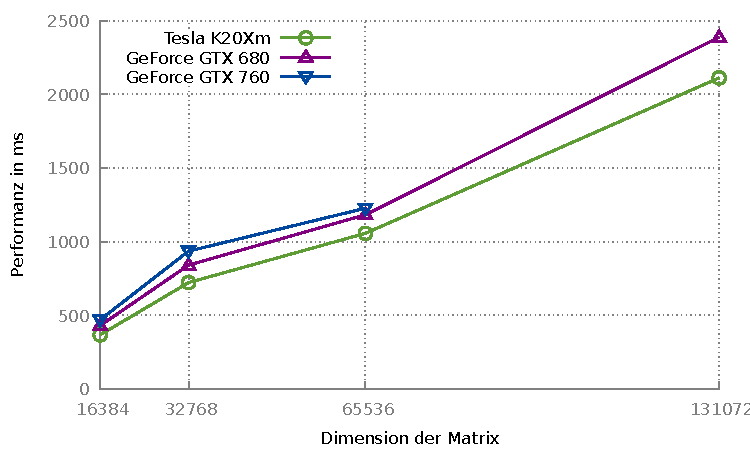
\includegraphics[width=\linewidth]{figures/fg-performance-ff.pdf}
    \caption{Rechenzeit der 1.Phase auf verschiedenen GPUs.}
  \end{figure}
\end{frame}

\begin{frame}{1. Phase (Fernfeld)}
  \small
  \begin{table}
    \begin{tabular}{rrrrrr} \toprule
      \multirow{3}{*}{Dimension} & \multicolumn{5}{c}{Rechenzeit in ms} \\ \cmidrule{2-6}
      & \multicolumn{2}{c}{CPUs} & \multicolumn{3}{c}{GPUs} \\ \cmidrule{2-6}
      & \begin{tabular}{@{}c@{}}Xeon \\ E5-4640\end{tabular}
      & \begin{tabular}{@{}c@{}}Core \\ i7-3820\end{tabular}
      & \begin{tabular}{@{}c@{}}Tesla \\ K20Xm\end{tabular}
      & \begin{tabular}{@{}c@{}}GeForce \\ GTX 680\end{tabular}
      & \begin{tabular}{@{}c@{}}GeForce \\ GTX 760\end{tabular} \\ \cmidrule{1-6}
       16\,384 &  16\,830.000 &  76\,423.179 &  367.612 &  430.675 &  469.848 \\
       32\,768 &  36\,960.000 & 167\,487.521 &  721.806 &  840.885 &  935.754 \\
       65\,536 &  74\,710.000 & 337\,433.000 & 1\,056.583 & 1\,182.343 & 1\,226.704 \\
      131\,072 & 154\,540.000 & 700\,738.240 & 2\,110.852 & 2\,387.168 & --- \\
      \bottomrule
    \end{tabular}
  \end{table}
  \normalsize
\end{frame}

\begin{frame}{2.-3. Phase (Nahfeld)}
  \begin{itemize}
    \item Nahfeld besteht aus allen Integraltypen
    \item Interpertation als Integrale mit unterschiedlichen/unterschiedlich
          vielen Quadraturpunkten
    \item Vertices zweier Dreiecke müssen zueinander permutiert werden
  \end{itemize}
  
  \footnotesize
  \let\thefootnote\relax\footnote{S. A. Sauter und C. Lage.
  \href{https://link.springer.com/article/10.1007\%2Fs00211-015-0757-y}{
  ``On the efficient computation of singular and nearly singular surface 
  integrals arising in 3D-Galerkin BEM''}. In:   \textit{Zeitschrift f\"ur 
  angewandte Mathematik und Mechanik } 76 (1996), S. 273-275.}
  \addtocounter{footnote}{-1}\let\thefootnote\svthefootnote\relax
  \normalsize
\end{frame}

\begin{frame}{2.-3. Phase (Nahfeld)}
  \begin{tabular}{cccccc} \cmidrule[\heavyrulewidth]{1-5}
     & \multicolumn{4}{c}{Anzahl gemeinsamer Vertices} & \\ \cmidrule{2-5}
    \multirow{2}{*}{Anzahl Quadraturpunkte} & 0 & 1 & 2 & 3 & \\ \cmidrule{2-5}
     & k & l & m & m & \(\Leftarrow\) 2.-3. Phase\\
    \cmidrule[\heavyrulewidth]{1-5}
  \end{tabular}
  \begin{itemize}
    \item \(k, l, m \in \mathbb{N}, k < l < m\)
  \end{itemize}

  \footnotesize
  \let\thefootnote\relax\footnote{Steffen Börm u. a. \textit{H2Lib}.
  \url{http://www.h2lib.org/}.}
  \addtocounter{footnote}{-1}\let\thefootnote\svthefootnote\relax
  \normalsize
\end{frame}

\begin{frame}{2.-3. Phase (Nahfeld)}
  \begin{tabular}{cccccc} \cmidrule[\heavyrulewidth]{1-5}
     & \multicolumn{4}{c}{Anzahl gemeinsamer Vertices} & \\ \cmidrule{2-5}
    \multirow{2}{*}{Anzahl Quadraturpunkte} & 0 & 1 & 2 & 3 & \\ \cmidrule{2-5}
     & k & k     & k         & k         & \(\Leftarrow\) 2. Phase \\
     &   & l - k & m - k     & m - k     & \(\Leftarrow\) 3. Phase \\
    \cmidrule[\heavyrulewidth]{1-5}
  \end{tabular}
  \begin{itemize}
    \item \(k, l, m \in \mathbb{N}, k < l < m\)
  \end{itemize}

  \footnotesize
  \let\thefootnote\relax\footnote{Steffen Börm u. a. \textit{H2Lib}.
  \url{http://www.h2lib.org/}.}
  \addtocounter{footnote}{-1}\let\thefootnote\svthefootnote\relax
  \normalsize
\end{frame}

\begin{frame}{2. Phase}
  \begin{itemize}
    \item \"Ahnlich wie in der 1. Phase, bis auf dass
    \begin{itemize}
      \item f\"ur jeden Matrixeintrag entschieden werden muss, welche
            Quadraturpunkte zu wählen sind.
      \item f\"ur jeden Matrixeintrag die entsprechenden Dreiecksvertices
            zueinander permutiert werden müssen.
    \end{itemize}
  \end{itemize}
\end{frame}

\begin{frame}{2. Phase}
  \small
  \begin{table}
    \begin{tabular}{rrrrrr} \toprule
      \multirow{3}{*}{Dimension} & \multicolumn{5}{c}{Rechenzeit in ms} \\ \cmidrule{2-6}
      & \multicolumn{2}{c}{CPUs} & \multicolumn{3}{c}{GPUs} \\ \cmidrule{2-6}
      & \begin{tabular}{@{}c@{}}Xeon \\ E5-4640\end{tabular}
      & \begin{tabular}{@{}c@{}}Core \\ i7-3820\end{tabular}
      & \begin{tabular}{@{}c@{}}Tesla \\ K20Xm\end{tabular}
      & \begin{tabular}{@{}c@{}}GeForce \\ GTX 680\end{tabular}
      & \begin{tabular}{@{}c@{}}GeForce \\ GTX 760\end{tabular} \\ \cmidrule{1-6}
       16\,384 &    900.000 &  4\,547.475 &  72.462 &  64.436 &  75.006 \\
       32\,768 & 1\,780.000 &  9\,167.462 & 138.161 & 125.223 & 147.785 \\
       65\,536 & 3\,550.000 & 18\,162.474 & 273.268 & 246.615 & 291.429\\
      131\,072 & 7\,070.000 & 36\,480.016 & 528.493 & 480.287 & --- \\
      \bottomrule
    \end{tabular}
  \end{table}
  \normalsize
\end{frame}

\begin{frame}{3. Phase}
  \begin{columns}
    \column{0.425\linewidth}
      \begin{algorithm}[H]
        \small{
          \( sum \gets 0 \) \;
          \For{\( q = 0 \to (nq - 1) \)}
          {
            \( sum \gets sum + w_{q} * kernel\relax(x_{q}, \ y_{q}) \) \;
          }
          \( result \gets result + sum \) \;
        }
      \end{algorithm}
    \column{0.6\linewidth}
      \begin{algorithm}[H]
        \small{
        \( lid \gets \) get\_local\_id\relax(0) \;
        \( lsize \gets \) get\_local\_size\relax(0) \;
        \( sum_{lid} \gets 0 \) \;
        \( q \gets 0 \) \;
        \While{\( q < nq \)}
        {
          \If{\( (q + lid) < nq \)}
          {
            \( sum_{lid} \gets sum_{lid} + w_{q + lid} *
               kernel\relax(x_{q + lid}, y_{q + lid}) \) \;
          }

          \( nq \gets nq + lsize \) \;
        }

        \( result \gets results + \sum\limits_{i = 0}^{lsize - 1} sum_{i} \) \;
        }
      \end{algorithm}
      % \begin{algorithm}[H]
      %   \begin{algorithmic}[1]
      %     \footnotesize
      %     {
      %     \State{lid = get\_local\_id\relax(0)}
      %     \State{lsize = get\_local\_size\relax(0)}
      %     \State{sum = 0}
      %     \For{q = 0; q < nq; q += lsize}
      %       \If{(q + lid) < nq}
      %         \State{\(sum_{lid}\) += \(w_{q + lid}\) * kernel\relax(\(x_{q + lid}, y_{q + lid}\))}
      %       \EndIf{}
      %     \EndFor{}
      %     }
      %     \State{result += \(\sum\limits_{i = 0}^{lsize} sum_{i}\)}
      %   \end{algorithmic}
      % \end{algorithm}
  \end{columns}
  \begin{center}
    Pseudocode zum sequentiellen (links) und Thread-level vektorisierten
    (rechts) Auswerten einer Quadratur.
  \end{center}
\end{frame}

\begin{frame}{3. Phase}
  \small
  \begin{table}[ht]\label{tab:fevalnfu}
    \begin{tabular}{rrrrrr} \toprule
      \multirow{3}{*}{Dimension} & \multicolumn{5}{c}{Rechenzeit in ms} \\
      \cmidrule{2-6}
      & \multicolumn{2}{c}{CPUs} & \multicolumn{3}{c}{GPUs} \\ \cmidrule{2-6}
      & \begin{tabular}{@{}c@{}}Xeon \\ E5-\relax4640\end{tabular}
      & \begin{tabular}{@{}c@{}}Core \\ i7-\relax3820\end{tabular}
      & \begin{tabular}{@{}c@{}}Tesla \\ K20Xm\end{tabular}
      & \begin{tabular}{@{}c@{}}GeForce \\ GTX 680\end{tabular}
      & \begin{tabular}{@{}c@{}}GeForce \\ GTX 760\end{tabular} \\ \cmidrule{1-6}
       16\,384 &    710.000 &  4\,005.020 &  95.714 & 122.481 & 109.927 \\
       32\,768 & 1\,420.000 &  8\,096.907 & 185.583 & 248.359 & 216.954 \\
       65\,536 & 2\,800.000 & 16\,019.292 & 359.989 & 463.968 & 433.221 \\
      131\,072 & 5\,680.000 & 32\,403.679 & 721.983 & 995.758 & --- \\
      \bottomrule
    \end{tabular}
  \end{table}
  \normalsize
\end{frame}


\begin{frame}{1.-3.Phase im Vergleich}
  \begin{figure}
    \centering
    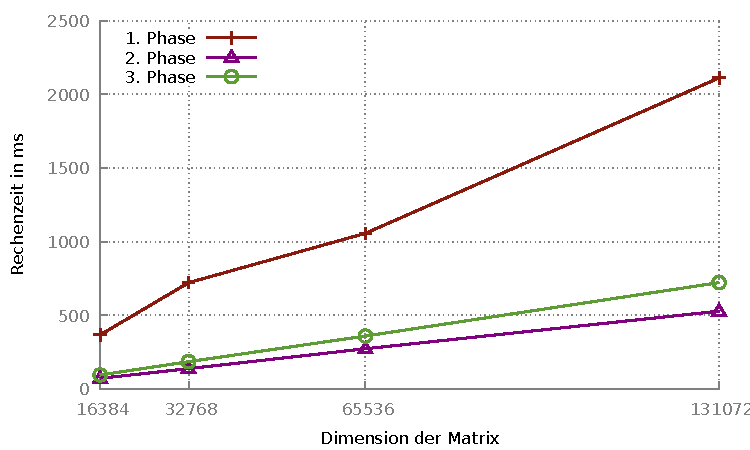
\includegraphics[width=\linewidth]{figures/fg-performance-feval-1-3.pdf}
    \caption{Rechenzeit der einzelnen Phasen im Vergleich auf einer Tesla
             K20xm.}
  \end{figure}
\end{frame}


\begin{frame}{Optimierung: Lokalit\"at von Speicher}
  \begin{algorithm}[H]
    \SetKwProg{Proc}{}{}{}
    \Proc{fastaddeval\_farfield}
    {
      \For{\( i = 0 \to (rows - 1) \)}
      {
        // Hole Informationen \"uber Zeile i \\
        \For{\( j = 0 \to (cols - 1) \)}
        {
          // Hole Informationen \"uber Spalte j \\

          \For{\( q = 0 \to (nq - 1) \)}
          {
            // F\"uhre Quadratur bzgl. i, j und q-ten Quadraturpunkt \\
            // und -gewicht durch.
          }
        }
      }      
    }
    \caption{Verschachtelte Schleifen in der 1. Phase. Eine tiefere
             Verschachtelungsebene bedeutet mehr Speicherzugriffe.}
  \end{algorithm}
\end{frame}

\begin{frame}{Optimierung: Lokalit\"at von Speicher}
  \begin{figure}
    \centering
    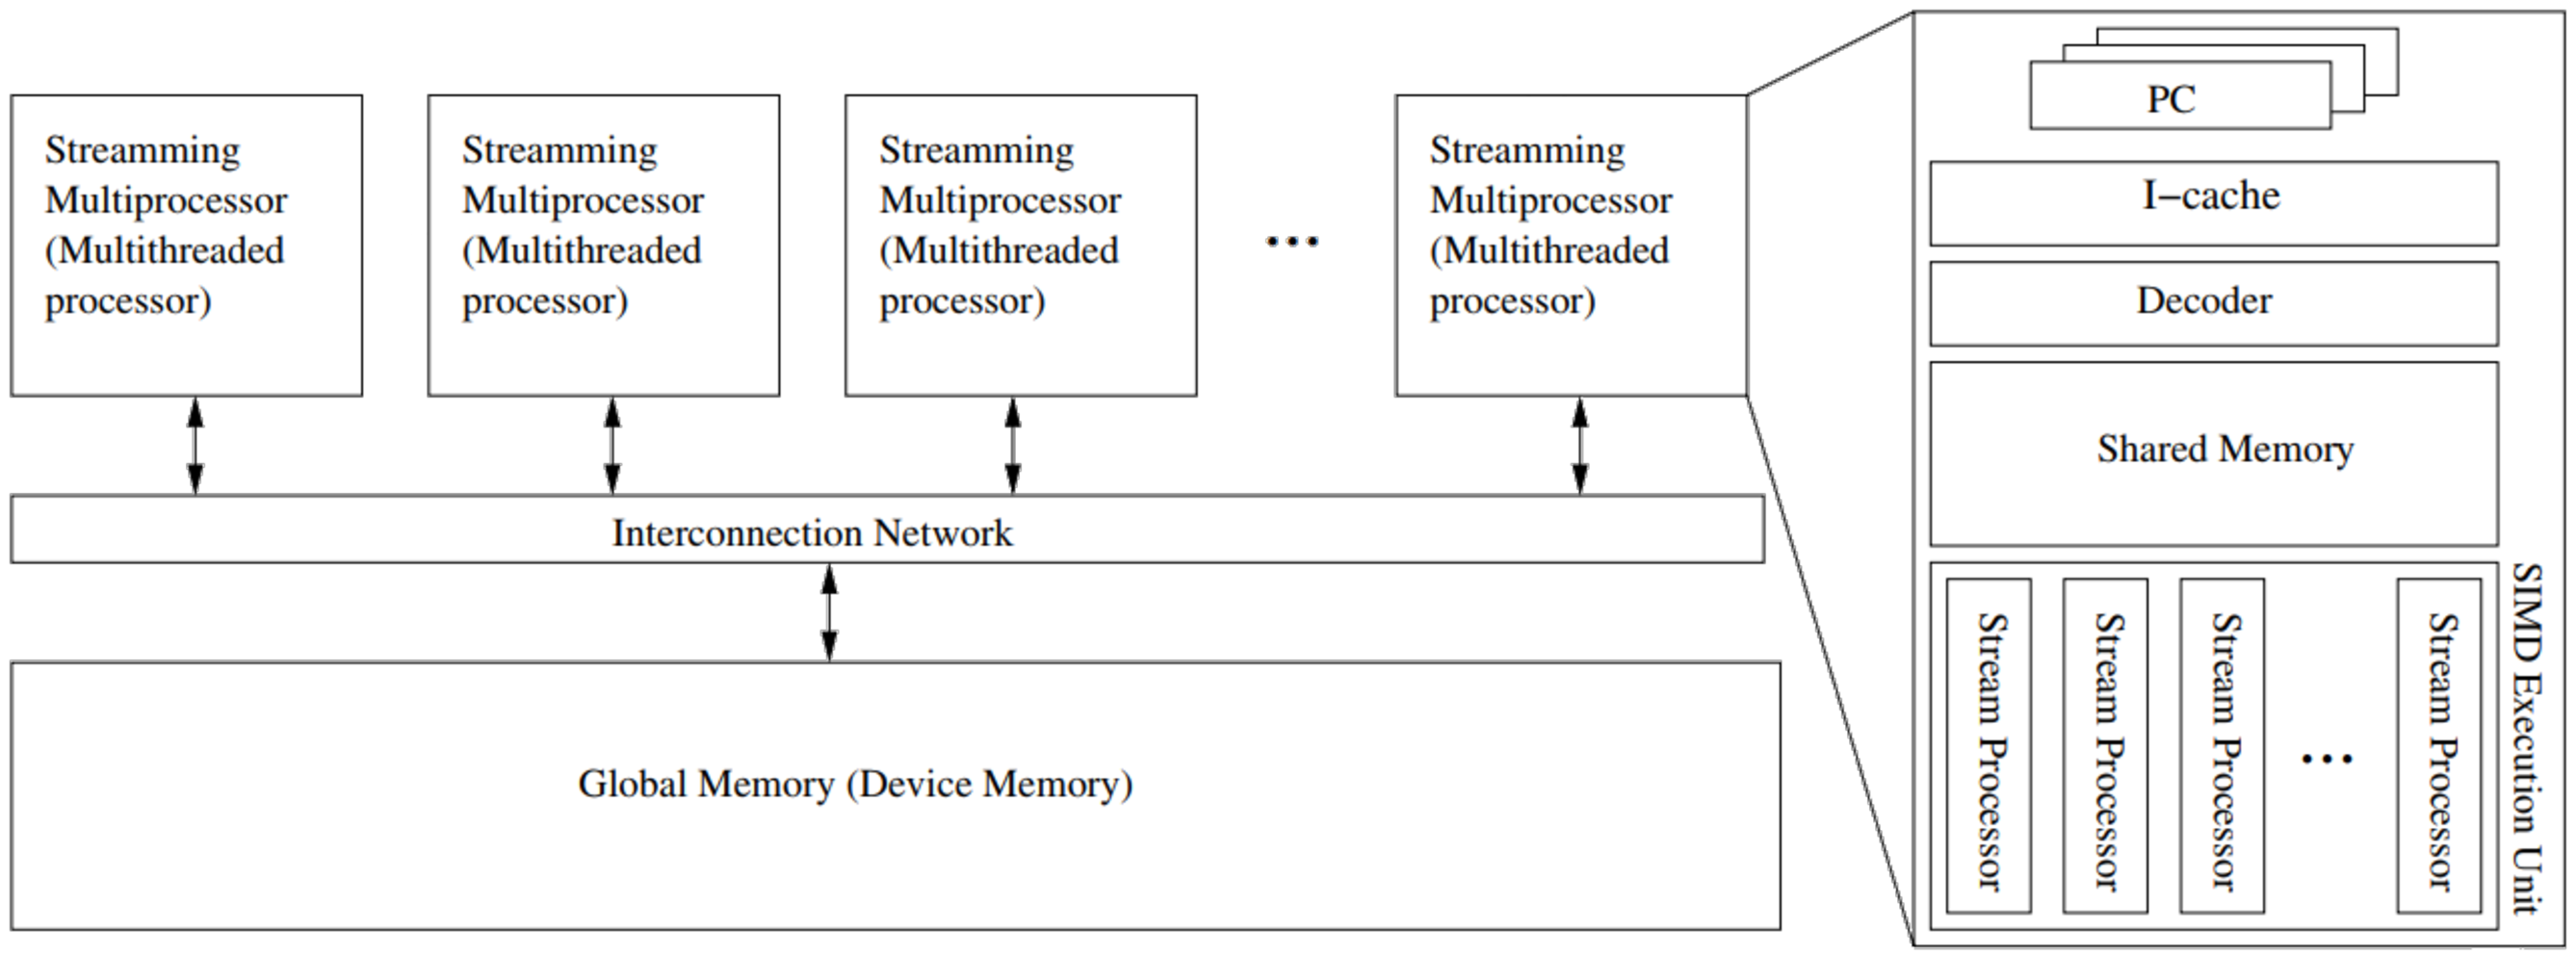
\includegraphics[width=\linewidth]{figures/fg-gpu_architecture.pdf}
    \caption{Erinnerung: (Speicher-)Architektur einer Grafikkarte.}
  \end{figure}
\end{frame}

\begin{frame}{Optimierung: Lokalität von Speicher}
  \small
  \begin{table}
    \begin{tabular}{rrr} \toprule
      \multirow{3}{*}{Dimension} & \multicolumn{2}{c}{Rechenzeit in ms} \\ \cmidrule{2-3}
      & \multicolumn{2}{c}{Lokalität der Quadraturpunkte} \\ \cmidrule{2-3}
      & Globaler Speicher & Lokaler Speicher \\ \cmidrule{1-3}
       16\,384 &    367.612 &    305.763  \\ %324 bytes
       32\,768 &    721.806 &    614.329  \\
       65\,536 & 1\,056.583 &    805.513  \\
      131\,072 & 2\,110.852 & 1\,665.412 \\
      \bottomrule
    \end{tabular}
    \caption{Performanzvergleiche von der Verfügbarkeit von Quadraturpunkten
             in unterschiedlichen Speicherbereichen auf einer Tesla K20Xm.}
  \end{table}
  \normalsize
\end{frame}

\begin{frame}{Optimierung: Vektorisierung auf Instruktionsebene}
  \begin{itemize}
    \item z.B. float2, float4, float8, float16 in OpenCL
    \item Abstrahieren die Vektorregister der unterliegenden Architektur
    \item SSE/AVX auf CPUs (falls vorhanden)
    \item NVIDIAs Skalarprozessoren besizten keine Vektoreinheiten
    \begin{itemize}
      \item Vektorisierte Speicherzugriffe können jedoch zusammengefasst
            werden.
      \item Vektorisierte Rechenoperationen werden durch skalare simuliert
      \item Höhere Anzahl an Register werden benötigt
    \end{itemize}
  \end{itemize}
\end{frame}

\begin{frame}{Optimierung: Vektorisierung auf Instruktionsebene}
  \begin{table}[ht]\label{tab:vec}
    \begin{tabular}{rrr} \toprule
      \multirow{3}{*}{Dimension} & \multicolumn{2}{c}{Rechenzeit in ms} \\ 
      \cmidrule{2-3}
      & \multicolumn{2}{c}{Vektorbreite} \\ \cmidrule{2-3}
      & 1 & 4 \\ \midrule
       16\,384 &    305.763 &    286.222 \\
       32\,768 &    614.329 &    581.817 \\
       65\,536 &    805.513 &    763.979 \\
      131\,072 & 1\,665.412 & 1\,562.938 \\
      \bottomrule
    \end{tabular}
    \caption{Performanzvergleich unterschiedlicher Vektorbreiten, verwendet zur
             vektorisierten Berechnung der Quadratur.}
  \end{table}
\end{frame}

\section{Zusammenfassung \& Ausblick}

\begin{frame}{Zusammenfassung}
  \begin{table}[ht]\label{tab:mvm}
    \resizebox{\textwidth}{!}
    {
      \begin{tabular}{rrrrrrrr} \toprule
        \multirow{4}{*}{Dimension} & \multicolumn{7}{c}{Rechenzeit in ms} \\
        \cmidrule{2-8}
        & \multirow{3}{*}{\( \mathcal{H}^2 \)-MVM}
        & \multicolumn{6}{c}{Ordnung} \\ \cmidrule{3-8}
        & & \multicolumn{2}{c}{2} & \multicolumn{2}{c}{3} & \multicolumn{2}{c}{4}
        \\ \cmidrule{3-8}
        & 
        & \begin{tabular}{@{}c@{}}
            \( \mathcal{H}^2 \)-MVM \\
            (CPU)
          \end{tabular}
        & \begin{tabular}{@{}c@{}}
            \( \mathcal{H}^2 \)-MVM \\
            (GPU)
          \end{tabular}
        & \begin{tabular}{@{}c@{}}
            \( \mathcal{H}^2 \)-MVM \\
            (CPU)
          \end{tabular}
        & \begin{tabular}{@{}c@{}}
            \( \mathcal{H}^2 \)-MVM \\
            (GPU)
          \end{tabular}
        & \begin{tabular}{@{}c@{}}
            \( \mathcal{H}^2 \)-MVM \\
            (CPU)
          \end{tabular}
        & \begin{tabular}{@{}c@{}}
            \( \mathcal{H}^2 \)-MVM \\
            (GPU)
          \end{tabular} \\ \midrule
         16\,384 &    140 &  6\,980 &    500 &  19\,770 &    950 &  50\,730 &
          2\,350 \\
         32\,768 &    300 & 14\,640 & 1\,000 &  43\,600 & 1\,820 & 106\,770 &
          4\,530 \\
         65\,536 &    660 & 29\,440 & 1\,490 &  94\,740 & 2\,940 & 220\,670 &
          8\,280 \\
        131\,072 & 1\,190 & 60\,920 & 3\,030 & 194\,980 & 5\,840 & 452\,060 & 
         16\,320 \\
        \bottomrule
      \end{tabular}
    }
  \end{table}
  \begin{itemize}
    \item Wir können den Speicherbedarf einer \(\mathcal{H}^2\)-Matrix um
          75 bis 90\% reduzieren
    \item Die benötigte Rechenzeit kann auf GPUs um einen Faktor 20 bis 50
          reduziert werden verglichen mit einer CPU-Implementierung
    \item Rechenaufwand jedoch höher als bei einer reinen
          Matrix-Vektor-Multiplikation (und nimmt zusätzlich mit höherer
          Quadraturordnung zu)
  \end{itemize}
\end{frame}

\begin{frame}{Zusammenfassung}
  \small
  \begin{table}
    \begin{tabular}{rrr} \toprule
                & \multicolumn{2}{c}{Performanz in ms} \\ \cmidrule{2-3}
      Dimension & \(\mathcal{H}^2\)-Matrix & Blockmatrizen \\ \midrule
          16\,384 &                     131\,620 &   63\,310 \\
          32\,768 &                     267\,940 &  109\,092 \\
          65\,536 &                     530\,570 &  271\,120 \\
         131\,072 &                  1\,073\,480 &  559\,450 \\ \bottomrule
      \end{tabular}
    \end{table}
  \normalsize
  \begin{itemize}
    \item Setup-Zeit lässt sich um die Hälfte reduzieren
  \end{itemize}
\end{frame}

\begin{frame}{Ausblick}
  \begin{itemize}
    \item Parallelisierung des hostseitigen Codes?
    \item Multi-GPU\@?
    \item Auslagern der Vorwärts- und Rückwärtstransformation auf GPUs?
  \end{itemize}
\end{frame}
\begin{frame}[allowframebreaks]{Literatur}

  \printbibliography
  \nocite{*}

\end{frame}

\begin{frame}
  \Huge Vielen Dank! Fragen?
\end{frame}
\end{document}
